\documentclass[twoside]{book}

% Packages required by doxygen
\usepackage{fixltx2e}
\usepackage{calc}
\usepackage{doxygen}
\usepackage[export]{adjustbox} % also loads graphicx
\usepackage{graphicx}
\usepackage[utf8]{inputenc}
\usepackage{makeidx}
\usepackage{multicol}
\usepackage{multirow}
\PassOptionsToPackage{warn}{textcomp}
\usepackage{textcomp}
\usepackage[nointegrals]{wasysym}
\usepackage[table]{xcolor}

% Font selection
\usepackage[T1]{fontenc}
\usepackage[scaled=.90]{helvet}
\usepackage{courier}
\usepackage{amssymb}
\usepackage{sectsty}
\renewcommand{\familydefault}{\sfdefault}
\allsectionsfont{%
  \fontseries{bc}\selectfont%
  \color{darkgray}%
}
\renewcommand{\DoxyLabelFont}{%
  \fontseries{bc}\selectfont%
  \color{darkgray}%
}
\newcommand{\+}{\discretionary{\mbox{\scriptsize$\hookleftarrow$}}{}{}}

% Page & text layout
\usepackage{geometry}
\geometry{%
  a4paper,%
  top=2.5cm,%
  bottom=2.5cm,%
  left=2.5cm,%
  right=2.5cm%
}
\tolerance=750
\hfuzz=15pt
\hbadness=750
\setlength{\emergencystretch}{15pt}
\setlength{\parindent}{0cm}
\setlength{\parskip}{3ex plus 2ex minus 2ex}
\makeatletter
\renewcommand{\paragraph}{%
  \@startsection{paragraph}{4}{0ex}{-1.0ex}{1.0ex}{%
    \normalfont\normalsize\bfseries\SS@parafont%
  }%
}
\renewcommand{\subparagraph}{%
  \@startsection{subparagraph}{5}{0ex}{-1.0ex}{1.0ex}{%
    \normalfont\normalsize\bfseries\SS@subparafont%
  }%
}
\makeatother

% Headers & footers
\usepackage{fancyhdr}
\pagestyle{fancyplain}
\fancyhead[LE]{\fancyplain{}{\bfseries\thepage}}
\fancyhead[CE]{\fancyplain{}{}}
\fancyhead[RE]{\fancyplain{}{\bfseries\leftmark}}
\fancyhead[LO]{\fancyplain{}{\bfseries\rightmark}}
\fancyhead[CO]{\fancyplain{}{}}
\fancyhead[RO]{\fancyplain{}{\bfseries\thepage}}
\fancyfoot[LE]{\fancyplain{}{}}
\fancyfoot[CE]{\fancyplain{}{}}
\fancyfoot[RE]{\fancyplain{}{\bfseries\scriptsize Generated by Doxygen }}
\fancyfoot[LO]{\fancyplain{}{\bfseries\scriptsize Generated by Doxygen }}
\fancyfoot[CO]{\fancyplain{}{}}
\fancyfoot[RO]{\fancyplain{}{}}
\renewcommand{\footrulewidth}{0.4pt}
\renewcommand{\chaptermark}[1]{%
  \markboth{#1}{}%
}
\renewcommand{\sectionmark}[1]{%
  \markright{\thesection\ #1}%
}

% Indices & bibliography
\usepackage{natbib}
\usepackage[titles]{tocloft}
\setcounter{tocdepth}{3}
\setcounter{secnumdepth}{5}
\makeindex

% Hyperlinks (required, but should be loaded last)
\usepackage{ifpdf}
\ifpdf
  \usepackage[pdftex,pagebackref=true]{hyperref}
\else
  \usepackage[ps2pdf,pagebackref=true]{hyperref}
\fi
\hypersetup{%
  colorlinks=true,%
  linkcolor=blue,%
  citecolor=blue,%
  unicode%
}

% Custom commands
\newcommand{\clearemptydoublepage}{%
  \newpage{\pagestyle{empty}\cleardoublepage}%
}

\usepackage{caption}
\captionsetup{labelsep=space,justification=centering,font={bf},singlelinecheck=off,skip=4pt,position=top}

%===== C O N T E N T S =====

\begin{document}

% Titlepage & ToC
\hypersetup{pageanchor=false,
             bookmarksnumbered=true,
             pdfencoding=unicode
            }
\pagenumbering{roman}
\begin{titlepage}
\vspace*{7cm}
\begin{center}%
{\Large py\+D\+ML \\[1ex]\large 0.\+0.\+1 }\\
\vspace*{1cm}
{\large Generated by Doxygen 1.8.11}\\
\end{center}
\end{titlepage}
\clearemptydoublepage
\tableofcontents
\clearemptydoublepage
\pagenumbering{arabic}
\hypersetup{pageanchor=true}

%--- Begin generated contents ---
\chapter{Namespace Index}
\section{Namespace List}
Here is a list of all documented namespaces with brief descriptions\+:\begin{DoxyCompactList}
\item\contentsline{section}{\hyperlink{namespacedml_1_1dml__algorithm}{dml.\+dml\+\_\+algorithm} }{\pageref{namespacedml_1_1dml__algorithm}}{}
\end{DoxyCompactList}

\chapter{Hierarchical Index}
\section{Class Hierarchy}
This inheritance list is sorted roughly, but not completely, alphabetically\+:\begin{DoxyCompactList}
\item \contentsline{section}{dml.\+knn.\+k\+NN}{\pageref{classdml_1_1knn_1_1kNN}}{}
\item \contentsline{section}{dml.\+multidml\+\_\+knn.\+Multi\+D\+M\+L\+\_\+k\+NN}{\pageref{classdml_1_1multidml__knn_1_1MultiDML__kNN}}{}
\item Base\+Estimator\begin{DoxyCompactList}
\item \contentsline{section}{dml.\+dml\+\_\+algorithm.\+D\+M\+L\+\_\+\+Algorithm}{\pageref{classdml_1_1dml__algorithm_1_1DML__Algorithm}}{}
\begin{DoxyCompactList}
\item \contentsline{section}{dml.\+dml\+\_\+algorithm.\+Kernel\+D\+M\+L\+\_\+\+Algorithm}{\pageref{classdml_1_1dml__algorithm_1_1KernelDML__Algorithm}}{}
\end{DoxyCompactList}
\item \contentsline{section}{dml.\+ncmc.\+N\+C\+M\+C\+\_\+\+Classifier}{\pageref{classdml_1_1ncmc_1_1NCMC__Classifier}}{}
\end{DoxyCompactList}
\item Classifier\+Mixin\begin{DoxyCompactList}
\item \contentsline{section}{dml.\+lmnn.\+L\+M\+NN}{\pageref{classdml_1_1lmnn_1_1LMNN}}{}
\item \contentsline{section}{dml.\+ncmc.\+N\+C\+M\+C\+\_\+\+Classifier}{\pageref{classdml_1_1ncmc_1_1NCMC__Classifier}}{}
\end{DoxyCompactList}
\item D\+M\+L\+\_\+\+Algorithm\begin{DoxyCompactList}
\item \contentsline{section}{dml.\+anmm.\+A\+N\+MM}{\pageref{classdml_1_1anmm_1_1ANMM}}{}
\item \contentsline{section}{dml.\+base.\+Euclidean}{\pageref{classdml_1_1base_1_1Euclidean}}{}
\item \contentsline{section}{dml.\+base.\+Metric}{\pageref{classdml_1_1base_1_1Metric}}{}
\item \contentsline{section}{dml.\+base.\+Transformer}{\pageref{classdml_1_1base_1_1Transformer}}{}
\item \contentsline{section}{dml.\+dml\+\_\+eig.\+D\+M\+L\+\_\+eig}{\pageref{classdml_1_1dml__eig_1_1DML__eig}}{}
\item \contentsline{section}{dml.\+dmlmj.\+D\+M\+L\+MJ}{\pageref{classdml_1_1dmlmj_1_1DMLMJ}}{}
\item \contentsline{section}{dml.\+itml.\+I\+T\+ML}{\pageref{classdml_1_1itml_1_1ITML}}{}
\item \contentsline{section}{dml.\+lda.\+L\+DA}{\pageref{classdml_1_1lda_1_1LDA}}{}
\item \contentsline{section}{dml.\+ldml.\+L\+D\+ML}{\pageref{classdml_1_1ldml_1_1LDML}}{}
\item \contentsline{section}{dml.\+lmnn.\+L\+M\+NN}{\pageref{classdml_1_1lmnn_1_1LMNN}}{}
\item \contentsline{section}{dml.\+lsi.\+L\+SI}{\pageref{classdml_1_1lsi_1_1LSI}}{}
\item \contentsline{section}{dml.\+mcml.\+M\+C\+ML}{\pageref{classdml_1_1mcml_1_1MCML}}{}
\item \contentsline{section}{dml.\+nca.\+N\+CA}{\pageref{classdml_1_1nca_1_1NCA}}{}
\item \contentsline{section}{dml.\+ncmc.\+N\+C\+MC}{\pageref{classdml_1_1ncmc_1_1NCMC}}{}
\item \contentsline{section}{dml.\+ncmml.\+N\+C\+M\+ML}{\pageref{classdml_1_1ncmml_1_1NCMML}}{}
\item \contentsline{section}{dml.\+pca.\+P\+CA}{\pageref{classdml_1_1pca_1_1PCA}}{}
\end{DoxyCompactList}
\item Kernel\+D\+M\+L\+\_\+\+Algorithm\begin{DoxyCompactList}
\item \contentsline{section}{dml.\+anmm.\+K\+A\+N\+MM}{\pageref{classdml_1_1anmm_1_1KANMM}}{}
\item \contentsline{section}{dml.\+dmlmj.\+K\+D\+M\+L\+MJ}{\pageref{classdml_1_1dmlmj_1_1KDMLMJ}}{}
\item \contentsline{section}{dml.\+kda.\+K\+DA}{\pageref{classdml_1_1kda_1_1KDA}}{}
\item \contentsline{section}{dml.\+lmnn.\+K\+L\+M\+NN}{\pageref{classdml_1_1lmnn_1_1KLMNN}}{}
\end{DoxyCompactList}
\item Transformer\+Mixin\begin{DoxyCompactList}
\item \contentsline{section}{dml.\+dml\+\_\+algorithm.\+D\+M\+L\+\_\+\+Algorithm}{\pageref{classdml_1_1dml__algorithm_1_1DML__Algorithm}}{}
\end{DoxyCompactList}
\end{DoxyCompactList}

\chapter{Class Index}
\section{Class List}
Here are the classes, structs, unions and interfaces with brief descriptions\+:\begin{DoxyCompactList}
\item\contentsline{section}{\hyperlink{classdml_1_1anmm_1_1ANMM}{dml.\+anmm.\+A\+N\+MM} }{\pageref{classdml_1_1anmm_1_1ANMM}}{}
\item\contentsline{section}{\hyperlink{classdml_1_1dml__algorithm_1_1DML__Algorithm}{dml.\+dml\+\_\+algorithm.\+D\+M\+L\+\_\+\+Algorithm} }{\pageref{classdml_1_1dml__algorithm_1_1DML__Algorithm}}{}
\item\contentsline{section}{\hyperlink{classdml_1_1dml__eig_1_1DML__eig}{dml.\+dml\+\_\+eig.\+D\+M\+L\+\_\+eig} }{\pageref{classdml_1_1dml__eig_1_1DML__eig}}{}
\item\contentsline{section}{\hyperlink{classdml_1_1dmlmj_1_1DMLMJ}{dml.\+dmlmj.\+D\+M\+L\+MJ} }{\pageref{classdml_1_1dmlmj_1_1DMLMJ}}{}
\item\contentsline{section}{\hyperlink{classdml_1_1base_1_1Euclidean}{dml.\+base.\+Euclidean} }{\pageref{classdml_1_1base_1_1Euclidean}}{}
\item\contentsline{section}{\hyperlink{classdml_1_1itml_1_1ITML}{dml.\+itml.\+I\+T\+ML} }{\pageref{classdml_1_1itml_1_1ITML}}{}
\item\contentsline{section}{\hyperlink{classdml_1_1anmm_1_1KANMM}{dml.\+anmm.\+K\+A\+N\+MM} }{\pageref{classdml_1_1anmm_1_1KANMM}}{}
\item\contentsline{section}{\hyperlink{classdml_1_1kda_1_1KDA}{dml.\+kda.\+K\+DA} }{\pageref{classdml_1_1kda_1_1KDA}}{}
\item\contentsline{section}{\hyperlink{classdml_1_1dmlmj_1_1KDMLMJ}{dml.\+dmlmj.\+K\+D\+M\+L\+MJ} }{\pageref{classdml_1_1dmlmj_1_1KDMLMJ}}{}
\item\contentsline{section}{\hyperlink{classdml_1_1dml__algorithm_1_1KernelDML__Algorithm}{dml.\+dml\+\_\+algorithm.\+Kernel\+D\+M\+L\+\_\+\+Algorithm} }{\pageref{classdml_1_1dml__algorithm_1_1KernelDML__Algorithm}}{}
\item\contentsline{section}{\hyperlink{classdml_1_1lmnn_1_1KLMNN}{dml.\+lmnn.\+K\+L\+M\+NN} }{\pageref{classdml_1_1lmnn_1_1KLMNN}}{}
\item\contentsline{section}{\hyperlink{classdml_1_1knn_1_1kNN}{dml.\+knn.\+k\+NN} }{\pageref{classdml_1_1knn_1_1kNN}}{}
\item\contentsline{section}{\hyperlink{classdml_1_1lda_1_1LDA}{dml.\+lda.\+L\+DA} }{\pageref{classdml_1_1lda_1_1LDA}}{}
\item\contentsline{section}{\hyperlink{classdml_1_1ldml_1_1LDML}{dml.\+ldml.\+L\+D\+ML} }{\pageref{classdml_1_1ldml_1_1LDML}}{}
\item\contentsline{section}{\hyperlink{classdml_1_1lmnn_1_1LMNN}{dml.\+lmnn.\+L\+M\+NN} }{\pageref{classdml_1_1lmnn_1_1LMNN}}{}
\item\contentsline{section}{\hyperlink{classdml_1_1lsi_1_1LSI}{dml.\+lsi.\+L\+SI} }{\pageref{classdml_1_1lsi_1_1LSI}}{}
\item\contentsline{section}{\hyperlink{classdml_1_1mcml_1_1MCML}{dml.\+mcml.\+M\+C\+ML} }{\pageref{classdml_1_1mcml_1_1MCML}}{}
\item\contentsline{section}{\hyperlink{classdml_1_1base_1_1Metric}{dml.\+base.\+Metric} }{\pageref{classdml_1_1base_1_1Metric}}{}
\item\contentsline{section}{\hyperlink{classdml_1_1multidml__knn_1_1MultiDML__kNN}{dml.\+multidml\+\_\+knn.\+Multi\+D\+M\+L\+\_\+k\+NN} }{\pageref{classdml_1_1multidml__knn_1_1MultiDML__kNN}}{}
\item\contentsline{section}{\hyperlink{classdml_1_1nca_1_1NCA}{dml.\+nca.\+N\+CA} }{\pageref{classdml_1_1nca_1_1NCA}}{}
\item\contentsline{section}{\hyperlink{classdml_1_1ncmc_1_1NCMC}{dml.\+ncmc.\+N\+C\+MC} }{\pageref{classdml_1_1ncmc_1_1NCMC}}{}
\item\contentsline{section}{\hyperlink{classdml_1_1ncmc_1_1NCMC__Classifier}{dml.\+ncmc.\+N\+C\+M\+C\+\_\+\+Classifier} }{\pageref{classdml_1_1ncmc_1_1NCMC__Classifier}}{}
\item\contentsline{section}{\hyperlink{classdml_1_1ncmml_1_1NCMML}{dml.\+ncmml.\+N\+C\+M\+ML} }{\pageref{classdml_1_1ncmml_1_1NCMML}}{}
\item\contentsline{section}{\hyperlink{classdml_1_1pca_1_1PCA}{dml.\+pca.\+P\+CA} }{\pageref{classdml_1_1pca_1_1PCA}}{}
\item\contentsline{section}{\hyperlink{classdml_1_1base_1_1Transformer}{dml.\+base.\+Transformer} }{\pageref{classdml_1_1base_1_1Transformer}}{}
\end{DoxyCompactList}

\chapter{Namespace Documentation}
\hypertarget{namespacedml_1_1dml__algorithm}{}\section{dml.\+dml\+\_\+algorithm Namespace Reference}
\label{namespacedml_1_1dml__algorithm}\index{dml.\+dml\+\_\+algorithm@{dml.\+dml\+\_\+algorithm}}
\subsection*{Classes}
\begin{DoxyCompactItemize}
\item 
class \hyperlink{classdml_1_1dml__algorithm_1_1DML__Algorithm}{D\+M\+L\+\_\+\+Algorithm}
\item 
class \hyperlink{classdml_1_1dml__algorithm_1_1KernelDML__Algorithm}{Kernel\+D\+M\+L\+\_\+\+Algorithm}
\end{DoxyCompactItemize}


\subsection{Detailed Description}
\begin{DoxyVerb}Distance Metric Algorithm basis.\end{DoxyVerb}
 
\chapter{Class Documentation}
\hypertarget{classdml_1_1anmm_1_1ANMM}{}\section{dml.\+anmm.\+A\+N\+MM Class Reference}
\label{classdml_1_1anmm_1_1ANMM}\index{dml.\+anmm.\+A\+N\+MM@{dml.\+anmm.\+A\+N\+MM}}


Inheritance diagram for dml.\+anmm.\+A\+N\+MM\+:
\nopagebreak
\begin{figure}[H]
\begin{center}
\leavevmode
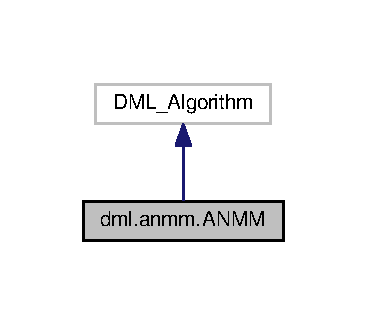
\includegraphics[width=176pt]{classdml_1_1anmm_1_1ANMM__inherit__graph}
\end{center}
\end{figure}


Collaboration diagram for dml.\+anmm.\+A\+N\+MM\+:
\nopagebreak
\begin{figure}[H]
\begin{center}
\leavevmode
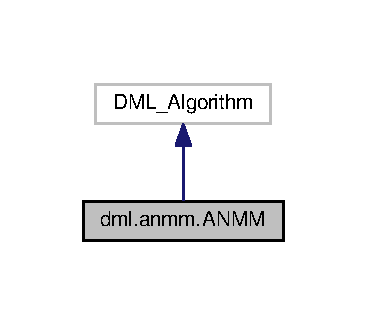
\includegraphics[width=176pt]{classdml_1_1anmm_1_1ANMM__coll__graph}
\end{center}
\end{figure}
\subsection*{Public Member Functions}
\begin{DoxyCompactItemize}
\item 
def {\bfseries \+\_\+\+\_\+init\+\_\+\+\_\+} (self, num\+\_\+dims=None, n\+\_\+friends=3, n\+\_\+enemies=1)\hypertarget{classdml_1_1anmm_1_1ANMM_abb2f1eacd76c294cd6bf76a8dcbfc388}{}\label{classdml_1_1anmm_1_1ANMM_abb2f1eacd76c294cd6bf76a8dcbfc388}

\item 
def \hyperlink{classdml_1_1anmm_1_1ANMM_a186d5fb3101c64747b75bdd5ae3f2ed5}{transformer} (self)
\item 
def \hyperlink{classdml_1_1anmm_1_1ANMM_af502f88ac840c080244c1d34e89f2aee}{metadata} (self)
\item 
def \hyperlink{classdml_1_1anmm_1_1ANMM_a251aa849680050f1e1a2af4e22bf6cbf}{fit} (self, X, y)
\end{DoxyCompactItemize}
\subsection*{Public Attributes}
\begin{DoxyCompactItemize}
\item 
{\bfseries num\+\_\+dims\+\_\+}\hypertarget{classdml_1_1anmm_1_1ANMM_a6771c7af15c0f0ea685bf5e9a50d328b}{}\label{classdml_1_1anmm_1_1ANMM_a6771c7af15c0f0ea685bf5e9a50d328b}

\item 
{\bfseries n\+\_\+fr\+\_\+}\hypertarget{classdml_1_1anmm_1_1ANMM_a5f7f7d727495d5b5d61079d8ea987aec}{}\label{classdml_1_1anmm_1_1ANMM_a5f7f7d727495d5b5d61079d8ea987aec}

\item 
{\bfseries n\+\_\+en\+\_\+}\hypertarget{classdml_1_1anmm_1_1ANMM_a574484da6b98ba391095ed32a6d236f7}{}\label{classdml_1_1anmm_1_1ANMM_a574484da6b98ba391095ed32a6d236f7}

\item 
{\bfseries acum\+\_\+eig\+\_\+}\hypertarget{classdml_1_1anmm_1_1ANMM_a080b8a5471764e8336ace0d404d20577}{}\label{classdml_1_1anmm_1_1ANMM_a080b8a5471764e8336ace0d404d20577}

\item 
{\bfseries nd\+\_\+}\hypertarget{classdml_1_1anmm_1_1ANMM_a9999e9c23bae79768264d109fa9dbd76}{}\label{classdml_1_1anmm_1_1ANMM_a9999e9c23bae79768264d109fa9dbd76}

\item 
{\bfseries y\+\_\+}\hypertarget{classdml_1_1anmm_1_1ANMM_aa24ad6ecac49e8dadd0eca14cfe3d51d}{}\label{classdml_1_1anmm_1_1ANMM_aa24ad6ecac49e8dadd0eca14cfe3d51d}

\item 
{\bfseries distance\+\_\+matrix\+\_\+}\hypertarget{classdml_1_1anmm_1_1ANMM_a423dc7ef50a3bca0f1d844b083e24e46}{}\label{classdml_1_1anmm_1_1ANMM_a423dc7ef50a3bca0f1d844b083e24e46}

\item 
{\bfseries d\+\_\+}\hypertarget{classdml_1_1anmm_1_1ANMM_a47ca72c3cb9642b1c2b103be3d25eb07}{}\label{classdml_1_1anmm_1_1ANMM_a47ca72c3cb9642b1c2b103be3d25eb07}

\item 
{\bfseries eig\+\_\+vecs\+\_\+}\hypertarget{classdml_1_1anmm_1_1ANMM_adc098f2b601d7eea1022187a17f89523}{}\label{classdml_1_1anmm_1_1ANMM_adc098f2b601d7eea1022187a17f89523}

\item 
{\bfseries eig\+\_\+pairs\+\_\+}\hypertarget{classdml_1_1anmm_1_1ANMM_aa2ef127bbf7a263cfbad5f02d55182c8}{}\label{classdml_1_1anmm_1_1ANMM_aa2ef127bbf7a263cfbad5f02d55182c8}

\item 
{\bfseries L\+\_\+}\hypertarget{classdml_1_1anmm_1_1ANMM_a655790def54adbb2cd503f1e974952a0}{}\label{classdml_1_1anmm_1_1ANMM_a655790def54adbb2cd503f1e974952a0}

\item 
{\bfseries acum\+\_\+eigvals\+\_\+}\hypertarget{classdml_1_1anmm_1_1ANMM_acab0aceabe6f76580aa8bc180c463376}{}\label{classdml_1_1anmm_1_1ANMM_acab0aceabe6f76580aa8bc180c463376}

\end{DoxyCompactItemize}


\subsection{Detailed Description}
\begin{DoxyVerb}Average Neighbor Margin Maximization (ANMM)

A DML Algorithm that obtains a transformer that maximizes the distance between the nearest friends and the nearest enemies for each example.

Parameters
----------
num_dims : int, default=None
    Dimension desired for the transformed data.

n_friends : int, default=3
    Number of nearest same-class neighbors to compute homogeneus neighborhood.

n_enemies : int, default=1
    Number of nearest different-class neighbors to compute heterogeneus neigborhood.

References
----------
    Fei Wang and Changshui Zhang. “Feature extraction by maximizing the average neighborhood
    margin”. In: Computer Vision and Pattern Recognition, 2007. CVPR’07. IEEE Conference on.
    IEEE. 2007, pages 1-8.
\end{DoxyVerb}
 

\subsection{Member Function Documentation}
\index{dml\+::anmm\+::\+A\+N\+MM@{dml\+::anmm\+::\+A\+N\+MM}!fit@{fit}}
\index{fit@{fit}!dml\+::anmm\+::\+A\+N\+MM@{dml\+::anmm\+::\+A\+N\+MM}}
\subsubsection[{\texorpdfstring{fit(self, X, y)}{fit(self, X, y)}}]{\setlength{\rightskip}{0pt plus 5cm}def dml.\+anmm.\+A\+N\+M\+M.\+fit (
\begin{DoxyParamCaption}
\item[{}]{self, }
\item[{}]{X, }
\item[{}]{y}
\end{DoxyParamCaption}
)}\hypertarget{classdml_1_1anmm_1_1ANMM_a251aa849680050f1e1a2af4e22bf6cbf}{}\label{classdml_1_1anmm_1_1ANMM_a251aa849680050f1e1a2af4e22bf6cbf}
\begin{DoxyVerb}Fit the model from the data in X and the labels in y.

Parameters
----------
X : array-like, shape (N x d)
    Training vector, where N is the number of samples, and d is the number of features.

y : array-like, shape (N)
    Labels vector, where N is the number of samples.

Returns
-------
self : object
    Returns the instance itself.
\end{DoxyVerb}
 \index{dml\+::anmm\+::\+A\+N\+MM@{dml\+::anmm\+::\+A\+N\+MM}!metadata@{metadata}}
\index{metadata@{metadata}!dml\+::anmm\+::\+A\+N\+MM@{dml\+::anmm\+::\+A\+N\+MM}}
\subsubsection[{\texorpdfstring{metadata(self)}{metadata(self)}}]{\setlength{\rightskip}{0pt plus 5cm}def dml.\+anmm.\+A\+N\+M\+M.\+metadata (
\begin{DoxyParamCaption}
\item[{}]{self}
\end{DoxyParamCaption}
)}\hypertarget{classdml_1_1anmm_1_1ANMM_af502f88ac840c080244c1d34e89f2aee}{}\label{classdml_1_1anmm_1_1ANMM_af502f88ac840c080244c1d34e89f2aee}
\begin{DoxyVerb}Obtains algorithm metadata.

Returns
-------
meta : A dictionary with the following metadata:
    acum_eig : eigenvalue rate accumulated in the learned output respect to the total dimension.

    num_dims : dimension of the reduced data.
\end{DoxyVerb}
 \index{dml\+::anmm\+::\+A\+N\+MM@{dml\+::anmm\+::\+A\+N\+MM}!transformer@{transformer}}
\index{transformer@{transformer}!dml\+::anmm\+::\+A\+N\+MM@{dml\+::anmm\+::\+A\+N\+MM}}
\subsubsection[{\texorpdfstring{transformer(self)}{transformer(self)}}]{\setlength{\rightskip}{0pt plus 5cm}def dml.\+anmm.\+A\+N\+M\+M.\+transformer (
\begin{DoxyParamCaption}
\item[{}]{self}
\end{DoxyParamCaption}
)}\hypertarget{classdml_1_1anmm_1_1ANMM_a186d5fb3101c64747b75bdd5ae3f2ed5}{}\label{classdml_1_1anmm_1_1ANMM_a186d5fb3101c64747b75bdd5ae3f2ed5}
\begin{DoxyVerb}Obtains the learned projection.

Returns
-------
L : (d'xd) matrix, where d' is the desired output dimension and d is the number of features.
\end{DoxyVerb}
 

The documentation for this class was generated from the following file\+:\begin{DoxyCompactItemize}
\item 
dml/anmm.\+pyx\end{DoxyCompactItemize}

\hypertarget{classdml_1_1dml__algorithm_1_1DML__Algorithm}{}\section{dml.\+dml\+\_\+algorithm.\+D\+M\+L\+\_\+\+Algorithm Class Reference}
\label{classdml_1_1dml__algorithm_1_1DML__Algorithm}\index{dml.\+dml\+\_\+algorithm.\+D\+M\+L\+\_\+\+Algorithm@{dml.\+dml\+\_\+algorithm.\+D\+M\+L\+\_\+\+Algorithm}}


Inheritance diagram for dml.\+dml\+\_\+algorithm.\+D\+M\+L\+\_\+\+Algorithm\+:\nopagebreak
\begin{figure}[H]
\begin{center}
\leavevmode
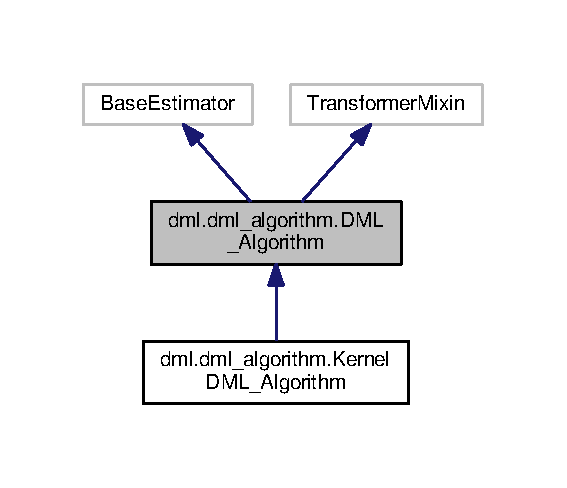
\includegraphics[width=272pt]{classdml_1_1dml__algorithm_1_1DML__Algorithm__inherit__graph}
\end{center}
\end{figure}


Collaboration diagram for dml.\+dml\+\_\+algorithm.\+D\+M\+L\+\_\+\+Algorithm\+:\nopagebreak
\begin{figure}[H]
\begin{center}
\leavevmode
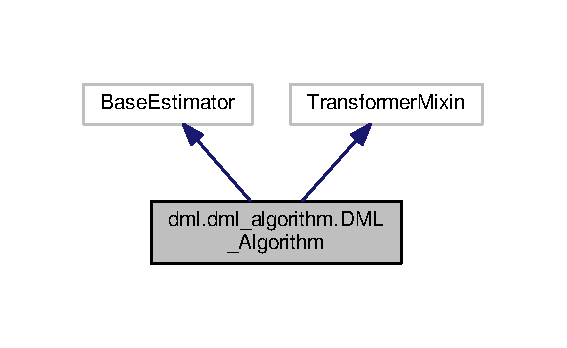
\includegraphics[width=272pt]{classdml_1_1dml__algorithm_1_1DML__Algorithm__coll__graph}
\end{center}
\end{figure}
\subsection*{Public Member Functions}
\begin{DoxyCompactItemize}
\item 
def {\bfseries \+\_\+\+\_\+init\+\_\+\+\_\+} (self)\hypertarget{classdml_1_1dml__algorithm_1_1DML__Algorithm_a3289181fb1120dedb754ef099cf61417}{}\label{classdml_1_1dml__algorithm_1_1DML__Algorithm_a3289181fb1120dedb754ef099cf61417}

\item 
def \hyperlink{classdml_1_1dml__algorithm_1_1DML__Algorithm_a9e344baf8028a0534b242de9c862d1c9}{metric} (self)
\item 
def \hyperlink{classdml_1_1dml__algorithm_1_1DML__Algorithm_a096525d92abf9242115c8f0a1d6f48d3}{transformer} (self)
\item 
def \hyperlink{classdml_1_1dml__algorithm_1_1DML__Algorithm_aa35480582eb941023ecce069496ed202}{transform} (self, X=None)
\item 
def {\bfseries metadata} (self)\hypertarget{classdml_1_1dml__algorithm_1_1DML__Algorithm_a639f5611375b5c11a92e931b1d45bb40}{}\label{classdml_1_1dml__algorithm_1_1DML__Algorithm_a639f5611375b5c11a92e931b1d45bb40}

\end{DoxyCompactItemize}
\subsection*{Public Attributes}
\begin{DoxyCompactItemize}
\item 
{\bfseries M\+\_\+}\hypertarget{classdml_1_1dml__algorithm_1_1DML__Algorithm_acb064d4924c9fb541d714931d8ff6a05}{}\label{classdml_1_1dml__algorithm_1_1DML__Algorithm_acb064d4924c9fb541d714931d8ff6a05}

\item 
{\bfseries L\+\_\+}\hypertarget{classdml_1_1dml__algorithm_1_1DML__Algorithm_adbd133f985a1296a0db3d9892057b0c2}{}\label{classdml_1_1dml__algorithm_1_1DML__Algorithm_adbd133f985a1296a0db3d9892057b0c2}

\end{DoxyCompactItemize}


\subsection{Detailed Description}
\begin{DoxyVerb}    Abstract class that defines a distance metric learning algorithm.
    Distance metric learning are implemented as subclasses of DML_Algorithm.
    A DML Algorithm can compute either a Mahalanobis metric matrix or an associated linear transformation.
    DML subclasses must override one of the following methods (metric or transformer), according to their computation way.
\end{DoxyVerb}
 

\subsection{Member Function Documentation}
\index{dml\+::dml\+\_\+algorithm\+::\+D\+M\+L\+\_\+\+Algorithm@{dml\+::dml\+\_\+algorithm\+::\+D\+M\+L\+\_\+\+Algorithm}!metric@{metric}}
\index{metric@{metric}!dml\+::dml\+\_\+algorithm\+::\+D\+M\+L\+\_\+\+Algorithm@{dml\+::dml\+\_\+algorithm\+::\+D\+M\+L\+\_\+\+Algorithm}}
\subsubsection[{\texorpdfstring{metric(self)}{metric(self)}}]{\setlength{\rightskip}{0pt plus 5cm}def dml.\+dml\+\_\+algorithm.\+D\+M\+L\+\_\+\+Algorithm.\+metric (
\begin{DoxyParamCaption}
\item[{}]{self}
\end{DoxyParamCaption}
)}\hypertarget{classdml_1_1dml__algorithm_1_1DML__Algorithm_a9e344baf8028a0534b242de9c862d1c9}{}\label{classdml_1_1dml__algorithm_1_1DML__Algorithm_a9e344baf8028a0534b242de9c862d1c9}
\begin{DoxyVerb}Computes the Mahalanobis matrix from the transformation matrix.
.. math:: M = L^T L

Returns
-------
M : (d x d) matrix. M defines a metric whose distace is given by
..math:: d(x,y) = \\sqrt{(x-y)^TM(x-y)}.
\end{DoxyVerb}
 \index{dml\+::dml\+\_\+algorithm\+::\+D\+M\+L\+\_\+\+Algorithm@{dml\+::dml\+\_\+algorithm\+::\+D\+M\+L\+\_\+\+Algorithm}!transform@{transform}}
\index{transform@{transform}!dml\+::dml\+\_\+algorithm\+::\+D\+M\+L\+\_\+\+Algorithm@{dml\+::dml\+\_\+algorithm\+::\+D\+M\+L\+\_\+\+Algorithm}}
\subsubsection[{\texorpdfstring{transform(self, X=\+None)}{transform(self, X=None)}}]{\setlength{\rightskip}{0pt plus 5cm}def dml.\+dml\+\_\+algorithm.\+D\+M\+L\+\_\+\+Algorithm.\+transform (
\begin{DoxyParamCaption}
\item[{}]{self, }
\item[{}]{X = {\ttfamily None}}
\end{DoxyParamCaption}
)}\hypertarget{classdml_1_1dml__algorithm_1_1DML__Algorithm_aa35480582eb941023ecce069496ed202}{}\label{classdml_1_1dml__algorithm_1_1DML__Algorithm_aa35480582eb941023ecce069496ed202}
\begin{DoxyVerb}Applies the metric transformation.

Parameters
----------
X : (N x d) matrix, optional
    Data to transform. If not supplied, the training data will be used.

Returns
-------
transformed : (N x d') matrix
    Input data transformed to the metric space by :math:`XL^{T}`
\end{DoxyVerb}
 \index{dml\+::dml\+\_\+algorithm\+::\+D\+M\+L\+\_\+\+Algorithm@{dml\+::dml\+\_\+algorithm\+::\+D\+M\+L\+\_\+\+Algorithm}!transformer@{transformer}}
\index{transformer@{transformer}!dml\+::dml\+\_\+algorithm\+::\+D\+M\+L\+\_\+\+Algorithm@{dml\+::dml\+\_\+algorithm\+::\+D\+M\+L\+\_\+\+Algorithm}}
\subsubsection[{\texorpdfstring{transformer(self)}{transformer(self)}}]{\setlength{\rightskip}{0pt plus 5cm}def dml.\+dml\+\_\+algorithm.\+D\+M\+L\+\_\+\+Algorithm.\+transformer (
\begin{DoxyParamCaption}
\item[{}]{self}
\end{DoxyParamCaption}
)}\hypertarget{classdml_1_1dml__algorithm_1_1DML__Algorithm_a096525d92abf9242115c8f0a1d6f48d3}{}\label{classdml_1_1dml__algorithm_1_1DML__Algorithm_a096525d92abf9242115c8f0a1d6f48d3}
\begin{DoxyVerb}Computes a transformation matrix from the Mahalanobis matrix.
..math:: L = M^{1/2}

Returns
-------
L : (d' x d) matrix, with d' <= d. It defines a projection. The distance can be calculated by
..math:: d(x,y) = \\|L(x-y)\\|_2.
\end{DoxyVerb}
 

The documentation for this class was generated from the following file\+:\begin{DoxyCompactItemize}
\item 
dml/dml\+\_\+algorithm.\+py\end{DoxyCompactItemize}

\hypertarget{classdml_1_1dml__eig_1_1DML__eig}{}\section{dml.\+dml\+\_\+eig.\+D\+M\+L\+\_\+eig Class Reference}
\label{classdml_1_1dml__eig_1_1DML__eig}\index{dml.\+dml\+\_\+eig.\+D\+M\+L\+\_\+eig@{dml.\+dml\+\_\+eig.\+D\+M\+L\+\_\+eig}}


Inheritance diagram for dml.\+dml\+\_\+eig.\+D\+M\+L\+\_\+eig\+:
\nopagebreak
\begin{figure}[H]
\begin{center}
\leavevmode
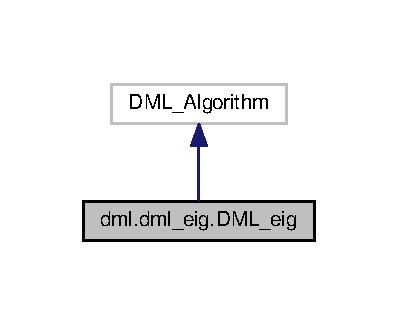
\includegraphics[width=191pt]{classdml_1_1dml__eig_1_1DML__eig__inherit__graph}
\end{center}
\end{figure}


Collaboration diagram for dml.\+dml\+\_\+eig.\+D\+M\+L\+\_\+eig\+:
\nopagebreak
\begin{figure}[H]
\begin{center}
\leavevmode
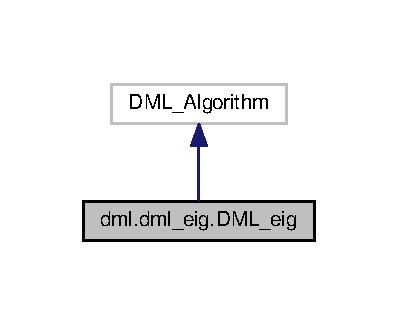
\includegraphics[width=191pt]{classdml_1_1dml__eig_1_1DML__eig__coll__graph}
\end{center}
\end{figure}
\subsection*{Public Member Functions}
\begin{DoxyCompactItemize}
\item 
def {\bfseries \+\_\+\+\_\+init\+\_\+\+\_\+} (self, mu=1e-\/4, tol=1e-\/5, eps=1e-\/10, max\+\_\+it=25)\hypertarget{classdml_1_1dml__eig_1_1DML__eig_a4571866c0c415246ba21a38e30367a6c}{}\label{classdml_1_1dml__eig_1_1DML__eig_a4571866c0c415246ba21a38e30367a6c}

\item 
def \hyperlink{classdml_1_1dml__eig_1_1DML__eig_af082539ea8c8d03f1115bfd21f73cd03}{metric} (self)
\item 
def \hyperlink{classdml_1_1dml__eig_1_1DML__eig_a59cfd79003d7a00ecfe3fbbf000bccf3}{metadata} (self)
\item 
def \hyperlink{classdml_1_1dml__eig_1_1DML__eig_a63a5d0661b8bc3a0dab73acb01df21ad}{fit} (self, X, y)
\end{DoxyCompactItemize}
\subsection*{Public Attributes}
\begin{DoxyCompactItemize}
\item 
{\bfseries mu\+\_\+}\hypertarget{classdml_1_1dml__eig_1_1DML__eig_a0c38272699780b875df613415b268013}{}\label{classdml_1_1dml__eig_1_1DML__eig_a0c38272699780b875df613415b268013}

\item 
{\bfseries tol\+\_\+}\hypertarget{classdml_1_1dml__eig_1_1DML__eig_adddb5a12cb8cd1e368734b802a145e6a}{}\label{classdml_1_1dml__eig_1_1DML__eig_adddb5a12cb8cd1e368734b802a145e6a}

\item 
{\bfseries max\+\_\+it\+\_\+}\hypertarget{classdml_1_1dml__eig_1_1DML__eig_a3b78ae9242b9388bc86bb5708bc12f0a}{}\label{classdml_1_1dml__eig_1_1DML__eig_a3b78ae9242b9388bc86bb5708bc12f0a}

\item 
{\bfseries eps\+\_\+}\hypertarget{classdml_1_1dml__eig_1_1DML__eig_a89ea7fd92bf0ae4126c5ae5dce591e3b}{}\label{classdml_1_1dml__eig_1_1DML__eig_a89ea7fd92bf0ae4126c5ae5dce591e3b}

\item 
{\bfseries initial\+\_\+error\+\_\+}\hypertarget{classdml_1_1dml__eig_1_1DML__eig_a1c45e608ba75f2f7401f58ac17a890ca}{}\label{classdml_1_1dml__eig_1_1DML__eig_a1c45e608ba75f2f7401f58ac17a890ca}

\item 
{\bfseries final\+\_\+error\+\_\+}\hypertarget{classdml_1_1dml__eig_1_1DML__eig_ad269c344871efe449035921b6c8d2e7d}{}\label{classdml_1_1dml__eig_1_1DML__eig_ad269c344871efe449035921b6c8d2e7d}

\item 
{\bfseries y\+\_\+}\hypertarget{classdml_1_1dml__eig_1_1DML__eig_a0a387b3d6b7612843e7a87be9a86260c}{}\label{classdml_1_1dml__eig_1_1DML__eig_a0a387b3d6b7612843e7a87be9a86260c}

\item 
{\bfseries M\+\_\+}\hypertarget{classdml_1_1dml__eig_1_1DML__eig_afe612921d74273029a54b7a7871a9dc9}{}\label{classdml_1_1dml__eig_1_1DML__eig_afe612921d74273029a54b7a7871a9dc9}

\end{DoxyCompactItemize}


\subsection{Detailed Description}
\begin{DoxyVerb}    Distance Metric Learning with Eigenvalue Optimization (DML-eig)

    A DML Algorithm that learns a metric that minimizes the minimum distance between different-class points
    constrained to the sum of distances at same-class points be non higher than a constant.

    Parameters
    ----------
    mu : float, default=1e-4
        Smoothing parameter.

    tol : float, default=1e-5
        Tolerance stop criterion (difference between two point iterations at gradient descent.)

    eps : float, default=1e-10
        Precision stop criterion (norm of gradient at gradient descent)

    max_it: int, default=25
        Number of iterations at gradient descent.

    References
    ----------
        Yiming Ying and Peng Li. “Distance metric learning with eigenvalue optimization”. In: Journal of
        Machine Learning Research 13.Jan (2012), pages 1-26.
\end{DoxyVerb}
 

\subsection{Member Function Documentation}
\index{dml\+::dml\+\_\+eig\+::\+D\+M\+L\+\_\+eig@{dml\+::dml\+\_\+eig\+::\+D\+M\+L\+\_\+eig}!fit@{fit}}
\index{fit@{fit}!dml\+::dml\+\_\+eig\+::\+D\+M\+L\+\_\+eig@{dml\+::dml\+\_\+eig\+::\+D\+M\+L\+\_\+eig}}
\subsubsection[{\texorpdfstring{fit(self, X, y)}{fit(self, X, y)}}]{\setlength{\rightskip}{0pt plus 5cm}def dml.\+dml\+\_\+eig.\+D\+M\+L\+\_\+eig.\+fit (
\begin{DoxyParamCaption}
\item[{}]{self, }
\item[{}]{X, }
\item[{}]{y}
\end{DoxyParamCaption}
)}\hypertarget{classdml_1_1dml__eig_1_1DML__eig_a63a5d0661b8bc3a0dab73acb01df21ad}{}\label{classdml_1_1dml__eig_1_1DML__eig_a63a5d0661b8bc3a0dab73acb01df21ad}
\begin{DoxyVerb}Fit the model from the data in X and the labels in y.

Parameters
----------
X : array-like, shape (N x d)
    Training vector, where N is the number of samples, and d is the number of features.

y : array-like, shape (N)
    Labels vector, where N is the number of samples.

Returns
-------
self : object
    Returns the instance itself.
\end{DoxyVerb}
\begin{DoxyVerb}# Initialize parameters
X, y = check_X_y(X,y)
self.X_, self.y_ = X,y

S, D = DML_eig._label_to_similarity_set(y)

mu = self.mu_
beta = self.beta_
tol = self.tol_
max_it = self.max_it_
eps = self.eps_
linesearch = self.linesearch_

ns, nd = S.shape[0], D.shape[0]
n, d = X.shape

Xt = np.zeros([d*d,nd])
ut = np.ones([ns,1])
XS = DML_eig._SODW(X.T,S[:,0],S[:,1],ut)

XS = (XS + XS.T)/2.0

Sig, U = eig(XS);
Sig = np.real(Sig)
Sig[Sig <= eps]=0.0
XSL = U.dot(np.diag(np.sqrt(Sig))).dot(U.T)

invXS = pinv(XS)
XXtr = pinv(XSL).dot(X.T)

for i in xrange(nd):
    temp1 = (XXtr[:,D[i,1]]-XXtr[:,D[i,0]]).dot((XXtr[:,D[i,1]]-XXtr[:,D[i,0]]).T)
    Xt[:,i] = temp1

Id = np.eye(d)
MM = Id[:,1].dot(Id[1,:])

count=True
its=0
fval=[]
change_fval=[]
change_M=[]
mu = mu/np.log(nd)

while its < max_it and count:
    temp = -Xt.T.dot(MM)/mu

    mg = np.max(temp)
    a = np.exp(temp-mg)
    print(Xt.shape,a.shape)
    gradfM = np.reshape((Xt.dot(a))/np.sum(a),[d,d])-beta*invXS
    gradfM = (gradfM + gradfM.T)/2.0
    fval.append(-mu*(np.log(np.sum(a))+mg))

    # Compute largest eigenvalue
    dd, V = eig(gradfM)
    V = V[:,np.argsort(dd)[::-1]]
    V=V[:,0]

    SM = V.dot(V.T)

    MMp = MM
    pd = SM - MMp

    if linesearch:
line_tol = 1e-3
alphak = 1/(its+1)
max_linesearch=10
linesearch_iter = 1
flag_linesearch = True

while flag_linesearch and linesearch_iter <= max_linesearch:
    MM = MMp + alphak*pd

    temp = - Xt.T.dot(MM)/mu
    temp[temp < -700] = -700
    temp[temp > 700] = 700
    mg = np.max(temp)
    a = np.exp(temp-mg)
    tempfval = -mu*(np.log(np.sum(a))+mg)
    ftaylor = fval[-1]+alphak*line_tol*np.trace(gradfM.dot(pd))

    if tempfval >= ftaylor:
        flag_linesearch=False
    else:
        alphak = alphak/2
    linesearch_iter += 1
    else:
alphak = 2/(its+2)
MM = MMp+alphak*pd
#change_M.append(np.sqrt(np.sum((MM-MMp)*(MM-MMp))))

    if its > 1:
change_fval.append(np.abs(fval[-1]-fval[-2])/np.abs(fval[-1]+eps))
if change_fval[-1] < tol:
    count=False

    its += 1
\end{DoxyVerb}
 \index{dml\+::dml\+\_\+eig\+::\+D\+M\+L\+\_\+eig@{dml\+::dml\+\_\+eig\+::\+D\+M\+L\+\_\+eig}!metadata@{metadata}}
\index{metadata@{metadata}!dml\+::dml\+\_\+eig\+::\+D\+M\+L\+\_\+eig@{dml\+::dml\+\_\+eig\+::\+D\+M\+L\+\_\+eig}}
\subsubsection[{\texorpdfstring{metadata(self)}{metadata(self)}}]{\setlength{\rightskip}{0pt plus 5cm}def dml.\+dml\+\_\+eig.\+D\+M\+L\+\_\+eig.\+metadata (
\begin{DoxyParamCaption}
\item[{}]{self}
\end{DoxyParamCaption}
)}\hypertarget{classdml_1_1dml__eig_1_1DML__eig_a59cfd79003d7a00ecfe3fbbf000bccf3}{}\label{classdml_1_1dml__eig_1_1DML__eig_a59cfd79003d7a00ecfe3fbbf000bccf3}
\begin{DoxyVerb}Obtains algorithm metadata.

Returns
-------
meta : A dictionary with the following metadata:
    initial_error : initial value of the objective error function.

    final_error : final value of the objective error function.
\end{DoxyVerb}
 \index{dml\+::dml\+\_\+eig\+::\+D\+M\+L\+\_\+eig@{dml\+::dml\+\_\+eig\+::\+D\+M\+L\+\_\+eig}!metric@{metric}}
\index{metric@{metric}!dml\+::dml\+\_\+eig\+::\+D\+M\+L\+\_\+eig@{dml\+::dml\+\_\+eig\+::\+D\+M\+L\+\_\+eig}}
\subsubsection[{\texorpdfstring{metric(self)}{metric(self)}}]{\setlength{\rightskip}{0pt plus 5cm}def dml.\+dml\+\_\+eig.\+D\+M\+L\+\_\+eig.\+metric (
\begin{DoxyParamCaption}
\item[{}]{self}
\end{DoxyParamCaption}
)}\hypertarget{classdml_1_1dml__eig_1_1DML__eig_af082539ea8c8d03f1115bfd21f73cd03}{}\label{classdml_1_1dml__eig_1_1DML__eig_af082539ea8c8d03f1115bfd21f73cd03}
\begin{DoxyVerb}Obtains the learned metric.

Returns
-------
M : (dxd) positive semidefinite matrix, where d is the number of features.
\end{DoxyVerb}
 

The documentation for this class was generated from the following file\+:\begin{DoxyCompactItemize}
\item 
dml/dml\+\_\+eig.\+pyx\end{DoxyCompactItemize}

\hypertarget{classdml_1_1dmlmj_1_1DMLMJ}{}\section{dml.\+dmlmj.\+D\+M\+L\+MJ Class Reference}
\label{classdml_1_1dmlmj_1_1DMLMJ}\index{dml.\+dmlmj.\+D\+M\+L\+MJ@{dml.\+dmlmj.\+D\+M\+L\+MJ}}


Inheritance diagram for dml.\+dmlmj.\+D\+M\+L\+MJ\+:
\nopagebreak
\begin{figure}[H]
\begin{center}
\leavevmode
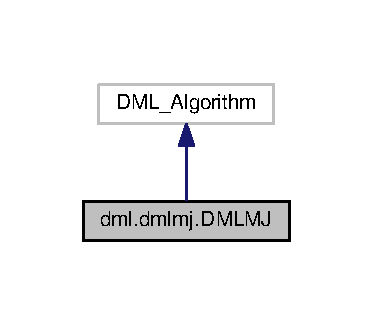
\includegraphics[width=179pt]{classdml_1_1dmlmj_1_1DMLMJ__inherit__graph}
\end{center}
\end{figure}


Collaboration diagram for dml.\+dmlmj.\+D\+M\+L\+MJ\+:
\nopagebreak
\begin{figure}[H]
\begin{center}
\leavevmode
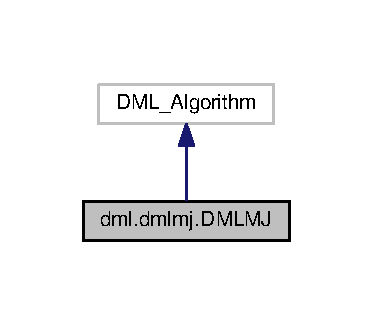
\includegraphics[width=179pt]{classdml_1_1dmlmj_1_1DMLMJ__coll__graph}
\end{center}
\end{figure}
\subsection*{Public Member Functions}
\begin{DoxyCompactItemize}
\item 
def {\bfseries \+\_\+\+\_\+init\+\_\+\+\_\+} (self, num\+\_\+dims=None, n\+\_\+neighbors=3, alpha=0.\+001, reg\+\_\+tol=1e-\/10)\hypertarget{classdml_1_1dmlmj_1_1DMLMJ_a5bc22f7adee1aff574db36f7a4c3cc08}{}\label{classdml_1_1dmlmj_1_1DMLMJ_a5bc22f7adee1aff574db36f7a4c3cc08}

\item 
def \hyperlink{classdml_1_1dmlmj_1_1DMLMJ_a025017cae3f8607f6a28c116f1505b4e}{transformer} (self)
\item 
def \hyperlink{classdml_1_1dmlmj_1_1DMLMJ_a9747589a8736d994b0e2af00ea92d3eb}{metadata} (self)
\item 
def \hyperlink{classdml_1_1dmlmj_1_1DMLMJ_ada35e252dc232294ad3ef830f5f5fc1e}{fit} (self, X, y)
\end{DoxyCompactItemize}
\subsection*{Public Attributes}
\begin{DoxyCompactItemize}
\item 
{\bfseries num\+\_\+dims\+\_\+}\hypertarget{classdml_1_1dmlmj_1_1DMLMJ_ace12122bfac7d41adc966f9e302ea71a}{}\label{classdml_1_1dmlmj_1_1DMLMJ_ace12122bfac7d41adc966f9e302ea71a}

\item 
{\bfseries k\+\_\+}\hypertarget{classdml_1_1dmlmj_1_1DMLMJ_a8475b2879d93be3f8fc8daf25e346170}{}\label{classdml_1_1dmlmj_1_1DMLMJ_a8475b2879d93be3f8fc8daf25e346170}

\item 
{\bfseries alpha\+\_\+}\hypertarget{classdml_1_1dmlmj_1_1DMLMJ_ab7673494f9eb745913bc4438de7eeddc}{}\label{classdml_1_1dmlmj_1_1DMLMJ_ab7673494f9eb745913bc4438de7eeddc}

\item 
{\bfseries reg\+\_\+tol\+\_\+}\hypertarget{classdml_1_1dmlmj_1_1DMLMJ_a113677d13351af6d9eb9d7775315d33c}{}\label{classdml_1_1dmlmj_1_1DMLMJ_a113677d13351af6d9eb9d7775315d33c}

\item 
{\bfseries acum\+\_\+eig\+\_\+}\hypertarget{classdml_1_1dmlmj_1_1DMLMJ_a903e254c6b27dff75b80f8907867a1da}{}\label{classdml_1_1dmlmj_1_1DMLMJ_a903e254c6b27dff75b80f8907867a1da}

\item 
{\bfseries nd\+\_\+}\hypertarget{classdml_1_1dmlmj_1_1DMLMJ_a7131d8cd3da3f7a22a540451ba784788}{}\label{classdml_1_1dmlmj_1_1DMLMJ_a7131d8cd3da3f7a22a540451ba784788}

\item 
{\bfseries y\+\_\+}\hypertarget{classdml_1_1dmlmj_1_1DMLMJ_a0674651b8d68e5d58a8f39d09c0bf294}{}\label{classdml_1_1dmlmj_1_1DMLMJ_a0674651b8d68e5d58a8f39d09c0bf294}

\item 
{\bfseries d\+\_\+}\hypertarget{classdml_1_1dmlmj_1_1DMLMJ_aa688cb13ffb4651f6b02b0801b372dc4}{}\label{classdml_1_1dmlmj_1_1DMLMJ_aa688cb13ffb4651f6b02b0801b372dc4}

\item 
{\bfseries eig\+\_\+vecs\+\_\+}\hypertarget{classdml_1_1dmlmj_1_1DMLMJ_adaf9dea0e690fd3489cc98e429b15854}{}\label{classdml_1_1dmlmj_1_1DMLMJ_adaf9dea0e690fd3489cc98e429b15854}

\item 
{\bfseries eig\+\_\+pairs\+\_\+}\hypertarget{classdml_1_1dmlmj_1_1DMLMJ_ae6ff2fcdb2602369ab26cf708ce5afab}{}\label{classdml_1_1dmlmj_1_1DMLMJ_ae6ff2fcdb2602369ab26cf708ce5afab}

\item 
{\bfseries L\+\_\+}\hypertarget{classdml_1_1dmlmj_1_1DMLMJ_ac7c18f71ee66f4e647d4b97406fb2678}{}\label{classdml_1_1dmlmj_1_1DMLMJ_ac7c18f71ee66f4e647d4b97406fb2678}

\item 
{\bfseries acum\+\_\+eigvals\+\_\+}\hypertarget{classdml_1_1dmlmj_1_1DMLMJ_a1e5ee7e4b101147871a86bdc4fd168dd}{}\label{classdml_1_1dmlmj_1_1DMLMJ_a1e5ee7e4b101147871a86bdc4fd168dd}

\end{DoxyCompactItemize}


\subsection{Detailed Description}
\begin{DoxyVerb}Distance Metric Learning through the Maximization of the Jeffrey divergence (DMLMJ).

A DML Algorithm that obtains a transformer that maximizes the Jeffrey divergence between
the distribution of differences of same-class neighbors and the distribution of differences between
different-class neighbors.

Parameters
----------
num_dims : int, default=None
    Dimension desired for the transformed data.

n_neighbors : int, default=3
    Number of neighbors to consider in the computation of the difference spaces.

alpha : float, default=0.001
    Regularization parameter for inverse matrix computation.

reg_tol : float, default=1e-10
    Tolerance threshold for applying regularization. The tolerance is compared with the matrix determinant.

References
----------
    Bac Nguyen, Carlos Morell and Bernard De Baets. “Supervised distance metric learning through
    maximization of the Jeffrey divergence”. In: Pattern Recognition 64 (2017), pages 215-225.
\end{DoxyVerb}
 

\subsection{Member Function Documentation}
\index{dml\+::dmlmj\+::\+D\+M\+L\+MJ@{dml\+::dmlmj\+::\+D\+M\+L\+MJ}!fit@{fit}}
\index{fit@{fit}!dml\+::dmlmj\+::\+D\+M\+L\+MJ@{dml\+::dmlmj\+::\+D\+M\+L\+MJ}}
\subsubsection[{\texorpdfstring{fit(self, X, y)}{fit(self, X, y)}}]{\setlength{\rightskip}{0pt plus 5cm}def dml.\+dmlmj.\+D\+M\+L\+M\+J.\+fit (
\begin{DoxyParamCaption}
\item[{}]{self, }
\item[{}]{X, }
\item[{}]{y}
\end{DoxyParamCaption}
)}\hypertarget{classdml_1_1dmlmj_1_1DMLMJ_ada35e252dc232294ad3ef830f5f5fc1e}{}\label{classdml_1_1dmlmj_1_1DMLMJ_ada35e252dc232294ad3ef830f5f5fc1e}
\begin{DoxyVerb}Fit the model from the data in X and the labels in y.

Parameters
----------
X : array-like, shape (N x d)
    Training vector, where N is the number of samples, and d is the number of features.

y : array-like, shape (N)
    Labels vector, where N is the number of samples.

Returns
-------
self : object
    Returns the instance itself.
\end{DoxyVerb}
 \index{dml\+::dmlmj\+::\+D\+M\+L\+MJ@{dml\+::dmlmj\+::\+D\+M\+L\+MJ}!metadata@{metadata}}
\index{metadata@{metadata}!dml\+::dmlmj\+::\+D\+M\+L\+MJ@{dml\+::dmlmj\+::\+D\+M\+L\+MJ}}
\subsubsection[{\texorpdfstring{metadata(self)}{metadata(self)}}]{\setlength{\rightskip}{0pt plus 5cm}def dml.\+dmlmj.\+D\+M\+L\+M\+J.\+metadata (
\begin{DoxyParamCaption}
\item[{}]{self}
\end{DoxyParamCaption}
)}\hypertarget{classdml_1_1dmlmj_1_1DMLMJ_a9747589a8736d994b0e2af00ea92d3eb}{}\label{classdml_1_1dmlmj_1_1DMLMJ_a9747589a8736d994b0e2af00ea92d3eb}
\begin{DoxyVerb}Obtains algorithm metadata.

Returns
-------
meta : A dictionary with the following metadata:
    acum_eig : eigenvalue rate accumulated in the learned output respect to the total dimension.

    num_dims : dimension of the reduced data.
\end{DoxyVerb}
 \index{dml\+::dmlmj\+::\+D\+M\+L\+MJ@{dml\+::dmlmj\+::\+D\+M\+L\+MJ}!transformer@{transformer}}
\index{transformer@{transformer}!dml\+::dmlmj\+::\+D\+M\+L\+MJ@{dml\+::dmlmj\+::\+D\+M\+L\+MJ}}
\subsubsection[{\texorpdfstring{transformer(self)}{transformer(self)}}]{\setlength{\rightskip}{0pt plus 5cm}def dml.\+dmlmj.\+D\+M\+L\+M\+J.\+transformer (
\begin{DoxyParamCaption}
\item[{}]{self}
\end{DoxyParamCaption}
)}\hypertarget{classdml_1_1dmlmj_1_1DMLMJ_a025017cae3f8607f6a28c116f1505b4e}{}\label{classdml_1_1dmlmj_1_1DMLMJ_a025017cae3f8607f6a28c116f1505b4e}
\begin{DoxyVerb}Obtains the learned projection.

Returns
-------
L : (d'xd) matrix, where d' is the desired output dimension and d is the number of features.
\end{DoxyVerb}
 

The documentation for this class was generated from the following file\+:\begin{DoxyCompactItemize}
\item 
dml/dmlmj.\+pyx\end{DoxyCompactItemize}

\hypertarget{classdml_1_1base_1_1Euclidean}{}\section{dml.\+base.\+Euclidean Class Reference}
\label{classdml_1_1base_1_1Euclidean}\index{dml.\+base.\+Euclidean@{dml.\+base.\+Euclidean}}


Inheritance diagram for dml.\+base.\+Euclidean\+:\nopagebreak
\begin{figure}[H]
\begin{center}
\leavevmode
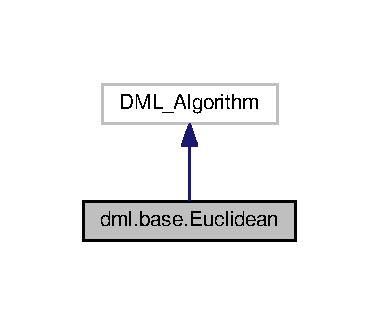
\includegraphics[width=182pt]{classdml_1_1base_1_1Euclidean__inherit__graph}
\end{center}
\end{figure}


Collaboration diagram for dml.\+base.\+Euclidean\+:\nopagebreak
\begin{figure}[H]
\begin{center}
\leavevmode
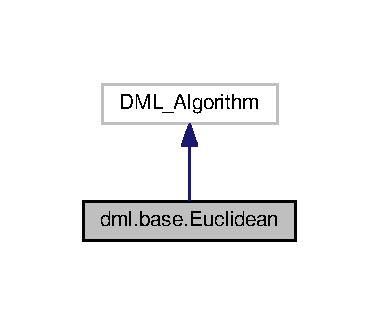
\includegraphics[width=182pt]{classdml_1_1base_1_1Euclidean__coll__graph}
\end{center}
\end{figure}
\subsection*{Public Member Functions}
\begin{DoxyCompactItemize}
\item 
def {\bfseries \+\_\+\+\_\+init\+\_\+\+\_\+} (self)\hypertarget{classdml_1_1base_1_1Euclidean_a2d007bd1fc23843cdfe254ab324430ee}{}\label{classdml_1_1base_1_1Euclidean_a2d007bd1fc23843cdfe254ab324430ee}

\item 
def \hyperlink{classdml_1_1base_1_1Euclidean_abb5019bfc4f36264956a35134bb70ead}{fit} (self, X, y)
\item 
def \hyperlink{classdml_1_1base_1_1Euclidean_aaf850e3fb2714fddaae16930f2a0384c}{transformer} (self)
\item 
def \hyperlink{classdml_1_1base_1_1Euclidean_a476fc37bc38eaa15b3de0dead8e4ba63}{metric} (self)
\item 
def \hyperlink{classdml_1_1base_1_1Euclidean_a5b8e56f02ab4c981cf4bc71fddf7acdb}{transform} (self, X=None)
\end{DoxyCompactItemize}
\subsection*{Public Attributes}
\begin{DoxyCompactItemize}
\item 
{\bfseries X\+\_\+}\hypertarget{classdml_1_1base_1_1Euclidean_a93e7d1dde6c572e5ab42d575d626e030}{}\label{classdml_1_1base_1_1Euclidean_a93e7d1dde6c572e5ab42d575d626e030}

\item 
{\bfseries I\+\_\+}\hypertarget{classdml_1_1base_1_1Euclidean_aeac6e6927daad328db69450880ce04cb}{}\label{classdml_1_1base_1_1Euclidean_aeac6e6927daad328db69450880ce04cb}

\end{DoxyCompactItemize}


\subsection{Detailed Description}
\begin{DoxyVerb}A basic transformer that represents the euclidean distance.
\end{DoxyVerb}
 

\subsection{Member Function Documentation}
\index{dml\+::base\+::\+Euclidean@{dml\+::base\+::\+Euclidean}!fit@{fit}}
\index{fit@{fit}!dml\+::base\+::\+Euclidean@{dml\+::base\+::\+Euclidean}}
\subsubsection[{\texorpdfstring{fit(self, X, y)}{fit(self, X, y)}}]{\setlength{\rightskip}{0pt plus 5cm}def dml.\+base.\+Euclidean.\+fit (
\begin{DoxyParamCaption}
\item[{}]{self, }
\item[{}]{X, }
\item[{}]{y}
\end{DoxyParamCaption}
)}\hypertarget{classdml_1_1base_1_1Euclidean_abb5019bfc4f36264956a35134bb70ead}{}\label{classdml_1_1base_1_1Euclidean_abb5019bfc4f36264956a35134bb70ead}
\begin{DoxyVerb}Fit the model from the data in X and the labels in y.

Parameters
----------
X : array-like, shape (N x d)
    Training vector, where N is the number of samples, and d is the number of features.

y : array-like, shape (N)
    Labels vector, where N is the number of samples.

Returns
-------
self : object
    Returns the instance itself.
\end{DoxyVerb}
 \index{dml\+::base\+::\+Euclidean@{dml\+::base\+::\+Euclidean}!metric@{metric}}
\index{metric@{metric}!dml\+::base\+::\+Euclidean@{dml\+::base\+::\+Euclidean}}
\subsubsection[{\texorpdfstring{metric(self)}{metric(self)}}]{\setlength{\rightskip}{0pt plus 5cm}def dml.\+base.\+Euclidean.\+metric (
\begin{DoxyParamCaption}
\item[{}]{self}
\end{DoxyParamCaption}
)}\hypertarget{classdml_1_1base_1_1Euclidean_a476fc37bc38eaa15b3de0dead8e4ba63}{}\label{classdml_1_1base_1_1Euclidean_a476fc37bc38eaa15b3de0dead8e4ba63}
\begin{DoxyVerb}Obtains the learned metric.

Returns
-------
M : (dxd) positive semidefinite matrix, where d is the number of features.
\end{DoxyVerb}
 \index{dml\+::base\+::\+Euclidean@{dml\+::base\+::\+Euclidean}!transform@{transform}}
\index{transform@{transform}!dml\+::base\+::\+Euclidean@{dml\+::base\+::\+Euclidean}}
\subsubsection[{\texorpdfstring{transform(self, X=\+None)}{transform(self, X=None)}}]{\setlength{\rightskip}{0pt plus 5cm}def dml.\+base.\+Euclidean.\+transform (
\begin{DoxyParamCaption}
\item[{}]{self, }
\item[{}]{X = {\ttfamily None}}
\end{DoxyParamCaption}
)}\hypertarget{classdml_1_1base_1_1Euclidean_a5b8e56f02ab4c981cf4bc71fddf7acdb}{}\label{classdml_1_1base_1_1Euclidean_a5b8e56f02ab4c981cf4bc71fddf7acdb}
\begin{DoxyVerb}Applies the metric transformation.

Parameters
----------
X : (N x d) matrix, optional
    Data to transform. If not supplied, the training data will be used.

Returns
-------
transformed : (N x d') matrix
    Input data transformed to the metric space by :math:`XL^{\\top}`
\end{DoxyVerb}
 \index{dml\+::base\+::\+Euclidean@{dml\+::base\+::\+Euclidean}!transformer@{transformer}}
\index{transformer@{transformer}!dml\+::base\+::\+Euclidean@{dml\+::base\+::\+Euclidean}}
\subsubsection[{\texorpdfstring{transformer(self)}{transformer(self)}}]{\setlength{\rightskip}{0pt plus 5cm}def dml.\+base.\+Euclidean.\+transformer (
\begin{DoxyParamCaption}
\item[{}]{self}
\end{DoxyParamCaption}
)}\hypertarget{classdml_1_1base_1_1Euclidean_aaf850e3fb2714fddaae16930f2a0384c}{}\label{classdml_1_1base_1_1Euclidean_aaf850e3fb2714fddaae16930f2a0384c}
\begin{DoxyVerb}Obtains the learned projection.

Returns
-------
L : (d'xd) matrix, where d' is the desired output dimension and d is the number of features.
\end{DoxyVerb}
 

The documentation for this class was generated from the following file\+:\begin{DoxyCompactItemize}
\item 
dml/base.\+py\end{DoxyCompactItemize}

\hypertarget{classdml_1_1itml_1_1ITML}{}\section{dml.\+itml.\+I\+T\+ML Class Reference}
\label{classdml_1_1itml_1_1ITML}\index{dml.\+itml.\+I\+T\+ML@{dml.\+itml.\+I\+T\+ML}}


Inheritance diagram for dml.\+itml.\+I\+T\+ML\+:
\nopagebreak
\begin{figure}[H]
\begin{center}
\leavevmode
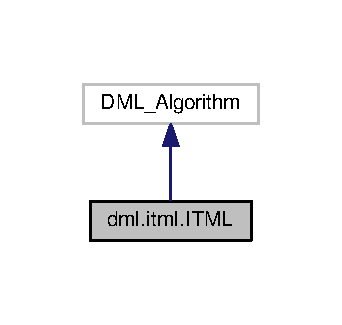
\includegraphics[width=164pt]{classdml_1_1itml_1_1ITML__inherit__graph}
\end{center}
\end{figure}


Collaboration diagram for dml.\+itml.\+I\+T\+ML\+:
\nopagebreak
\begin{figure}[H]
\begin{center}
\leavevmode
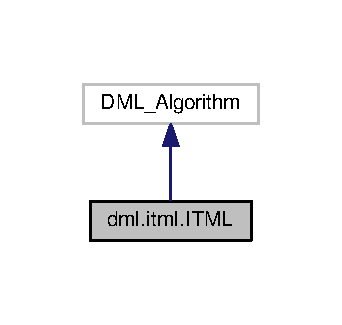
\includegraphics[width=164pt]{classdml_1_1itml_1_1ITML__coll__graph}
\end{center}
\end{figure}
\subsection*{Public Member Functions}
\begin{DoxyCompactItemize}
\item 
def {\bfseries \+\_\+\+\_\+init\+\_\+\+\_\+} (self, initial\+\_\+metric=None, upper\+\_\+bound=None, lower\+\_\+bound=None, num\+\_\+constraints=None, gamma=1.\+0, tol=0.\+001, max\+\_\+iter=100000, low\+\_\+perc=5, up\+\_\+perc=95)\hypertarget{classdml_1_1itml_1_1ITML_adf50511395db38402d68aeb8d4c8bc95}{}\label{classdml_1_1itml_1_1ITML_adf50511395db38402d68aeb8d4c8bc95}

\item 
def \hyperlink{classdml_1_1itml_1_1ITML_abbd45935d0afe4701144295ef869b9f0}{metric} (self)
\item 
def \hyperlink{classdml_1_1itml_1_1ITML_aec44a9262788d7af9b250fbab7b6e7d5}{fit} (self, X, y)
\end{DoxyCompactItemize}
\subsection*{Public Attributes}
\begin{DoxyCompactItemize}
\item 
{\bfseries M0\+\_\+}\hypertarget{classdml_1_1itml_1_1ITML_ac63b64b8a3e5849d1aa40515da7c130a}{}\label{classdml_1_1itml_1_1ITML_ac63b64b8a3e5849d1aa40515da7c130a}

\item 
{\bfseries u\+\_\+}\hypertarget{classdml_1_1itml_1_1ITML_a2559a6344d9b47f47be9c024e4c270da}{}\label{classdml_1_1itml_1_1ITML_a2559a6344d9b47f47be9c024e4c270da}

\item 
{\bfseries l\+\_\+}\hypertarget{classdml_1_1itml_1_1ITML_ad1a709f43ab7917786fb37dc0183df18}{}\label{classdml_1_1itml_1_1ITML_ad1a709f43ab7917786fb37dc0183df18}

\item 
{\bfseries gamma\+\_\+}\hypertarget{classdml_1_1itml_1_1ITML_a462e86708d6b624927f183c48c02ab20}{}\label{classdml_1_1itml_1_1ITML_a462e86708d6b624927f183c48c02ab20}

\item 
{\bfseries tol\+\_\+}\hypertarget{classdml_1_1itml_1_1ITML_a2857fc8ddbb10097dfadb1e2dbf2cab0}{}\label{classdml_1_1itml_1_1ITML_a2857fc8ddbb10097dfadb1e2dbf2cab0}

\item 
{\bfseries max\+\_\+its\+\_\+}\hypertarget{classdml_1_1itml_1_1ITML_a8b9d300bb398e3697600962a6fd01e97}{}\label{classdml_1_1itml_1_1ITML_a8b9d300bb398e3697600962a6fd01e97}

\item 
{\bfseries num\+\_\+constraints\+\_\+}\hypertarget{classdml_1_1itml_1_1ITML_ab09ecc18c6f9541a2a600bb83515eac0}{}\label{classdml_1_1itml_1_1ITML_ab09ecc18c6f9541a2a600bb83515eac0}

\item 
{\bfseries low\+\_\+perc\+\_\+}\hypertarget{classdml_1_1itml_1_1ITML_a6f1d95e6bb791cda7767bced1cea6e04}{}\label{classdml_1_1itml_1_1ITML_a6f1d95e6bb791cda7767bced1cea6e04}

\item 
{\bfseries up\+\_\+perc\+\_\+}\hypertarget{classdml_1_1itml_1_1ITML_adb79e10a9be631ffceb4db710b22c36c}{}\label{classdml_1_1itml_1_1ITML_adb79e10a9be631ffceb4db710b22c36c}

\item 
{\bfseries y\+\_\+}\hypertarget{classdml_1_1itml_1_1ITML_ad2d395296275aecfe8e38ec8f71e6cc4}{}\label{classdml_1_1itml_1_1ITML_ad2d395296275aecfe8e38ec8f71e6cc4}

\item 
{\bfseries M\+\_\+}\hypertarget{classdml_1_1itml_1_1ITML_a240b13a953d229f22a31431ec39eeaf3}{}\label{classdml_1_1itml_1_1ITML_a240b13a953d229f22a31431ec39eeaf3}

\end{DoxyCompactItemize}


\subsection{Detailed Description}
\begin{DoxyVerb}Information Theoretic Metric Learning (ITML).

A DML algorithm that learns a metric associated to the nearest gaussian distribution satisfying similarity constraints.
The nearest gaussian distribution is obtained minimizing the Kullback-Leibler divergence.

Parameters
----------

initial_metric : 2D-Array or Matrix

        A positive definite matrix that defines the initial metric used to compare.

upper_bound : float, default=None

        Bound for dissimilarity constraints. If None, it will be estimated from upper_perc.

lower_bound : float, default=None

        Bound for similarity constraints. If None, it will be estimated from lower_perc.

num_constraints : int, default=None

        Number of constraints to generate. If None, it will be taken as 40 * k * (k-1), where k is the number of classes.

gamma : float, default=1.0

        The gamma value for slack variables.

tol : float, default=0.001

        Tolerance stop criterion for the algorithm.

max_iter : int, default=100000

        Maximum number of iterations for the algorithm.

low_perc : int, default=5

        Lower percentile (from 0 to 100) to estimate the lower bound from the dataset. Ignored if lower_bound is provided.

up_perc : int, default=95

        Upper percentile (from 0 to 100) to estimate the upper bound from the dataset. Ignored if upper_bound is provided.

References
----------
    Jason V Davis et al. “Information-theoretic metric learning”. In: Proceedings of the 24th
    international conference on Machine learning. ACM. 2007, pages. 209-216.\end{DoxyVerb}
 

\subsection{Member Function Documentation}
\index{dml\+::itml\+::\+I\+T\+ML@{dml\+::itml\+::\+I\+T\+ML}!fit@{fit}}
\index{fit@{fit}!dml\+::itml\+::\+I\+T\+ML@{dml\+::itml\+::\+I\+T\+ML}}
\subsubsection[{\texorpdfstring{fit(self, X, y)}{fit(self, X, y)}}]{\setlength{\rightskip}{0pt plus 5cm}def dml.\+itml.\+I\+T\+M\+L.\+fit (
\begin{DoxyParamCaption}
\item[{}]{self, }
\item[{}]{X, }
\item[{}]{y}
\end{DoxyParamCaption}
)}\hypertarget{classdml_1_1itml_1_1ITML_aec44a9262788d7af9b250fbab7b6e7d5}{}\label{classdml_1_1itml_1_1ITML_aec44a9262788d7af9b250fbab7b6e7d5}
\begin{DoxyVerb}Fit the model from the data in X and the labels in y.

Parameters
----------
X : array-like, shape (N x d)
    Training vector, where N is the number of samples, and d is the number of features.

y : array-like, shape (N)
    Labels vector, where N is the number of samples.

Returns
-------
self : object
    Returns the instance itself.
\end{DoxyVerb}
 \index{dml\+::itml\+::\+I\+T\+ML@{dml\+::itml\+::\+I\+T\+ML}!metric@{metric}}
\index{metric@{metric}!dml\+::itml\+::\+I\+T\+ML@{dml\+::itml\+::\+I\+T\+ML}}
\subsubsection[{\texorpdfstring{metric(self)}{metric(self)}}]{\setlength{\rightskip}{0pt plus 5cm}def dml.\+itml.\+I\+T\+M\+L.\+metric (
\begin{DoxyParamCaption}
\item[{}]{self}
\end{DoxyParamCaption}
)}\hypertarget{classdml_1_1itml_1_1ITML_abbd45935d0afe4701144295ef869b9f0}{}\label{classdml_1_1itml_1_1ITML_abbd45935d0afe4701144295ef869b9f0}
\begin{DoxyVerb}Obtains the learned metric.

Returns
-------
M : (dxd) positive semidefinite matrix, where d is the number of features.
\end{DoxyVerb}
 

The documentation for this class was generated from the following file\+:\begin{DoxyCompactItemize}
\item 
dml/itml.\+pyx\end{DoxyCompactItemize}

\hypertarget{classdml_1_1anmm_1_1KANMM}{}\section{dml.\+anmm.\+K\+A\+N\+MM Class Reference}
\label{classdml_1_1anmm_1_1KANMM}\index{dml.\+anmm.\+K\+A\+N\+MM@{dml.\+anmm.\+K\+A\+N\+MM}}


Inheritance diagram for dml.\+anmm.\+K\+A\+N\+MM\+:
\nopagebreak
\begin{figure}[H]
\begin{center}
\leavevmode
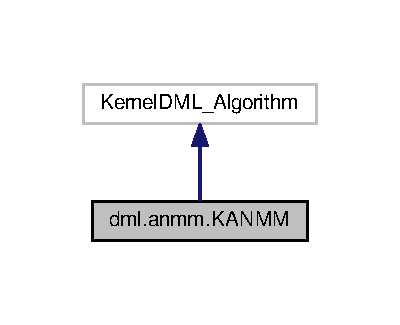
\includegraphics[width=192pt]{classdml_1_1anmm_1_1KANMM__inherit__graph}
\end{center}
\end{figure}


Collaboration diagram for dml.\+anmm.\+K\+A\+N\+MM\+:
\nopagebreak
\begin{figure}[H]
\begin{center}
\leavevmode
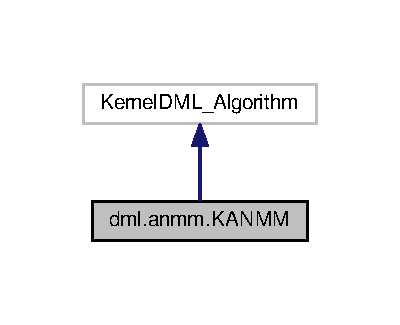
\includegraphics[width=192pt]{classdml_1_1anmm_1_1KANMM__coll__graph}
\end{center}
\end{figure}
\subsection*{Public Member Functions}
\begin{DoxyCompactItemize}
\item 
def {\bfseries \+\_\+\+\_\+init\+\_\+\+\_\+} (self, num\+\_\+dims=None, n\+\_\+friends=3, n\+\_\+enemies=1, kernel=\char`\"{}linear\char`\"{}, gamma=None, degree=3, coef0=1, kernel\+\_\+params=None)\hypertarget{classdml_1_1anmm_1_1KANMM_a27564180c8e609b664a9682ff062c494}{}\label{classdml_1_1anmm_1_1KANMM_a27564180c8e609b664a9682ff062c494}

\item 
def \hyperlink{classdml_1_1anmm_1_1KANMM_a48d48a25293d9816baccc3d5498b5558}{fit} (self, X, y)
\item 
def \hyperlink{classdml_1_1anmm_1_1KANMM_a20b5a78cf977077120a10bc0d8716ddf}{transformer} (self)
\end{DoxyCompactItemize}
\subsection*{Public Attributes}
\begin{DoxyCompactItemize}
\item 
{\bfseries num\+\_\+dims\+\_\+}\hypertarget{classdml_1_1anmm_1_1KANMM_a1466d59e8fd54aeecfc3d616d4925add}{}\label{classdml_1_1anmm_1_1KANMM_a1466d59e8fd54aeecfc3d616d4925add}

\item 
{\bfseries n\+\_\+fr\+\_\+}\hypertarget{classdml_1_1anmm_1_1KANMM_a1acb8cd44dbdb1b5718760d60e45ebb1}{}\label{classdml_1_1anmm_1_1KANMM_a1acb8cd44dbdb1b5718760d60e45ebb1}

\item 
{\bfseries n\+\_\+en\+\_\+}\hypertarget{classdml_1_1anmm_1_1KANMM_a0141f19aabfabe710a62984ca04d6ace}{}\label{classdml_1_1anmm_1_1KANMM_a0141f19aabfabe710a62984ca04d6ace}

\item 
{\bfseries kernel\+\_\+}\hypertarget{classdml_1_1anmm_1_1KANMM_a7c3574c66f8622eda7b2a9dc3ecb9745}{}\label{classdml_1_1anmm_1_1KANMM_a7c3574c66f8622eda7b2a9dc3ecb9745}

\item 
{\bfseries gamma\+\_\+}\hypertarget{classdml_1_1anmm_1_1KANMM_a3a23b318340983e513afb8379ba0ddd0}{}\label{classdml_1_1anmm_1_1KANMM_a3a23b318340983e513afb8379ba0ddd0}

\item 
{\bfseries degree\+\_\+}\hypertarget{classdml_1_1anmm_1_1KANMM_ae0f39a414f5eead101b9dffdd957a0e7}{}\label{classdml_1_1anmm_1_1KANMM_ae0f39a414f5eead101b9dffdd957a0e7}

\item 
{\bfseries coef0\+\_\+}\hypertarget{classdml_1_1anmm_1_1KANMM_a70084d43dec7c666074faa631e518a83}{}\label{classdml_1_1anmm_1_1KANMM_a70084d43dec7c666074faa631e518a83}

\item 
{\bfseries kernel\+\_\+params\+\_\+}\hypertarget{classdml_1_1anmm_1_1KANMM_a39d2ec090de06d21beba53c854d429fb}{}\label{classdml_1_1anmm_1_1KANMM_a39d2ec090de06d21beba53c854d429fb}

\item 
{\bfseries y\+\_\+}\hypertarget{classdml_1_1anmm_1_1KANMM_ae2913f61e8cb0b6823144f27d6d235b0}{}\label{classdml_1_1anmm_1_1KANMM_ae2913f61e8cb0b6823144f27d6d235b0}

\item 
{\bfseries distance\+\_\+matrix\+\_\+}\hypertarget{classdml_1_1anmm_1_1KANMM_a9a3de9d9f8ef278a11afb80aa94feea4}{}\label{classdml_1_1anmm_1_1KANMM_a9a3de9d9f8ef278a11afb80aa94feea4}

\item 
{\bfseries d\+\_\+}\hypertarget{classdml_1_1anmm_1_1KANMM_ad60072d5b0df220ef629878ff8bbf076}{}\label{classdml_1_1anmm_1_1KANMM_ad60072d5b0df220ef629878ff8bbf076}

\item 
{\bfseries eig\+\_\+vecs\+\_\+}\hypertarget{classdml_1_1anmm_1_1KANMM_a15baae5fb44f932523a5705f4313ad24}{}\label{classdml_1_1anmm_1_1KANMM_a15baae5fb44f932523a5705f4313ad24}

\item 
{\bfseries eig\+\_\+pairs\+\_\+}\hypertarget{classdml_1_1anmm_1_1KANMM_aff203f3ca66097f06d7c6bc4140d2cf4}{}\label{classdml_1_1anmm_1_1KANMM_aff203f3ca66097f06d7c6bc4140d2cf4}

\item 
{\bfseries L\+\_\+}\hypertarget{classdml_1_1anmm_1_1KANMM_a4d7e2a756480516b65c31309d70ff3e4}{}\label{classdml_1_1anmm_1_1KANMM_a4d7e2a756480516b65c31309d70ff3e4}

\end{DoxyCompactItemize}


\subsection{Detailed Description}
\begin{DoxyVerb}The kernelized version of ANMM.

Parameters
----------
num_dims : int, default=None
    Dimension desired for the transformed data.

n_friends : int, default=3
    Number of nearest same-class neighbors to compute homogeneus neighborhood.

n_enemies : int, default=1
    Number of nearest different-class neighbors to compute heterogeneus neigborhood.

kernel : "linear" | "poly" | "rbf" | "sigmoid" | "cosine" | "precomputed"
    Kernel. Default="linear".

gamma : float, default=1/n_features
    Kernel coefficient for rbf, poly and sigmoid kernels. Ignored by other
    kernels.

degree : int, default=3
    Degree for poly kernels. Ignored by other kernels.

coef0 : float, default=1
    Independent term in poly and sigmoid kernels.
    Ignored by other kernels.

kernel_params : mapping of string to any, default=None
    Parameters (keyword arguments) and values for kernel passed as
    callable object. Ignored by other kernels.


References
----------
    Fei Wang and Changshui Zhang. “Feature extraction by maximizing the average neighborhood
    margin”. In: Computer Vision and Pattern Recognition, 2007. CVPR’07. IEEE Conference on.
    IEEE. 2007, pages. 1-8.
\end{DoxyVerb}
 

\subsection{Member Function Documentation}
\index{dml\+::anmm\+::\+K\+A\+N\+MM@{dml\+::anmm\+::\+K\+A\+N\+MM}!fit@{fit}}
\index{fit@{fit}!dml\+::anmm\+::\+K\+A\+N\+MM@{dml\+::anmm\+::\+K\+A\+N\+MM}}
\subsubsection[{\texorpdfstring{fit(self, X, y)}{fit(self, X, y)}}]{\setlength{\rightskip}{0pt plus 5cm}def dml.\+anmm.\+K\+A\+N\+M\+M.\+fit (
\begin{DoxyParamCaption}
\item[{}]{self, }
\item[{}]{X, }
\item[{}]{y}
\end{DoxyParamCaption}
)}\hypertarget{classdml_1_1anmm_1_1KANMM_a48d48a25293d9816baccc3d5498b5558}{}\label{classdml_1_1anmm_1_1KANMM_a48d48a25293d9816baccc3d5498b5558}
\begin{DoxyVerb}Fit the model from the data in X and the labels in y.

Parameters
----------
X : array-like, shape (N x d)
    Training vector, where N is the number of samples, and d is the number of features.

y : array-like, shape (N)
    Labels vector, where N is the number of samples.

Returns
-------
self : object
    Returns the instance itself.
\end{DoxyVerb}
 \index{dml\+::anmm\+::\+K\+A\+N\+MM@{dml\+::anmm\+::\+K\+A\+N\+MM}!transformer@{transformer}}
\index{transformer@{transformer}!dml\+::anmm\+::\+K\+A\+N\+MM@{dml\+::anmm\+::\+K\+A\+N\+MM}}
\subsubsection[{\texorpdfstring{transformer(self)}{transformer(self)}}]{\setlength{\rightskip}{0pt plus 5cm}def dml.\+anmm.\+K\+A\+N\+M\+M.\+transformer (
\begin{DoxyParamCaption}
\item[{}]{self}
\end{DoxyParamCaption}
)}\hypertarget{classdml_1_1anmm_1_1KANMM_a20b5a78cf977077120a10bc0d8716ddf}{}\label{classdml_1_1anmm_1_1KANMM_a20b5a78cf977077120a10bc0d8716ddf}
\begin{DoxyVerb}Obtains the learned projection.

Returns
-------
A : (d'x N) matrix, where d' is the desired output dimension, and N is the number of samples.
    To apply A to a new sample x, A must be multiplied by the kernel vector of dimension N
    obtained by taking the kernels between x and each training sample.
\end{DoxyVerb}
 

The documentation for this class was generated from the following file\+:\begin{DoxyCompactItemize}
\item 
dml/anmm.\+pyx\end{DoxyCompactItemize}

\hypertarget{classdml_1_1kda_1_1KDA}{}\section{dml.\+kda.\+K\+DA Class Reference}
\label{classdml_1_1kda_1_1KDA}\index{dml.\+kda.\+K\+DA@{dml.\+kda.\+K\+DA}}


Inheritance diagram for dml.\+kda.\+K\+DA\+:
\nopagebreak
\begin{figure}[H]
\begin{center}
\leavevmode
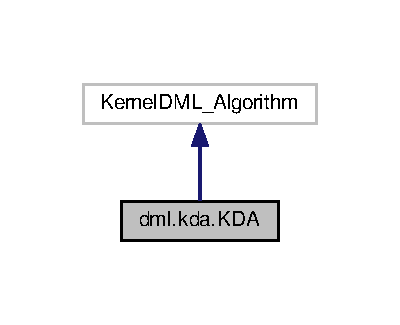
\includegraphics[width=192pt]{classdml_1_1kda_1_1KDA__inherit__graph}
\end{center}
\end{figure}


Collaboration diagram for dml.\+kda.\+K\+DA\+:
\nopagebreak
\begin{figure}[H]
\begin{center}
\leavevmode
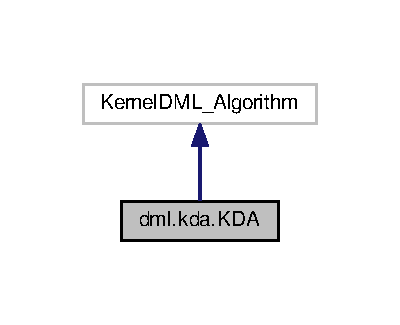
\includegraphics[width=192pt]{classdml_1_1kda_1_1KDA__coll__graph}
\end{center}
\end{figure}
\subsection*{Public Member Functions}
\begin{DoxyCompactItemize}
\item 
def {\bfseries \+\_\+\+\_\+init\+\_\+\+\_\+} (self, solver=\textquotesingle{}eigen\textquotesingle{}, n\+\_\+components=None, tol=1e-\/4, kernel=\char`\"{}linear\char`\"{}, gamma=\+None, degree=3, coef0=1, kernel\+\_\+params=\+None)\hypertarget{classdml_1_1kda_1_1KDA_a36fe718d7f2acf4664420bc1e370ada9}{}\label{classdml_1_1kda_1_1KDA_a36fe718d7f2acf4664420bc1e370ada9}

\item 
def \hyperlink{classdml_1_1kda_1_1KDA_aecc0bd189d2080ac3cb2248e3ded47c4}{transformer} (self)
\item 
def \hyperlink{classdml_1_1kda_1_1KDA_a1a22e6ac1e9833d1a6cca60c9bc832d8}{fit} (self, X, y)
\end{DoxyCompactItemize}
\subsection*{Public Attributes}
\begin{DoxyCompactItemize}
\item 
{\bfseries solver\+\_\+}\hypertarget{classdml_1_1kda_1_1KDA_ac314973f2e20b7aa4ed1fcbc9f6d80da}{}\label{classdml_1_1kda_1_1KDA_ac314973f2e20b7aa4ed1fcbc9f6d80da}

\item 
{\bfseries n\+\_\+components\+\_\+}\hypertarget{classdml_1_1kda_1_1KDA_a45f464ac054517ab88af2b82f58a75fe}{}\label{classdml_1_1kda_1_1KDA_a45f464ac054517ab88af2b82f58a75fe}

\item 
{\bfseries tol\+\_\+}\hypertarget{classdml_1_1kda_1_1KDA_afda7891fef268f00e5c767afde511aa8}{}\label{classdml_1_1kda_1_1KDA_afda7891fef268f00e5c767afde511aa8}

\item 
{\bfseries kernel\+\_\+}\hypertarget{classdml_1_1kda_1_1KDA_a79cdebd296f9389db1eebf4fd8831322}{}\label{classdml_1_1kda_1_1KDA_a79cdebd296f9389db1eebf4fd8831322}

\item 
{\bfseries gamma\+\_\+}\hypertarget{classdml_1_1kda_1_1KDA_aabe1af31aefce2cc04742a84640a14c2}{}\label{classdml_1_1kda_1_1KDA_aabe1af31aefce2cc04742a84640a14c2}

\item 
{\bfseries degree\+\_\+}\hypertarget{classdml_1_1kda_1_1KDA_aad0e6e4c05920afc27548c732a76655d}{}\label{classdml_1_1kda_1_1KDA_aad0e6e4c05920afc27548c732a76655d}

\item 
{\bfseries coef0\+\_\+}\hypertarget{classdml_1_1kda_1_1KDA_ad86ca60accb840611b2db09140b5d671}{}\label{classdml_1_1kda_1_1KDA_ad86ca60accb840611b2db09140b5d671}

\item 
{\bfseries kernel\+\_\+params\+\_\+}\hypertarget{classdml_1_1kda_1_1KDA_ad2d07b7dee9cdea07ad1dc0c6bc7fcd5}{}\label{classdml_1_1kda_1_1KDA_ad2d07b7dee9cdea07ad1dc0c6bc7fcd5}

\item 
{\bfseries y\+\_\+}\hypertarget{classdml_1_1kda_1_1KDA_a7004928097d9a4eebe9b2979ac563beb}{}\label{classdml_1_1kda_1_1KDA_a7004928097d9a4eebe9b2979ac563beb}

\item 
{\bfseries L\+\_\+}\hypertarget{classdml_1_1kda_1_1KDA_a8a56310c6b6918a52af4a7260e780fdd}{}\label{classdml_1_1kda_1_1KDA_a8a56310c6b6918a52af4a7260e780fdd}

\end{DoxyCompactItemize}


\subsection{Detailed Description}
\begin{DoxyVerb}Kernel Discriminant Analysis (KDA)

Discriminant Analysis in high dimensionality using the kernel trick.

Parameters
----------

solver : string, default='eigen'.

    Solver to use, posible values:
        - 'eigen': Eigenvalue decomposition.

n_components : int, default=None.

    Number of components (lower than number of classes -1) for dimensionality reduction.

tol : float, default=1e-4

    Singularity toleration level.

kernel : "linear" | "poly" | "rbf" | "sigmoid" | "cosine" | "precomputed"
    Kernel. Default="linear".

gamma : float, default=1/n_features
    Kernel coefficient for rbf, poly and sigmoid kernels. Ignored by other
    kernels.

degree : int, default=3
    Degree for poly kernels. Ignored by other kernels.

coef0 : float, default=1
    Independent term in poly and sigmoid kernels.
    Ignored by other kernels.

kernel_params : mapping of string to any, default=None
    Parameters (keyword arguments) and values for kernel passed as
    callable object. Ignored by other kernels.

References
----------
    Sebastian Mika et al. “Fisher discriminant analysis with kernels”. In: Neural networks for signal
    processing IX, 1999. Proceedings of the 1999 IEEE signal processing society workshop. Ieee. 1999,
    pages 41-48.\end{DoxyVerb}
 

\subsection{Member Function Documentation}
\index{dml\+::kda\+::\+K\+DA@{dml\+::kda\+::\+K\+DA}!fit@{fit}}
\index{fit@{fit}!dml\+::kda\+::\+K\+DA@{dml\+::kda\+::\+K\+DA}}
\subsubsection[{\texorpdfstring{fit(self, X, y)}{fit(self, X, y)}}]{\setlength{\rightskip}{0pt plus 5cm}def dml.\+kda.\+K\+D\+A.\+fit (
\begin{DoxyParamCaption}
\item[{}]{self, }
\item[{}]{X, }
\item[{}]{y}
\end{DoxyParamCaption}
)}\hypertarget{classdml_1_1kda_1_1KDA_a1a22e6ac1e9833d1a6cca60c9bc832d8}{}\label{classdml_1_1kda_1_1KDA_a1a22e6ac1e9833d1a6cca60c9bc832d8}
\begin{DoxyVerb}Fit the model from the data in X and the labels in y.

Parameters
----------
X : array-like, shape (N x d)
    Training vector, where N is the number of samples, and d is the number of features.

y : array-like, shape (N)
    Labels vector, where N is the number of samples.

Returns
-------
self : object
    Returns the instance itself.
\end{DoxyVerb}
 \index{dml\+::kda\+::\+K\+DA@{dml\+::kda\+::\+K\+DA}!transformer@{transformer}}
\index{transformer@{transformer}!dml\+::kda\+::\+K\+DA@{dml\+::kda\+::\+K\+DA}}
\subsubsection[{\texorpdfstring{transformer(self)}{transformer(self)}}]{\setlength{\rightskip}{0pt plus 5cm}def dml.\+kda.\+K\+D\+A.\+transformer (
\begin{DoxyParamCaption}
\item[{}]{self}
\end{DoxyParamCaption}
)}\hypertarget{classdml_1_1kda_1_1KDA_aecc0bd189d2080ac3cb2248e3ded47c4}{}\label{classdml_1_1kda_1_1KDA_aecc0bd189d2080ac3cb2248e3ded47c4}
\begin{DoxyVerb}Obtains the learned projection.

Returns
-------
A : (d'x N) matrix, where d' is the desired output dimension, and N is the number of samples.
    To apply A to a new sample x, A must be multiplied by the kernel vector of dimension N
    obtained by taking the kernels between x and each training sample.
\end{DoxyVerb}
 

The documentation for this class was generated from the following file\+:\begin{DoxyCompactItemize}
\item 
dml/kda.\+pyx\end{DoxyCompactItemize}

\hypertarget{classdml_1_1dmlmj_1_1KDMLMJ}{}\section{dml.\+dmlmj.\+K\+D\+M\+L\+MJ Class Reference}
\label{classdml_1_1dmlmj_1_1KDMLMJ}\index{dml.\+dmlmj.\+K\+D\+M\+L\+MJ@{dml.\+dmlmj.\+K\+D\+M\+L\+MJ}}


Inheritance diagram for dml.\+dmlmj.\+K\+D\+M\+L\+MJ\+:
\nopagebreak
\begin{figure}[H]
\begin{center}
\leavevmode
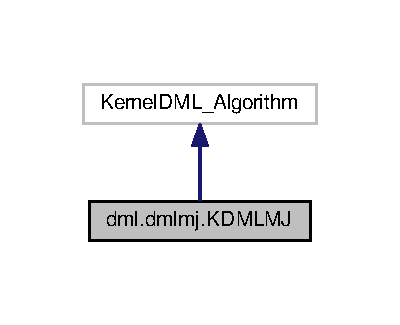
\includegraphics[width=192pt]{classdml_1_1dmlmj_1_1KDMLMJ__inherit__graph}
\end{center}
\end{figure}


Collaboration diagram for dml.\+dmlmj.\+K\+D\+M\+L\+MJ\+:
\nopagebreak
\begin{figure}[H]
\begin{center}
\leavevmode
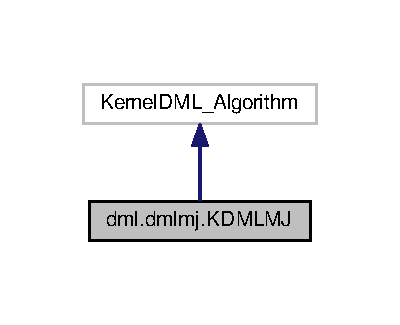
\includegraphics[width=192pt]{classdml_1_1dmlmj_1_1KDMLMJ__coll__graph}
\end{center}
\end{figure}
\subsection*{Public Member Functions}
\begin{DoxyCompactItemize}
\item 
def {\bfseries \+\_\+\+\_\+init\+\_\+\+\_\+} (self, num\+\_\+dims=None, n\+\_\+neighbors=3, alpha=0.\+001, reg\+\_\+tol=1e-\/10, kernel=\char`\"{}linear\char`\"{}, gamma=\+None, degree=3, coef0=1, kernel\+\_\+params=\+None)\hypertarget{classdml_1_1dmlmj_1_1KDMLMJ_ac8acdf1d02e47508c9c879fa2a7c99ff}{}\label{classdml_1_1dmlmj_1_1KDMLMJ_ac8acdf1d02e47508c9c879fa2a7c99ff}

\item 
def \hyperlink{classdml_1_1dmlmj_1_1KDMLMJ_a18a53c1278081748f9d381deebfbef38}{transformer} (self)
\item 
def \hyperlink{classdml_1_1dmlmj_1_1KDMLMJ_ae88dd077200a6327abb4d1f45855eb66}{metadata} (self)
\item 
def \hyperlink{classdml_1_1dmlmj_1_1KDMLMJ_a6411e45a04c4af41c246f578fc80d539}{fit} (self, X, y)
\end{DoxyCompactItemize}
\subsection*{Public Attributes}
\begin{DoxyCompactItemize}
\item 
{\bfseries num\+\_\+dims\+\_\+}\hypertarget{classdml_1_1dmlmj_1_1KDMLMJ_a000981c8ffb25f30e8b9892426b82cfd}{}\label{classdml_1_1dmlmj_1_1KDMLMJ_a000981c8ffb25f30e8b9892426b82cfd}

\item 
{\bfseries k\+\_\+}\hypertarget{classdml_1_1dmlmj_1_1KDMLMJ_a8b980a2329a826e0fae6721307d4e4cf}{}\label{classdml_1_1dmlmj_1_1KDMLMJ_a8b980a2329a826e0fae6721307d4e4cf}

\item 
{\bfseries alpha\+\_\+}\hypertarget{classdml_1_1dmlmj_1_1KDMLMJ_aefc7696b195cd5f72cbb721f477e66f1}{}\label{classdml_1_1dmlmj_1_1KDMLMJ_aefc7696b195cd5f72cbb721f477e66f1}

\item 
{\bfseries reg\+\_\+tol\+\_\+}\hypertarget{classdml_1_1dmlmj_1_1KDMLMJ_a5d895da19ab728354715d7b517f224a6}{}\label{classdml_1_1dmlmj_1_1KDMLMJ_a5d895da19ab728354715d7b517f224a6}

\item 
{\bfseries kernel\+\_\+}\hypertarget{classdml_1_1dmlmj_1_1KDMLMJ_a3f3bab232d0bfe22a2e94d6d3a1d5a33}{}\label{classdml_1_1dmlmj_1_1KDMLMJ_a3f3bab232d0bfe22a2e94d6d3a1d5a33}

\item 
{\bfseries gamma\+\_\+}\hypertarget{classdml_1_1dmlmj_1_1KDMLMJ_a971b7c76f5df2c8320b24ef242b765f2}{}\label{classdml_1_1dmlmj_1_1KDMLMJ_a971b7c76f5df2c8320b24ef242b765f2}

\item 
{\bfseries degree\+\_\+}\hypertarget{classdml_1_1dmlmj_1_1KDMLMJ_a235139ddfa7855dda240ca7d61b7b021}{}\label{classdml_1_1dmlmj_1_1KDMLMJ_a235139ddfa7855dda240ca7d61b7b021}

\item 
{\bfseries coef0\+\_\+}\hypertarget{classdml_1_1dmlmj_1_1KDMLMJ_af30e7f2b40fca77f1e505b1d12cec80d}{}\label{classdml_1_1dmlmj_1_1KDMLMJ_af30e7f2b40fca77f1e505b1d12cec80d}

\item 
{\bfseries kernel\+\_\+params\+\_\+}\hypertarget{classdml_1_1dmlmj_1_1KDMLMJ_afea69888606c40c366c0d919fd030a4e}{}\label{classdml_1_1dmlmj_1_1KDMLMJ_afea69888606c40c366c0d919fd030a4e}

\item 
{\bfseries acum\+\_\+eig\+\_\+}\hypertarget{classdml_1_1dmlmj_1_1KDMLMJ_ad63c0b501ee0f6f892fadbb08e865a6f}{}\label{classdml_1_1dmlmj_1_1KDMLMJ_ad63c0b501ee0f6f892fadbb08e865a6f}

\item 
{\bfseries nd\+\_\+}\hypertarget{classdml_1_1dmlmj_1_1KDMLMJ_a3c51fc6cce7dd08bd1ee2b0846e4620a}{}\label{classdml_1_1dmlmj_1_1KDMLMJ_a3c51fc6cce7dd08bd1ee2b0846e4620a}

\item 
{\bfseries y\+\_\+}\hypertarget{classdml_1_1dmlmj_1_1KDMLMJ_aecdd67ff2d44aae35b8552b797c78ca6}{}\label{classdml_1_1dmlmj_1_1KDMLMJ_aecdd67ff2d44aae35b8552b797c78ca6}

\item 
{\bfseries d\+\_\+}\hypertarget{classdml_1_1dmlmj_1_1KDMLMJ_a1e76efa422a8148224ccd09b6c3d6f4e}{}\label{classdml_1_1dmlmj_1_1KDMLMJ_a1e76efa422a8148224ccd09b6c3d6f4e}

\item 
{\bfseries eig\+\_\+vecs\+\_\+}\hypertarget{classdml_1_1dmlmj_1_1KDMLMJ_abb7bfed9c73bff7fb186b01356e3b9bd}{}\label{classdml_1_1dmlmj_1_1KDMLMJ_abb7bfed9c73bff7fb186b01356e3b9bd}

\item 
{\bfseries eig\+\_\+pairs\+\_\+}\hypertarget{classdml_1_1dmlmj_1_1KDMLMJ_aef04278df7cf9c52234da8e3b2037e23}{}\label{classdml_1_1dmlmj_1_1KDMLMJ_aef04278df7cf9c52234da8e3b2037e23}

\item 
{\bfseries L\+\_\+}\hypertarget{classdml_1_1dmlmj_1_1KDMLMJ_ad635b9074df3023e1b24b2968ffab2ec}{}\label{classdml_1_1dmlmj_1_1KDMLMJ_ad635b9074df3023e1b24b2968ffab2ec}

\item 
{\bfseries acum\+\_\+eigvals\+\_\+}\hypertarget{classdml_1_1dmlmj_1_1KDMLMJ_a04f8492dad9b259c59b76c486456cc96}{}\label{classdml_1_1dmlmj_1_1KDMLMJ_a04f8492dad9b259c59b76c486456cc96}

\end{DoxyCompactItemize}


\subsection{Detailed Description}
\begin{DoxyVerb}The kernelized version of DMLMJ.

Parameters
----------
num_dims : int, default=None
    Dimension desired for the transformed data.

n_neighbors : int, default=3
    Number of neighbors to consider in the computation of the difference spaces.

alpha : float, default=0.001
    Regularization parameter for inverse matrix computation.

reg_tol : float, default=1e-10
    Tolerance threshold for applying regularization. The tolerance is compared with the matrix determinant.

kernel : "linear" | "poly" | "rbf" | "sigmoid" | "cosine" | "precomputed"
    Kernel. Default="linear".

gamma : float, default=1/n_features
    Kernel coefficient for rbf, poly and sigmoid kernels. Ignored by other
    kernels.

degree : int, default=3
    Degree for poly kernels. Ignored by other kernels.

coef0 : float, default=1
    Independent term in poly and sigmoid kernels.
    Ignored by other kernels.

kernel_params : mapping of string to any, default=None
    Parameters (keyword arguments) and values for kernel passed as
    callable object. Ignored by other kernels.

References
----------
    Bac Nguyen, Carlos Morell and Bernard De Baets. “Supervised distance metric learning through
    maximization of the Jeffrey divergence”. In: Pattern Recognition 64 (2017), pages 215-225.
\end{DoxyVerb}
 

\subsection{Member Function Documentation}
\index{dml\+::dmlmj\+::\+K\+D\+M\+L\+MJ@{dml\+::dmlmj\+::\+K\+D\+M\+L\+MJ}!fit@{fit}}
\index{fit@{fit}!dml\+::dmlmj\+::\+K\+D\+M\+L\+MJ@{dml\+::dmlmj\+::\+K\+D\+M\+L\+MJ}}
\subsubsection[{\texorpdfstring{fit(self, X, y)}{fit(self, X, y)}}]{\setlength{\rightskip}{0pt plus 5cm}def dml.\+dmlmj.\+K\+D\+M\+L\+M\+J.\+fit (
\begin{DoxyParamCaption}
\item[{}]{self, }
\item[{}]{X, }
\item[{}]{y}
\end{DoxyParamCaption}
)}\hypertarget{classdml_1_1dmlmj_1_1KDMLMJ_a6411e45a04c4af41c246f578fc80d539}{}\label{classdml_1_1dmlmj_1_1KDMLMJ_a6411e45a04c4af41c246f578fc80d539}
\begin{DoxyVerb}Fit the model from the data in X and the labels in y.

Parameters
----------
X : array-like, shape (N x d)
    Training vector, where N is the number of samples, and d is the number of features.

y : array-like, shape (N)
    Labels vector, where N is the number of samples.

Returns
-------
self : object
    Returns the instance itself.
\end{DoxyVerb}
 \index{dml\+::dmlmj\+::\+K\+D\+M\+L\+MJ@{dml\+::dmlmj\+::\+K\+D\+M\+L\+MJ}!metadata@{metadata}}
\index{metadata@{metadata}!dml\+::dmlmj\+::\+K\+D\+M\+L\+MJ@{dml\+::dmlmj\+::\+K\+D\+M\+L\+MJ}}
\subsubsection[{\texorpdfstring{metadata(self)}{metadata(self)}}]{\setlength{\rightskip}{0pt plus 5cm}def dml.\+dmlmj.\+K\+D\+M\+L\+M\+J.\+metadata (
\begin{DoxyParamCaption}
\item[{}]{self}
\end{DoxyParamCaption}
)}\hypertarget{classdml_1_1dmlmj_1_1KDMLMJ_ae88dd077200a6327abb4d1f45855eb66}{}\label{classdml_1_1dmlmj_1_1KDMLMJ_ae88dd077200a6327abb4d1f45855eb66}
\begin{DoxyVerb}Obtains algorithm metadata.

Returns
-------
meta : A dictionary with the following metadata:
    acum_eig : eigenvalue rate accumulated in the learned output respect to the total dimension.

    num_dims : dimension of the reduced data.
\end{DoxyVerb}
 \index{dml\+::dmlmj\+::\+K\+D\+M\+L\+MJ@{dml\+::dmlmj\+::\+K\+D\+M\+L\+MJ}!transformer@{transformer}}
\index{transformer@{transformer}!dml\+::dmlmj\+::\+K\+D\+M\+L\+MJ@{dml\+::dmlmj\+::\+K\+D\+M\+L\+MJ}}
\subsubsection[{\texorpdfstring{transformer(self)}{transformer(self)}}]{\setlength{\rightskip}{0pt plus 5cm}def dml.\+dmlmj.\+K\+D\+M\+L\+M\+J.\+transformer (
\begin{DoxyParamCaption}
\item[{}]{self}
\end{DoxyParamCaption}
)}\hypertarget{classdml_1_1dmlmj_1_1KDMLMJ_a18a53c1278081748f9d381deebfbef38}{}\label{classdml_1_1dmlmj_1_1KDMLMJ_a18a53c1278081748f9d381deebfbef38}
\begin{DoxyVerb}Obtains the learned projection.

Returns
-------
A : (d'x N) matrix, where d' is the desired output dimension, and N is the number of samples.
    To apply A to a new sample x, A must be multiplied by the kernel vector of dimension N
    obtained by taking the kernels between x and each training sample.
\end{DoxyVerb}
 

The documentation for this class was generated from the following file\+:\begin{DoxyCompactItemize}
\item 
dml/dmlmj.\+pyx\end{DoxyCompactItemize}

\hypertarget{classdml_1_1dml__algorithm_1_1KernelDML__Algorithm}{}\section{dml.\+dml\+\_\+algorithm.\+Kernel\+D\+M\+L\+\_\+\+Algorithm Class Reference}
\label{classdml_1_1dml__algorithm_1_1KernelDML__Algorithm}\index{dml.\+dml\+\_\+algorithm.\+Kernel\+D\+M\+L\+\_\+\+Algorithm@{dml.\+dml\+\_\+algorithm.\+Kernel\+D\+M\+L\+\_\+\+Algorithm}}


Inheritance diagram for dml.\+dml\+\_\+algorithm.\+Kernel\+D\+M\+L\+\_\+\+Algorithm\+:\nopagebreak
\begin{figure}[H]
\begin{center}
\leavevmode
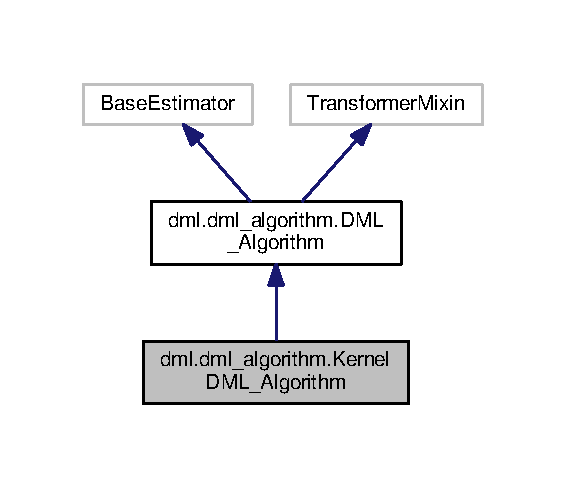
\includegraphics[width=272pt]{classdml_1_1dml__algorithm_1_1KernelDML__Algorithm__inherit__graph}
\end{center}
\end{figure}


Collaboration diagram for dml.\+dml\+\_\+algorithm.\+Kernel\+D\+M\+L\+\_\+\+Algorithm\+:\nopagebreak
\begin{figure}[H]
\begin{center}
\leavevmode
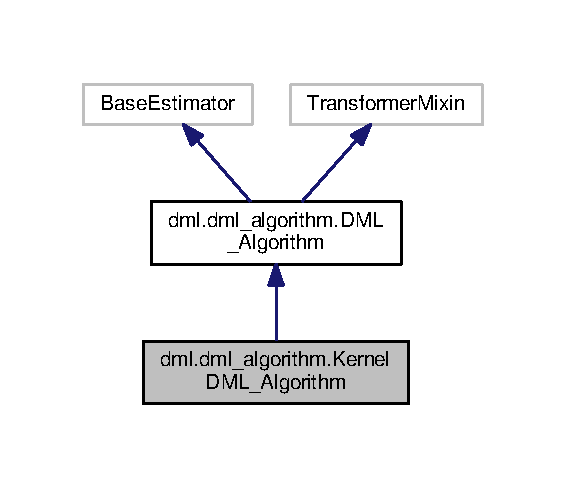
\includegraphics[width=272pt]{classdml_1_1dml__algorithm_1_1KernelDML__Algorithm__coll__graph}
\end{center}
\end{figure}
\subsection*{Public Member Functions}
\begin{DoxyCompactItemize}
\item 
def {\bfseries \+\_\+\+\_\+init\+\_\+\+\_\+} (self)\hypertarget{classdml_1_1dml__algorithm_1_1KernelDML__Algorithm_ac18f6c2e3cde917c89349b719461dc68}{}\label{classdml_1_1dml__algorithm_1_1KernelDML__Algorithm_ac18f6c2e3cde917c89349b719461dc68}

\item 
def \hyperlink{classdml_1_1dml__algorithm_1_1KernelDML__Algorithm_af2875484bd1522bf0db61d6507ee67a2}{transform} (self, X=None)
\end{DoxyCompactItemize}
\subsection*{Public Attributes}
\begin{DoxyCompactItemize}
\item 
{\bfseries kernel\+\_\+}\hypertarget{classdml_1_1dml__algorithm_1_1KernelDML__Algorithm_a28fbb59e6b3a75ee25f06dc432700124}{}\label{classdml_1_1dml__algorithm_1_1KernelDML__Algorithm_a28fbb59e6b3a75ee25f06dc432700124}

\end{DoxyCompactItemize}


\subsection{Detailed Description}
\begin{DoxyVerb}    Abstract class that defines a kernel distance metric learning algorithm.
    Distance metric learning are implemented as subclasses of KernelDML_Algorithm.
    A Kernel DML Algorithm can compute a (d' x n) transformer that maps the high dimensional data using the kernel trick.
    Kernel DML subclasses must override the transformer method, providing the matrix A that performs the kernel trick, that is
    ..math:: Lx = A(K(x_1,x),\\dots,K(x_n,x)),
    where L is the high dimensional transformer and K is the kernel function.
\end{DoxyVerb}
 

\subsection{Member Function Documentation}
\index{dml\+::dml\+\_\+algorithm\+::\+Kernel\+D\+M\+L\+\_\+\+Algorithm@{dml\+::dml\+\_\+algorithm\+::\+Kernel\+D\+M\+L\+\_\+\+Algorithm}!transform@{transform}}
\index{transform@{transform}!dml\+::dml\+\_\+algorithm\+::\+Kernel\+D\+M\+L\+\_\+\+Algorithm@{dml\+::dml\+\_\+algorithm\+::\+Kernel\+D\+M\+L\+\_\+\+Algorithm}}
\subsubsection[{\texorpdfstring{transform(self, X=\+None)}{transform(self, X=None)}}]{\setlength{\rightskip}{0pt plus 5cm}def dml.\+dml\+\_\+algorithm.\+Kernel\+D\+M\+L\+\_\+\+Algorithm.\+transform (
\begin{DoxyParamCaption}
\item[{}]{self, }
\item[{}]{X = {\ttfamily None}}
\end{DoxyParamCaption}
)}\hypertarget{classdml_1_1dml__algorithm_1_1KernelDML__Algorithm_af2875484bd1522bf0db61d6507ee67a2}{}\label{classdml_1_1dml__algorithm_1_1KernelDML__Algorithm_af2875484bd1522bf0db61d6507ee67a2}
\begin{DoxyVerb}Applies the kernel transformation.

Parameters
----------
X : (N x d) matrix, optional
    Data to transform. If not supplied, the training data will be used.

Returns
-------
transformed: (N x d') matrix.
    Input data transformed by the learned mapping.
\end{DoxyVerb}
 

The documentation for this class was generated from the following file\+:\begin{DoxyCompactItemize}
\item 
dml/dml\+\_\+algorithm.\+py\end{DoxyCompactItemize}

\hypertarget{classdml_1_1lmnn_1_1KLMNN}{}\section{dml.\+lmnn.\+K\+L\+M\+NN Class Reference}
\label{classdml_1_1lmnn_1_1KLMNN}\index{dml.\+lmnn.\+K\+L\+M\+NN@{dml.\+lmnn.\+K\+L\+M\+NN}}


Inheritance diagram for dml.\+lmnn.\+K\+L\+M\+NN\+:
\nopagebreak
\begin{figure}[H]
\begin{center}
\leavevmode
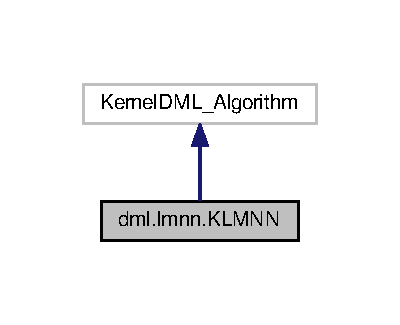
\includegraphics[width=192pt]{classdml_1_1lmnn_1_1KLMNN__inherit__graph}
\end{center}
\end{figure}


Collaboration diagram for dml.\+lmnn.\+K\+L\+M\+NN\+:
\nopagebreak
\begin{figure}[H]
\begin{center}
\leavevmode
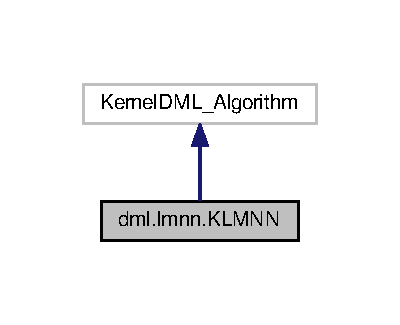
\includegraphics[width=192pt]{classdml_1_1lmnn_1_1KLMNN__coll__graph}
\end{center}
\end{figure}
\subsection*{Public Member Functions}
\begin{DoxyCompactItemize}
\item 
def {\bfseries \+\_\+\+\_\+init\+\_\+\+\_\+} (self, num\+\_\+dims=None, learning\+\_\+rate=\char`\"{}adaptive\char`\"{}, eta0=0.\+3, initial\+\_\+metric=None, max\+\_\+iter=100, prec=1e-\/8, tol=1e-\/8, k=3, mu=0.\+5, learn\+\_\+inc=1.\+01, learn\+\_\+dec=0.\+5, eta\+\_\+thres=1e-\/14, kernel=\char`\"{}linear\char`\"{}, gamma=\+None, degree=3, coef0=1, kernel\+\_\+params=\+None, target\+\_\+selection=\char`\"{}kernel\char`\"{})\hypertarget{classdml_1_1lmnn_1_1KLMNN_a339202f51571616cccbb7e82a9538277}{}\label{classdml_1_1lmnn_1_1KLMNN_a339202f51571616cccbb7e82a9538277}

\item 
def \hyperlink{classdml_1_1lmnn_1_1KLMNN_a77fd2cabceaea0fb542887add9dbeac0}{transformer} (self)
\item 
def \hyperlink{classdml_1_1lmnn_1_1KLMNN_aeb84c2956168954dbfddec72a01bc5dd}{metadata} (self)
\item 
def \hyperlink{classdml_1_1lmnn_1_1KLMNN_aed2b8b1e6de22d4e6170d4a270d78623}{fit} (self, X, y)
\end{DoxyCompactItemize}
\subsection*{Public Attributes}
\begin{DoxyCompactItemize}
\item 
{\bfseries num\+\_\+dims\+\_\+}\hypertarget{classdml_1_1lmnn_1_1KLMNN_abb851de27ec3faff37051a238f394643}{}\label{classdml_1_1lmnn_1_1KLMNN_abb851de27ec3faff37051a238f394643}

\item 
{\bfseries M0\+\_\+}\hypertarget{classdml_1_1lmnn_1_1KLMNN_ac4aed1cb11a11a2570f5a4079014145b}{}\label{classdml_1_1lmnn_1_1KLMNN_ac4aed1cb11a11a2570f5a4079014145b}

\item 
{\bfseries max\+\_\+it\+\_\+}\hypertarget{classdml_1_1lmnn_1_1KLMNN_a961924ae72463b2a081067479cc30874}{}\label{classdml_1_1lmnn_1_1KLMNN_a961924ae72463b2a081067479cc30874}

\item 
{\bfseries eta0\+\_\+}\hypertarget{classdml_1_1lmnn_1_1KLMNN_a8fc7f13d4728fbf2d59a29628d9fd541}{}\label{classdml_1_1lmnn_1_1KLMNN_a8fc7f13d4728fbf2d59a29628d9fd541}

\item 
{\bfseries eta\+\_\+}\hypertarget{classdml_1_1lmnn_1_1KLMNN_a29432e1998af99476b418dd3306e19d2}{}\label{classdml_1_1lmnn_1_1KLMNN_a29432e1998af99476b418dd3306e19d2}

\item 
{\bfseries learning\+\_\+}\hypertarget{classdml_1_1lmnn_1_1KLMNN_ab36d0340d3db07c79ad5ce558de81e6d}{}\label{classdml_1_1lmnn_1_1KLMNN_ab36d0340d3db07c79ad5ce558de81e6d}

\item 
{\bfseries adaptive\+\_\+}\hypertarget{classdml_1_1lmnn_1_1KLMNN_a9b1766d62f27a9fcf1dd08955eea24a2}{}\label{classdml_1_1lmnn_1_1KLMNN_a9b1766d62f27a9fcf1dd08955eea24a2}

\item 
{\bfseries eps\+\_\+}\hypertarget{classdml_1_1lmnn_1_1KLMNN_a8690102a13c5833ff12975e566ac009e}{}\label{classdml_1_1lmnn_1_1KLMNN_a8690102a13c5833ff12975e566ac009e}

\item 
{\bfseries tol\+\_\+}\hypertarget{classdml_1_1lmnn_1_1KLMNN_ac4b57f8045030eec291099398fde02d0}{}\label{classdml_1_1lmnn_1_1KLMNN_ac4b57f8045030eec291099398fde02d0}

\item 
{\bfseries mu\+\_\+}\hypertarget{classdml_1_1lmnn_1_1KLMNN_ae6bcf5f3ad2428e949671b07cbec638f}{}\label{classdml_1_1lmnn_1_1KLMNN_ae6bcf5f3ad2428e949671b07cbec638f}

\item 
{\bfseries k\+\_\+}\hypertarget{classdml_1_1lmnn_1_1KLMNN_ae08243645a6f30a97eaa150b45a2d0d3}{}\label{classdml_1_1lmnn_1_1KLMNN_ae08243645a6f30a97eaa150b45a2d0d3}

\item 
{\bfseries l\+\_\+inc\+\_\+}\hypertarget{classdml_1_1lmnn_1_1KLMNN_a967624698fe38a0088950d28db6febc9}{}\label{classdml_1_1lmnn_1_1KLMNN_a967624698fe38a0088950d28db6febc9}

\item 
{\bfseries l\+\_\+dec\+\_\+}\hypertarget{classdml_1_1lmnn_1_1KLMNN_ab4ed062fa5d6b209a1c77dce08a09e0a}{}\label{classdml_1_1lmnn_1_1KLMNN_ab4ed062fa5d6b209a1c77dce08a09e0a}

\item 
{\bfseries etamin\+\_\+}\hypertarget{classdml_1_1lmnn_1_1KLMNN_a977173f0328b2a58321e821c9d41b291}{}\label{classdml_1_1lmnn_1_1KLMNN_a977173f0328b2a58321e821c9d41b291}

\item 
{\bfseries target\+\_\+selection\+\_\+}\hypertarget{classdml_1_1lmnn_1_1KLMNN_aff31653d53a27d82e71d424cd93f404d}{}\label{classdml_1_1lmnn_1_1KLMNN_aff31653d53a27d82e71d424cd93f404d}

\item 
{\bfseries kernel\+\_\+}\hypertarget{classdml_1_1lmnn_1_1KLMNN_a3146f3cf23dd6a51717f45122e9fda22}{}\label{classdml_1_1lmnn_1_1KLMNN_a3146f3cf23dd6a51717f45122e9fda22}

\item 
{\bfseries gamma\+\_\+}\hypertarget{classdml_1_1lmnn_1_1KLMNN_abc910753eb9d73a87723794717442af0}{}\label{classdml_1_1lmnn_1_1KLMNN_abc910753eb9d73a87723794717442af0}

\item 
{\bfseries degree\+\_\+}\hypertarget{classdml_1_1lmnn_1_1KLMNN_ae5913646ad15aa139f56c4b8ed664e49}{}\label{classdml_1_1lmnn_1_1KLMNN_ae5913646ad15aa139f56c4b8ed664e49}

\item 
{\bfseries coef0\+\_\+}\hypertarget{classdml_1_1lmnn_1_1KLMNN_a0d2e3c2fd07d4e5461ff4539f4010aa2}{}\label{classdml_1_1lmnn_1_1KLMNN_a0d2e3c2fd07d4e5461ff4539f4010aa2}

\item 
{\bfseries kernel\+\_\+params\+\_\+}\hypertarget{classdml_1_1lmnn_1_1KLMNN_ac4645004c02107578699d63837bc1e33}{}\label{classdml_1_1lmnn_1_1KLMNN_ac4645004c02107578699d63837bc1e33}

\item 
{\bfseries num\+\_\+its\+\_\+}\hypertarget{classdml_1_1lmnn_1_1KLMNN_a3e2148e093e6b53110904c598a6d01cf}{}\label{classdml_1_1lmnn_1_1KLMNN_a3e2148e093e6b53110904c598a6d01cf}

\item 
{\bfseries initial\+\_\+error\+\_\+}\hypertarget{classdml_1_1lmnn_1_1KLMNN_afe372e1a7bd5c6f011fd5b7e3a4c9c3f}{}\label{classdml_1_1lmnn_1_1KLMNN_afe372e1a7bd5c6f011fd5b7e3a4c9c3f}

\item 
{\bfseries final\+\_\+error\+\_\+}\hypertarget{classdml_1_1lmnn_1_1KLMNN_a96e24c68a6c15bb57ef4aff80a74be9b}{}\label{classdml_1_1lmnn_1_1KLMNN_a96e24c68a6c15bb57ef4aff80a74be9b}

\item 
{\bfseries d\+\_\+}\hypertarget{classdml_1_1lmnn_1_1KLMNN_a06aff9be6116a21617b5887961b7cd95}{}\label{classdml_1_1lmnn_1_1KLMNN_a06aff9be6116a21617b5887961b7cd95}

\item 
{\bfseries nd\+\_\+}\hypertarget{classdml_1_1lmnn_1_1KLMNN_a8d387f7a0308e26a4b4f813d892327dd}{}\label{classdml_1_1lmnn_1_1KLMNN_a8d387f7a0308e26a4b4f813d892327dd}

\item 
{\bfseries L\+\_\+}\hypertarget{classdml_1_1lmnn_1_1KLMNN_ac43a8d7ba9a1c15dfe40de49e2293a84}{}\label{classdml_1_1lmnn_1_1KLMNN_ac43a8d7ba9a1c15dfe40de49e2293a84}

\item 
{\bfseries X\+\_\+}\hypertarget{classdml_1_1lmnn_1_1KLMNN_a9e090d67748917ad69b44dfcd3d49109}{}\label{classdml_1_1lmnn_1_1KLMNN_a9e090d67748917ad69b44dfcd3d49109}

\item 
{\bfseries y\+\_\+}\hypertarget{classdml_1_1lmnn_1_1KLMNN_afee6f4ee6b30f1b0ee3adfacd37c50ee}{}\label{classdml_1_1lmnn_1_1KLMNN_afee6f4ee6b30f1b0ee3adfacd37c50ee}

\end{DoxyCompactItemize}


\subsection{Detailed Description}
\begin{DoxyVerb}The kernelized version of LMNN.

Parameters
----------

num_dims : int, default=None

    Desired value for dimensionality reduction. Ignored if solver is 'SDP'.

learning_rate : string, default='adaptive'

    Type of learning rate update for gradient descent. Possible values are:

    - 'adaptive' : the learning rate will increase if the gradient step is succesful, else it will decrease.

    - 'constant' : the learning rate will be constant during all the gradient steps.

eta0 : float, default=0.3

    The initial value for learning rate.

initial_metric : 2D-Array or Matrix (d' x d), or string, default=None.

    If array or matrix, and solver is SDP, it must be a positive semidefinite matrix with the starting metric (d x d) for gradient descent, where d is the number of features.
    If None, euclidean distance will be used. If a string, the following values are allowed:

    - 'euclidean' : the euclidean distance.

    - 'scale' : a diagonal matrix that normalizes each attribute according to its range will be used.

    If solver is SGD, then the array or matrix will represent a linear map (d' x d), where d' is the dimension provided in num_dims.

max_iter : int, default=100

    Maximum number of iterations of gradient descent.

prec : float, default=1e-8

    Precision stop criterion (gradient norm).

tol : float, default=1e-8

    Tolerance stop criterion (difference between two iterations)

k : int, default=3

    Number of target neighbors to take. If this algorithm is used for nearest neighbors classification, a good choice is
    to take k as the number of neighbors.

mu : float, default=0.5

    The weight of the push error in the minimization algorithm. The objective function is composed of a push error, given by the impostors,
    with weight mu, and a pull error, given by the target neighbors, with weight (1-mu). It must be between 0.0 and 1.0.

learn_inc : float, default=1.01

    Increase factor for learning rate. Ignored if learning_rate is not 'adaptive'.

learn_dec : float, default=0.5

    Decrease factor for learning rate. Ignored if learning_rate is not 'adaptive'.

eta_thres : float, default=1e-14

    A learning rate threshold stop criterion.

kernel : "linear" | "poly" | "rbf" | "sigmoid" | "cosine" | "precomputed"
    Kernel. Default="linear".

gamma : float, default=1/n_features
    Kernel coefficient for rbf, poly and sigmoid kernels. Ignored by other
    kernels.

degree : int, default=3
    Degree for poly kernels. Ignored by other kernels.

coef0 : float, default=1
    Independent term in poly and sigmoid kernels.
    Ignored by other kernels.

kernel_params : mapping of string to any, default=None
    Parameters (keyword arguments) and values for kernel passed as
    callable object. Ignored by other kernels.

target_selecion : string, default='kernel'

    How to find the target neighbors. Allowed values are:

    - 'kernel' : using the euclidean distance in the kernel space.

    - 'original' : using the euclidean distance in the original space.

References
----------
    Kilian Q Weinberger and Lawrence K Saul. “Distance metric learning for large margin nearest
    neighbor classification”. In: Journal of Machine Learning Research 10.Feb (2009), pages 207-244.

    Lorenzo Torresani and Kuang-chih Lee. “Large margin component analysis”. In: Advances in neural
    information processing systems. 2007, pages 1385-1392.
\end{DoxyVerb}
 

\subsection{Member Function Documentation}
\index{dml\+::lmnn\+::\+K\+L\+M\+NN@{dml\+::lmnn\+::\+K\+L\+M\+NN}!fit@{fit}}
\index{fit@{fit}!dml\+::lmnn\+::\+K\+L\+M\+NN@{dml\+::lmnn\+::\+K\+L\+M\+NN}}
\subsubsection[{\texorpdfstring{fit(self, X, y)}{fit(self, X, y)}}]{\setlength{\rightskip}{0pt plus 5cm}def dml.\+lmnn.\+K\+L\+M\+N\+N.\+fit (
\begin{DoxyParamCaption}
\item[{}]{self, }
\item[{}]{X, }
\item[{}]{y}
\end{DoxyParamCaption}
)}\hypertarget{classdml_1_1lmnn_1_1KLMNN_aed2b8b1e6de22d4e6170d4a270d78623}{}\label{classdml_1_1lmnn_1_1KLMNN_aed2b8b1e6de22d4e6170d4a270d78623}
\begin{DoxyVerb}Fit the model from the data in X and the labels in y.

Parameters
----------
X : array-like, shape (N x d)
    Training vector, where N is the number of samples, and d is the number of features.

y : array-like, shape (N)
    Labels vector, where N is the number of samples.

Returns
-------
self : object
    Returns the instance itself.
\end{DoxyVerb}
 \index{dml\+::lmnn\+::\+K\+L\+M\+NN@{dml\+::lmnn\+::\+K\+L\+M\+NN}!metadata@{metadata}}
\index{metadata@{metadata}!dml\+::lmnn\+::\+K\+L\+M\+NN@{dml\+::lmnn\+::\+K\+L\+M\+NN}}
\subsubsection[{\texorpdfstring{metadata(self)}{metadata(self)}}]{\setlength{\rightskip}{0pt plus 5cm}def dml.\+lmnn.\+K\+L\+M\+N\+N.\+metadata (
\begin{DoxyParamCaption}
\item[{}]{self}
\end{DoxyParamCaption}
)}\hypertarget{classdml_1_1lmnn_1_1KLMNN_aeb84c2956168954dbfddec72a01bc5dd}{}\label{classdml_1_1lmnn_1_1KLMNN_aeb84c2956168954dbfddec72a01bc5dd}
\begin{DoxyVerb}Obtains algorithm metadata.

Returns
-------
meta : A dictionary with the following metadata:
    - 'num_iters' : Number of iterations that the descent method took.

    - 'initial_error' : Initial value of the objective function.

    - 'final_error' : Final value of the objective function.\end{DoxyVerb}
 \index{dml\+::lmnn\+::\+K\+L\+M\+NN@{dml\+::lmnn\+::\+K\+L\+M\+NN}!transformer@{transformer}}
\index{transformer@{transformer}!dml\+::lmnn\+::\+K\+L\+M\+NN@{dml\+::lmnn\+::\+K\+L\+M\+NN}}
\subsubsection[{\texorpdfstring{transformer(self)}{transformer(self)}}]{\setlength{\rightskip}{0pt plus 5cm}def dml.\+lmnn.\+K\+L\+M\+N\+N.\+transformer (
\begin{DoxyParamCaption}
\item[{}]{self}
\end{DoxyParamCaption}
)}\hypertarget{classdml_1_1lmnn_1_1KLMNN_a77fd2cabceaea0fb542887add9dbeac0}{}\label{classdml_1_1lmnn_1_1KLMNN_a77fd2cabceaea0fb542887add9dbeac0}
\begin{DoxyVerb}Obtains the learned projection.

Returns
-------
A : (d'x N) matrix, where d' is the desired output dimension, and N is the number of samples.
    To apply A to a new sample x, A must be multiplied by the kernel vector of dimension N
    obtained by taking the kernels between x and each training sample.
\end{DoxyVerb}
 

The documentation for this class was generated from the following file\+:\begin{DoxyCompactItemize}
\item 
dml/lmnn.\+pyx\end{DoxyCompactItemize}

\hypertarget{classdml_1_1knn_1_1kNN}{}\section{dml.\+knn.\+k\+NN Class Reference}
\label{classdml_1_1knn_1_1kNN}\index{dml.\+knn.\+k\+NN@{dml.\+knn.\+k\+NN}}
\subsection*{Public Member Functions}
\begin{DoxyCompactItemize}
\item 
def {\bfseries \+\_\+\+\_\+init\+\_\+\+\_\+} (self, n\+\_\+neighbors, dml\+\_\+algorithm)\hypertarget{classdml_1_1knn_1_1kNN_abbda5364bee7587be31e8ae0acec4751}{}\label{classdml_1_1knn_1_1kNN_abbda5364bee7587be31e8ae0acec4751}

\item 
def \hyperlink{classdml_1_1knn_1_1kNN_a1ce29c6372bba3a1c2ba949c6d0ce887}{fit} (self, X, y)
\item 
def \hyperlink{classdml_1_1knn_1_1kNN_a1b5f00f663698597fb9b99ae53885bd0}{predict} (self, X=None)
\item 
def \hyperlink{classdml_1_1knn_1_1kNN_aa5cc1e3c3c1681ec175fa65dc0e1f2c9}{predict\+\_\+orig} (self, X=None)
\item 
def \hyperlink{classdml_1_1knn_1_1kNN_abb377a697d13ea7d3b6cc57a4778f6ca}{predict\+\_\+proba} (self, X=None)
\item 
def \hyperlink{classdml_1_1knn_1_1kNN_ad54d73b25d19d09bd8ed02fc969bc613}{predict\+\_\+proba\+\_\+orig} (self, X=None)
\item 
def \hyperlink{classdml_1_1knn_1_1kNN_a2c7049076353475591433ca7430764ac}{score} (self, X=None, y=None)
\item 
def \hyperlink{classdml_1_1knn_1_1kNN_a57cee41b21103f6989eecb609423ed58}{score\+\_\+orig} (self, X=None, y=None)
\item 
def \hyperlink{classdml_1_1knn_1_1kNN_abf52cd58d4fc79709c7b8301ec532ed6}{loo\+\_\+prob} (self, X)
\item 
def \hyperlink{classdml_1_1knn_1_1kNN_a25747919b092e11e5050507eb34dd814}{loo\+\_\+pred} (self, X)
\item 
def \hyperlink{classdml_1_1knn_1_1kNN_aef6fd586e89eded5648d16d00c9b7a7f}{loo\+\_\+score} (self, X)
\end{DoxyCompactItemize}
\subsection*{Public Attributes}
\begin{DoxyCompactItemize}
\item 
{\bfseries nn\+\_\+}\hypertarget{classdml_1_1knn_1_1kNN_a98518ccd2393c1accf7cd00b5c12e64e}{}\label{classdml_1_1knn_1_1kNN_a98518ccd2393c1accf7cd00b5c12e64e}

\item 
{\bfseries dml}\hypertarget{classdml_1_1knn_1_1kNN_afae3f36666eb8599a00b669cca4661fe}{}\label{classdml_1_1knn_1_1kNN_afae3f36666eb8599a00b669cca4661fe}

\item 
{\bfseries knn}\hypertarget{classdml_1_1knn_1_1kNN_ab7f8587bd0e2a62e69e2bd7e3381237f}{}\label{classdml_1_1knn_1_1kNN_ab7f8587bd0e2a62e69e2bd7e3381237f}

\item 
{\bfseries knn\+\_\+orig}\hypertarget{classdml_1_1knn_1_1kNN_a0dc9258a999119dce46e826237aed660}{}\label{classdml_1_1knn_1_1kNN_a0dc9258a999119dce46e826237aed660}

\item 
{\bfseries X\+\_\+}\hypertarget{classdml_1_1knn_1_1kNN_a02f20eaff49e6fcf58d7ebd999e0cbf1}{}\label{classdml_1_1knn_1_1kNN_a02f20eaff49e6fcf58d7ebd999e0cbf1}

\item 
{\bfseries trX}\hypertarget{classdml_1_1knn_1_1kNN_a18a7c348e1a1e1b70c46ebe40862df66}{}\label{classdml_1_1knn_1_1kNN_a18a7c348e1a1e1b70c46ebe40862df66}

\item 
{\bfseries y\+\_\+}\hypertarget{classdml_1_1knn_1_1kNN_aa7c609ab7cd4b7dffef63778468b8220}{}\label{classdml_1_1knn_1_1kNN_aa7c609ab7cd4b7dffef63778468b8220}

\item 
{\bfseries num\+\_\+labels}\hypertarget{classdml_1_1knn_1_1kNN_aadad7d878aacd2fbb1eeef2d098a89d8}{}\label{classdml_1_1knn_1_1kNN_aadad7d878aacd2fbb1eeef2d098a89d8}

\end{DoxyCompactItemize}


\subsection{Detailed Description}
\begin{DoxyVerb}    k-Nearest Neighbors (kNN)
    The nearest neighbors classifier adapted to be used with distance metric learning algorithms.

    Parameters
    ----------

    n_neighbors : int

        Number of neighbors to consider in classification.

    dml_algorithm : DML_Algorithm

        The distance metric learning algorithm that will provide the distance in kNN.
\end{DoxyVerb}
 

\subsection{Member Function Documentation}
\index{dml\+::knn\+::k\+NN@{dml\+::knn\+::k\+NN}!fit@{fit}}
\index{fit@{fit}!dml\+::knn\+::k\+NN@{dml\+::knn\+::k\+NN}}
\subsubsection[{\texorpdfstring{fit(self, X, y)}{fit(self, X, y)}}]{\setlength{\rightskip}{0pt plus 5cm}def dml.\+knn.\+k\+N\+N.\+fit (
\begin{DoxyParamCaption}
\item[{}]{self, }
\item[{}]{X, }
\item[{}]{y}
\end{DoxyParamCaption}
)}\hypertarget{classdml_1_1knn_1_1kNN_a1ce29c6372bba3a1c2ba949c6d0ce887}{}\label{classdml_1_1knn_1_1kNN_a1ce29c6372bba3a1c2ba949c6d0ce887}
\begin{DoxyVerb}Fit the model from the data in X and the labels in y.

Parameters
----------
X : array-like, shape (N x d)
    Training vector, where N is the number of samples, and d is the number of features.

y : array-like, shape (N)
    Labels vector, where N is the number of samples.

Returns
-------
self : object
    Returns the instance itself.
\end{DoxyVerb}
 \index{dml\+::knn\+::k\+NN@{dml\+::knn\+::k\+NN}!loo\+\_\+pred@{loo\+\_\+pred}}
\index{loo\+\_\+pred@{loo\+\_\+pred}!dml\+::knn\+::k\+NN@{dml\+::knn\+::k\+NN}}
\subsubsection[{\texorpdfstring{loo\+\_\+pred(self, X)}{loo_pred(self, X)}}]{\setlength{\rightskip}{0pt plus 5cm}def dml.\+knn.\+k\+N\+N.\+loo\+\_\+pred (
\begin{DoxyParamCaption}
\item[{}]{self, }
\item[{}]{X}
\end{DoxyParamCaption}
)}\hypertarget{classdml_1_1knn_1_1kNN_a25747919b092e11e5050507eb34dd814}{}\label{classdml_1_1knn_1_1kNN_a25747919b092e11e5050507eb34dd814}
\begin{DoxyVerb}Obtains the predicted for the given data using them as a training and with Leave One Out.

X : 2D-Array or Matrix, default=None

    The dataset to be used.

Returns
-------

y : 1D-Array

    The vector with the label predictions.
\end{DoxyVerb}
 \index{dml\+::knn\+::k\+NN@{dml\+::knn\+::k\+NN}!loo\+\_\+prob@{loo\+\_\+prob}}
\index{loo\+\_\+prob@{loo\+\_\+prob}!dml\+::knn\+::k\+NN@{dml\+::knn\+::k\+NN}}
\subsubsection[{\texorpdfstring{loo\+\_\+prob(self, X)}{loo_prob(self, X)}}]{\setlength{\rightskip}{0pt plus 5cm}def dml.\+knn.\+k\+N\+N.\+loo\+\_\+prob (
\begin{DoxyParamCaption}
\item[{}]{self, }
\item[{}]{X}
\end{DoxyParamCaption}
)}\hypertarget{classdml_1_1knn_1_1kNN_abf52cd58d4fc79709c7b8301ec532ed6}{}\label{classdml_1_1knn_1_1kNN_abf52cd58d4fc79709c7b8301ec532ed6}
\begin{DoxyVerb}Predicts the probabilities for the given data using them as a training and with Leave One Out.

X : 2D-Array or Matrix, default=None

    The dataset to be used.

Returns
-------

T : 2D-Array, shape (N x c)

    A matrix with the probabilities for each class. N is the number of samples and c is the number of classes.
    The element i, j shows the probability of sample X[i] to be in class j.
\end{DoxyVerb}
 \index{dml\+::knn\+::k\+NN@{dml\+::knn\+::k\+NN}!loo\+\_\+score@{loo\+\_\+score}}
\index{loo\+\_\+score@{loo\+\_\+score}!dml\+::knn\+::k\+NN@{dml\+::knn\+::k\+NN}}
\subsubsection[{\texorpdfstring{loo\+\_\+score(self, X)}{loo_score(self, X)}}]{\setlength{\rightskip}{0pt plus 5cm}def dml.\+knn.\+k\+N\+N.\+loo\+\_\+score (
\begin{DoxyParamCaption}
\item[{}]{self, }
\item[{}]{X}
\end{DoxyParamCaption}
)}\hypertarget{classdml_1_1knn_1_1kNN_aef6fd586e89eded5648d16d00c9b7a7f}{}\label{classdml_1_1knn_1_1kNN_aef6fd586e89eded5648d16d00c9b7a7f}
\begin{DoxyVerb}Obtains the score for the given data using them as a training and with Leave One Out.

X : 2D-Array or Matrix, default=None

    The dataset to be used.

Returns
-------

score : float

    The classification score at kNN. It is calculated as
    ..math:: card(y_pred == y_real) / n_samples
\end{DoxyVerb}
 \index{dml\+::knn\+::k\+NN@{dml\+::knn\+::k\+NN}!predict@{predict}}
\index{predict@{predict}!dml\+::knn\+::k\+NN@{dml\+::knn\+::k\+NN}}
\subsubsection[{\texorpdfstring{predict(self, X=\+None)}{predict(self, X=None)}}]{\setlength{\rightskip}{0pt plus 5cm}def dml.\+knn.\+k\+N\+N.\+predict (
\begin{DoxyParamCaption}
\item[{}]{self, }
\item[{}]{X = {\ttfamily None}}
\end{DoxyParamCaption}
)}\hypertarget{classdml_1_1knn_1_1kNN_a1b5f00f663698597fb9b99ae53885bd0}{}\label{classdml_1_1knn_1_1kNN_a1b5f00f663698597fb9b99ae53885bd0}
\begin{DoxyVerb}Predicts the labels for the given data. Model needs to be already fitted.

X : 2D-Array or Matrix, default=None

    The dataset to be used. If None, the training set will be used. In this case, the prediction will be made
    using Leave One Out (that is, the sample to predict will be taken away from the training set).

Returns
-------

y : 1D-Array

    The vector with the label predictions.
\end{DoxyVerb}
 \index{dml\+::knn\+::k\+NN@{dml\+::knn\+::k\+NN}!predict\+\_\+orig@{predict\+\_\+orig}}
\index{predict\+\_\+orig@{predict\+\_\+orig}!dml\+::knn\+::k\+NN@{dml\+::knn\+::k\+NN}}
\subsubsection[{\texorpdfstring{predict\+\_\+orig(self, X=\+None)}{predict_orig(self, X=None)}}]{\setlength{\rightskip}{0pt plus 5cm}def dml.\+knn.\+k\+N\+N.\+predict\+\_\+orig (
\begin{DoxyParamCaption}
\item[{}]{self, }
\item[{}]{X = {\ttfamily None}}
\end{DoxyParamCaption}
)}\hypertarget{classdml_1_1knn_1_1kNN_aa5cc1e3c3c1681ec175fa65dc0e1f2c9}{}\label{classdml_1_1knn_1_1kNN_aa5cc1e3c3c1681ec175fa65dc0e1f2c9}
\begin{DoxyVerb}Predicts the labels for the given data with the Euclidean distance (with no dml transformations). Model needs to be already fitted.

X : 2D-Array or Matrix, default=None

    The dataset to be used. If None, the training set will be used. In this case, the prediction will be made
    using Leave One Out (that is, the sample to predict will be taken away from the training set).

Returns
-------

y : 1D-Array

    The vector with the label predictions.
\end{DoxyVerb}
 \index{dml\+::knn\+::k\+NN@{dml\+::knn\+::k\+NN}!predict\+\_\+proba@{predict\+\_\+proba}}
\index{predict\+\_\+proba@{predict\+\_\+proba}!dml\+::knn\+::k\+NN@{dml\+::knn\+::k\+NN}}
\subsubsection[{\texorpdfstring{predict\+\_\+proba(self, X=\+None)}{predict_proba(self, X=None)}}]{\setlength{\rightskip}{0pt plus 5cm}def dml.\+knn.\+k\+N\+N.\+predict\+\_\+proba (
\begin{DoxyParamCaption}
\item[{}]{self, }
\item[{}]{X = {\ttfamily None}}
\end{DoxyParamCaption}
)}\hypertarget{classdml_1_1knn_1_1kNN_abb377a697d13ea7d3b6cc57a4778f6ca}{}\label{classdml_1_1knn_1_1kNN_abb377a697d13ea7d3b6cc57a4778f6ca}
\begin{DoxyVerb}Predicts the probabilities for the given data. Model needs to be already fitted.

X : 2D-Array or Matrix, default=None

    The dataset to be used. If None, the training set will be used. In this case, the prediction will be made
    using Leave One Out (that is, the sample to predict will be taken away from the training set).

Returns
-------

T : 2D-Array, shape (N x c)

    A matrix with the probabilities for each class. N is the number of samples and c is the number of classes.
    The element i, j shows the probability of sample X[i] to be in class j.
\end{DoxyVerb}
 \index{dml\+::knn\+::k\+NN@{dml\+::knn\+::k\+NN}!predict\+\_\+proba\+\_\+orig@{predict\+\_\+proba\+\_\+orig}}
\index{predict\+\_\+proba\+\_\+orig@{predict\+\_\+proba\+\_\+orig}!dml\+::knn\+::k\+NN@{dml\+::knn\+::k\+NN}}
\subsubsection[{\texorpdfstring{predict\+\_\+proba\+\_\+orig(self, X=\+None)}{predict_proba_orig(self, X=None)}}]{\setlength{\rightskip}{0pt plus 5cm}def dml.\+knn.\+k\+N\+N.\+predict\+\_\+proba\+\_\+orig (
\begin{DoxyParamCaption}
\item[{}]{self, }
\item[{}]{X = {\ttfamily None}}
\end{DoxyParamCaption}
)}\hypertarget{classdml_1_1knn_1_1kNN_ad54d73b25d19d09bd8ed02fc969bc613}{}\label{classdml_1_1knn_1_1kNN_ad54d73b25d19d09bd8ed02fc969bc613}
\begin{DoxyVerb}Predicts the probabilities for the given data with euclidean distance (with no dml transformations). Model needs to be already fitted.

X : 2D-Array or Matrix, default=None

    The dataset to be used. If None, the training set will be used. In this case, the prediction will be made
    using Leave One Out (that is, the sample to predict will be taken away from the training set).

Returns
-------

T : 2D-Array, shape (N x c)

    A matrix with the probabilities for each class. N is the number of samples and c is the number of classes.
    The element i, j shows the probability of sample X[i] to be in class j.
\end{DoxyVerb}
 \index{dml\+::knn\+::k\+NN@{dml\+::knn\+::k\+NN}!score@{score}}
\index{score@{score}!dml\+::knn\+::k\+NN@{dml\+::knn\+::k\+NN}}
\subsubsection[{\texorpdfstring{score(self, X=\+None, y=\+None)}{score(self, X=None, y=None)}}]{\setlength{\rightskip}{0pt plus 5cm}def dml.\+knn.\+k\+N\+N.\+score (
\begin{DoxyParamCaption}
\item[{}]{self, }
\item[{}]{X = {\ttfamily None}, }
\item[{}]{y = {\ttfamily None}}
\end{DoxyParamCaption}
)}\hypertarget{classdml_1_1knn_1_1kNN_a2c7049076353475591433ca7430764ac}{}\label{classdml_1_1knn_1_1kNN_a2c7049076353475591433ca7430764ac}
\begin{DoxyVerb}Obtains the classification score for the given data. Model needs to be already fitted.

X : 2D-Array or Matrix, default=None

    The dataset to be used. If None, the training set will be used. In this case, the prediction will be made
    using Leave One Out (that is, the sample to predict will be taken away from the training set).

y : 1D-Array, default=None

    The real labels for the dataset. It can be None only if X is None.

Returns
-------

score : float

    The classification score at kNN. It is calculated as
    ..math:: card(y_pred == y_real) / n_samples
\end{DoxyVerb}
 \index{dml\+::knn\+::k\+NN@{dml\+::knn\+::k\+NN}!score\+\_\+orig@{score\+\_\+orig}}
\index{score\+\_\+orig@{score\+\_\+orig}!dml\+::knn\+::k\+NN@{dml\+::knn\+::k\+NN}}
\subsubsection[{\texorpdfstring{score\+\_\+orig(self, X=\+None, y=\+None)}{score_orig(self, X=None, y=None)}}]{\setlength{\rightskip}{0pt plus 5cm}def dml.\+knn.\+k\+N\+N.\+score\+\_\+orig (
\begin{DoxyParamCaption}
\item[{}]{self, }
\item[{}]{X = {\ttfamily None}, }
\item[{}]{y = {\ttfamily None}}
\end{DoxyParamCaption}
)}\hypertarget{classdml_1_1knn_1_1kNN_a57cee41b21103f6989eecb609423ed58}{}\label{classdml_1_1knn_1_1kNN_a57cee41b21103f6989eecb609423ed58}
\begin{DoxyVerb}Obtains the classification score for the given data with euclidean distance (with no dml transformation). Model needs to be already fitted.

X : 2D-Array or Matrix, default=None

    The dataset to be used. If None, the training set will be used. In this case, the prediction will be made
    using Leave One Out (that is, the sample to predict will be taken away from the training set).

y : 1D-Array, default=None

    The true labels for the dataset. It can be None only if X is None.

Returns
-------

score : float

    The classification score at kNN. It is calculated as
    ..math:: card(y_pred == y_real) / n_samples
\end{DoxyVerb}
 

The documentation for this class was generated from the following file\+:\begin{DoxyCompactItemize}
\item 
dml/knn.\+py\end{DoxyCompactItemize}

\hypertarget{classdml_1_1lda_1_1LDA}{}\section{dml.\+lda.\+L\+DA Class Reference}
\label{classdml_1_1lda_1_1LDA}\index{dml.\+lda.\+L\+DA@{dml.\+lda.\+L\+DA}}


Inheritance diagram for dml.\+lda.\+L\+DA\+:
\nopagebreak
\begin{figure}[H]
\begin{center}
\leavevmode
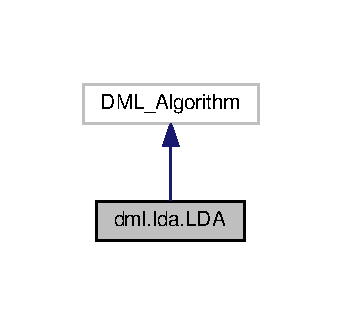
\includegraphics[width=164pt]{classdml_1_1lda_1_1LDA__inherit__graph}
\end{center}
\end{figure}


Collaboration diagram for dml.\+lda.\+L\+DA\+:
\nopagebreak
\begin{figure}[H]
\begin{center}
\leavevmode
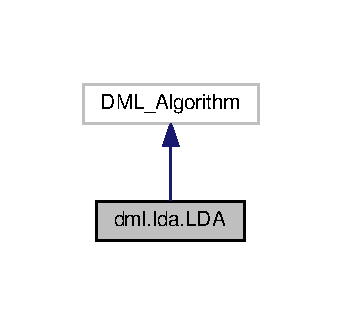
\includegraphics[width=164pt]{classdml_1_1lda_1_1LDA__coll__graph}
\end{center}
\end{figure}
\subsection*{Public Member Functions}
\begin{DoxyCompactItemize}
\item 
def {\bfseries \+\_\+\+\_\+init\+\_\+\+\_\+} (self, num\+\_\+dims=None, thres=None)\hypertarget{classdml_1_1lda_1_1LDA_a4e8e0793e2fdc34e9c3a2c8b2fd7dd15}{}\label{classdml_1_1lda_1_1LDA_a4e8e0793e2fdc34e9c3a2c8b2fd7dd15}

\item 
def \hyperlink{classdml_1_1lda_1_1LDA_a345bb18e92b9727b1835140cfb06bcf1}{transformer} (self)
\item 
def \hyperlink{classdml_1_1lda_1_1LDA_a34eac5a05ca665b60b01ecbbd7a97594}{metadata} (self)
\item 
def \hyperlink{classdml_1_1lda_1_1LDA_accd3f3321e39567e82f454228f592ab7}{fit} (self, X, y)
\item 
def {\bfseries transform} (self, X=None)\hypertarget{classdml_1_1lda_1_1LDA_a884b425003801e1978b5d56102b74ae6}{}\label{classdml_1_1lda_1_1LDA_a884b425003801e1978b5d56102b74ae6}

\end{DoxyCompactItemize}
\subsection*{Public Attributes}
\begin{DoxyCompactItemize}
\item 
{\bfseries nd\+\_\+init}\hypertarget{classdml_1_1lda_1_1LDA_afb68b0d3ab356c8c838ad35e3770c15c}{}\label{classdml_1_1lda_1_1LDA_afb68b0d3ab356c8c838ad35e3770c15c}

\item 
{\bfseries thres\+\_\+init}\hypertarget{classdml_1_1lda_1_1LDA_afe159730f871a6d9580b4a45806534ab}{}\label{classdml_1_1lda_1_1LDA_afe159730f871a6d9580b4a45806534ab}

\item 
{\bfseries nd\+\_\+}\hypertarget{classdml_1_1lda_1_1LDA_ae892ecd60e8720d3ac6383d85fca9487}{}\label{classdml_1_1lda_1_1LDA_ae892ecd60e8720d3ac6383d85fca9487}

\item 
{\bfseries acum\+\_\+eig\+\_\+}\hypertarget{classdml_1_1lda_1_1LDA_a2f098dcea1cf5f14733fcc6c49d7bc20}{}\label{classdml_1_1lda_1_1LDA_a2f098dcea1cf5f14733fcc6c49d7bc20}

\item 
{\bfseries X\+\_\+}\hypertarget{classdml_1_1lda_1_1LDA_ab21d96384e8ceca15a1cfae330917823}{}\label{classdml_1_1lda_1_1LDA_ab21d96384e8ceca15a1cfae330917823}

\item 
{\bfseries y\+\_\+}\hypertarget{classdml_1_1lda_1_1LDA_a1ee0f4abb92ce06808a92884933ac8e4}{}\label{classdml_1_1lda_1_1LDA_a1ee0f4abb92ce06808a92884933ac8e4}

\item 
{\bfseries d\+\_\+}\hypertarget{classdml_1_1lda_1_1LDA_ae4cfe2bc996e198f39fbae6272964d16}{}\label{classdml_1_1lda_1_1LDA_ae4cfe2bc996e198f39fbae6272964d16}

\item 
{\bfseries num\+\_\+dims}\hypertarget{classdml_1_1lda_1_1LDA_a0aa241704febbe5cce652192d054cc63}{}\label{classdml_1_1lda_1_1LDA_a0aa241704febbe5cce652192d054cc63}

\item 
{\bfseries thres}\hypertarget{classdml_1_1lda_1_1LDA_ac9bc7c47b10d413123e77b7b9d13e1c2}{}\label{classdml_1_1lda_1_1LDA_ac9bc7c47b10d413123e77b7b9d13e1c2}

\item 
{\bfseries sklda}\hypertarget{classdml_1_1lda_1_1LDA_ac93c9985f8872b8bf243671e07e3fa58}{}\label{classdml_1_1lda_1_1LDA_ac93c9985f8872b8bf243671e07e3fa58}

\item 
{\bfseries explained\+\_\+variance}\hypertarget{classdml_1_1lda_1_1LDA_a4848f91c654e62673865495473b93bb9}{}\label{classdml_1_1lda_1_1LDA_a4848f91c654e62673865495473b93bb9}

\item 
{\bfseries acum\+\_\+variance}\hypertarget{classdml_1_1lda_1_1LDA_aaf62c7f8712f45f2d981a8acdcf473eb}{}\label{classdml_1_1lda_1_1LDA_aaf62c7f8712f45f2d981a8acdcf473eb}

\item 
{\bfseries L\+\_\+}\hypertarget{classdml_1_1lda_1_1LDA_ad5c23356042d60aea6ce93a4397fd2ed}{}\label{classdml_1_1lda_1_1LDA_ad5c23356042d60aea6ce93a4397fd2ed}

\end{DoxyCompactItemize}


\subsection{Detailed Description}
\begin{DoxyVerb}Linear Discriminant Analysis (LDA).

A distance metric learning algorithm for supervised dimensionality reduction, maximizing the ratio of variances between classes and within classes.
This class is a wrapper for :class:`~sklearn.discriminant_analysis.LinearDiscriminantAnalysis`.

Parameters
----------

num_dims : int, default=None

    Number of components (< n_classes - 1) for dimensionality reduction. If None, it will be taken as n_classes - 1. Ignored if thres is provided.

thres : float

    Fraction of variability to keep, from 0 to 1. Data dimension will be reduced until the lowest dimension that keeps 'thres' explained variance.
\end{DoxyVerb}
 

\subsection{Member Function Documentation}
\index{dml\+::lda\+::\+L\+DA@{dml\+::lda\+::\+L\+DA}!fit@{fit}}
\index{fit@{fit}!dml\+::lda\+::\+L\+DA@{dml\+::lda\+::\+L\+DA}}
\subsubsection[{\texorpdfstring{fit(self, X, y)}{fit(self, X, y)}}]{\setlength{\rightskip}{0pt plus 5cm}def dml.\+lda.\+L\+D\+A.\+fit (
\begin{DoxyParamCaption}
\item[{}]{self, }
\item[{}]{X, }
\item[{}]{y}
\end{DoxyParamCaption}
)}\hypertarget{classdml_1_1lda_1_1LDA_accd3f3321e39567e82f454228f592ab7}{}\label{classdml_1_1lda_1_1LDA_accd3f3321e39567e82f454228f592ab7}
\begin{DoxyVerb}Fit the model from the data in X and the labels in y.

Parameters
----------
X : array-like, shape (N x d)
    Training vector, where N is the number of samples, and d is the number of features.

y : array-like, shape (N)
    Labels vector, where N is the number of samples.

Returns
-------
self : object
    Returns the instance itself.
\end{DoxyVerb}
 \index{dml\+::lda\+::\+L\+DA@{dml\+::lda\+::\+L\+DA}!metadata@{metadata}}
\index{metadata@{metadata}!dml\+::lda\+::\+L\+DA@{dml\+::lda\+::\+L\+DA}}
\subsubsection[{\texorpdfstring{metadata(self)}{metadata(self)}}]{\setlength{\rightskip}{0pt plus 5cm}def dml.\+lda.\+L\+D\+A.\+metadata (
\begin{DoxyParamCaption}
\item[{}]{self}
\end{DoxyParamCaption}
)}\hypertarget{classdml_1_1lda_1_1LDA_a34eac5a05ca665b60b01ecbbd7a97594}{}\label{classdml_1_1lda_1_1LDA_a34eac5a05ca665b60b01ecbbd7a97594}
\begin{DoxyVerb}Obtains algorithm metadata.

Returns
-------
meta : A dictionary with the following metadata:
    acum_eig : eigenvalue rate accumulated in the learned output respect to the total dimension.

    num_dims : dimension of the reduced data.
\end{DoxyVerb}
 \index{dml\+::lda\+::\+L\+DA@{dml\+::lda\+::\+L\+DA}!transformer@{transformer}}
\index{transformer@{transformer}!dml\+::lda\+::\+L\+DA@{dml\+::lda\+::\+L\+DA}}
\subsubsection[{\texorpdfstring{transformer(self)}{transformer(self)}}]{\setlength{\rightskip}{0pt plus 5cm}def dml.\+lda.\+L\+D\+A.\+transformer (
\begin{DoxyParamCaption}
\item[{}]{self}
\end{DoxyParamCaption}
)}\hypertarget{classdml_1_1lda_1_1LDA_a345bb18e92b9727b1835140cfb06bcf1}{}\label{classdml_1_1lda_1_1LDA_a345bb18e92b9727b1835140cfb06bcf1}
\begin{DoxyVerb}Obtains the learned projection.

Returns
-------
L : (d'xd) matrix, where d' is the desired output dimension and d is the number of features.
\end{DoxyVerb}
 

The documentation for this class was generated from the following file\+:\begin{DoxyCompactItemize}
\item 
dml/lda.\+pyx\end{DoxyCompactItemize}

\hypertarget{classdml_1_1ldml_1_1LDML}{}\section{dml.\+ldml.\+L\+D\+ML Class Reference}
\label{classdml_1_1ldml_1_1LDML}\index{dml.\+ldml.\+L\+D\+ML@{dml.\+ldml.\+L\+D\+ML}}


Inheritance diagram for dml.\+ldml.\+L\+D\+ML\+:
\nopagebreak
\begin{figure}[H]
\begin{center}
\leavevmode
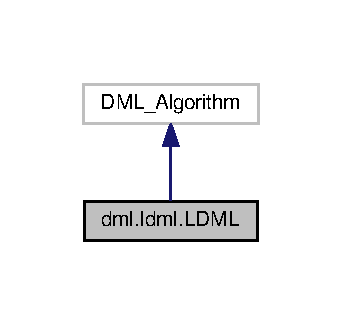
\includegraphics[width=164pt]{classdml_1_1ldml_1_1LDML__inherit__graph}
\end{center}
\end{figure}


Collaboration diagram for dml.\+ldml.\+L\+D\+ML\+:
\nopagebreak
\begin{figure}[H]
\begin{center}
\leavevmode
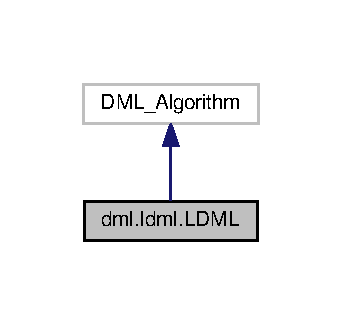
\includegraphics[width=164pt]{classdml_1_1ldml_1_1LDML__coll__graph}
\end{center}
\end{figure}
\subsection*{Public Member Functions}
\begin{DoxyCompactItemize}
\item 
def {\bfseries \+\_\+\+\_\+init\+\_\+\+\_\+} (self, num\+\_\+dims=None, b=1e-\/3, learning\+\_\+rate=\char`\"{}adaptive\char`\"{}, eta0=0.\+3, initial\+\_\+metric=\+None, max\+\_\+iter=10, prec=1e-\/3, tol=1e-\/3, descent\+\_\+method=\char`\"{}\+S\+D\+P\char`\"{}, eta\+\_\+thres=1e-\/14, learn\+\_\+inc=1.\+01, learn\+\_\+dec=0.\+5)\hypertarget{classdml_1_1ldml_1_1LDML_ab8de1c7e11f0341abf103e201fadc097}{}\label{classdml_1_1ldml_1_1LDML_ab8de1c7e11f0341abf103e201fadc097}

\item 
def \hyperlink{classdml_1_1ldml_1_1LDML_aff301dec555f6cba2967d55efa950385}{metadata} (self)
\item 
def \hyperlink{classdml_1_1ldml_1_1LDML_a4fdf9da7a2b97aefe931ac02867b56df}{metric} (self)
\item 
def \hyperlink{classdml_1_1ldml_1_1LDML_a8b6f427cf624e68ffda7d703189f7072}{fit} (self, X, y)
\end{DoxyCompactItemize}
\subsection*{Public Attributes}
\begin{DoxyCompactItemize}
\item 
{\bfseries num\+\_\+dims\+\_\+}\hypertarget{classdml_1_1ldml_1_1LDML_a92091ae46b34a7316152076303542c0e}{}\label{classdml_1_1ldml_1_1LDML_a92091ae46b34a7316152076303542c0e}

\item 
{\bfseries initial\+\_\+}\hypertarget{classdml_1_1ldml_1_1LDML_a65faa54129b0d4e94ed58f1fad311d79}{}\label{classdml_1_1ldml_1_1LDML_a65faa54129b0d4e94ed58f1fad311d79}

\item 
{\bfseries max\+\_\+it\+\_\+}\hypertarget{classdml_1_1ldml_1_1LDML_ace75c89206a7fec7ed40a6a5d4ae03bb}{}\label{classdml_1_1ldml_1_1LDML_ace75c89206a7fec7ed40a6a5d4ae03bb}

\item 
{\bfseries eta\+\_\+}\hypertarget{classdml_1_1ldml_1_1LDML_aa5b8ce9ef16ac45aca504fcb77205157}{}\label{classdml_1_1ldml_1_1LDML_aa5b8ce9ef16ac45aca504fcb77205157}

\item 
{\bfseries eta0\+\_\+}\hypertarget{classdml_1_1ldml_1_1LDML_a867a3e8ac0e4a1075ac6ef05dabbcc22}{}\label{classdml_1_1ldml_1_1LDML_a867a3e8ac0e4a1075ac6ef05dabbcc22}

\item 
{\bfseries learning\+\_\+}\hypertarget{classdml_1_1ldml_1_1LDML_a3ddcd42ccc6610f475f736809cf195e1}{}\label{classdml_1_1ldml_1_1LDML_a3ddcd42ccc6610f475f736809cf195e1}

\item 
{\bfseries adaptive\+\_\+}\hypertarget{classdml_1_1ldml_1_1LDML_a86cddd4714d6a5f102c5db65b143a872}{}\label{classdml_1_1ldml_1_1LDML_a86cddd4714d6a5f102c5db65b143a872}

\item 
{\bfseries method\+\_\+}\hypertarget{classdml_1_1ldml_1_1LDML_a2071b8f3e4d4dba544fea542276d2aa5}{}\label{classdml_1_1ldml_1_1LDML_a2071b8f3e4d4dba544fea542276d2aa5}

\item 
{\bfseries eps\+\_\+}\hypertarget{classdml_1_1ldml_1_1LDML_a1d4f83ffa0c39ff1cc6f67870ce39852}{}\label{classdml_1_1ldml_1_1LDML_a1d4f83ffa0c39ff1cc6f67870ce39852}

\item 
{\bfseries tol\+\_\+}\hypertarget{classdml_1_1ldml_1_1LDML_a03ec2b6101ff3fc25dcfc9f24352346c}{}\label{classdml_1_1ldml_1_1LDML_a03ec2b6101ff3fc25dcfc9f24352346c}

\item 
{\bfseries etamin\+\_\+}\hypertarget{classdml_1_1ldml_1_1LDML_a9f80238138eb06019729d660c9c7531e}{}\label{classdml_1_1ldml_1_1LDML_a9f80238138eb06019729d660c9c7531e}

\item 
{\bfseries l\+\_\+inc\+\_\+}\hypertarget{classdml_1_1ldml_1_1LDML_af0d8c3d7158f1912437dc2169f23af73}{}\label{classdml_1_1ldml_1_1LDML_af0d8c3d7158f1912437dc2169f23af73}

\item 
{\bfseries l\+\_\+dec\+\_\+}\hypertarget{classdml_1_1ldml_1_1LDML_a7fddbc6d780fd0477dcf1f847a0fc2b0}{}\label{classdml_1_1ldml_1_1LDML_a7fddbc6d780fd0477dcf1f847a0fc2b0}

\item 
{\bfseries b\+\_\+}\hypertarget{classdml_1_1ldml_1_1LDML_a3c099278f02af677357425d78a1a82d1}{}\label{classdml_1_1ldml_1_1LDML_a3c099278f02af677357425d78a1a82d1}

\item 
{\bfseries num\+\_\+its\+\_\+}\hypertarget{classdml_1_1ldml_1_1LDML_ac975d7033641c7ae0ed64b9aaab07fbc}{}\label{classdml_1_1ldml_1_1LDML_ac975d7033641c7ae0ed64b9aaab07fbc}

\item 
{\bfseries initial\+\_\+error\+\_\+}\hypertarget{classdml_1_1ldml_1_1LDML_a0c326ce8a1622f23df51dc3ecfd5ad8b}{}\label{classdml_1_1ldml_1_1LDML_a0c326ce8a1622f23df51dc3ecfd5ad8b}

\item 
{\bfseries final\+\_\+error\+\_\+}\hypertarget{classdml_1_1ldml_1_1LDML_a5e9d05a17dab342e58fca27e65642d93}{}\label{classdml_1_1ldml_1_1LDML_a5e9d05a17dab342e58fca27e65642d93}

\item 
{\bfseries d\+\_\+}\hypertarget{classdml_1_1ldml_1_1LDML_ad4206379ee9fd398911e1d0475d7b4e2}{}\label{classdml_1_1ldml_1_1LDML_ad4206379ee9fd398911e1d0475d7b4e2}

\item 
{\bfseries nd\+\_\+}\hypertarget{classdml_1_1ldml_1_1LDML_a71f103f58592b4571454ea90902493dc}{}\label{classdml_1_1ldml_1_1LDML_a71f103f58592b4571454ea90902493dc}

\item 
{\bfseries X\+\_\+}\hypertarget{classdml_1_1ldml_1_1LDML_a0d00fb756d9cbf6e7a7addd2c10dee27}{}\label{classdml_1_1ldml_1_1LDML_a0d00fb756d9cbf6e7a7addd2c10dee27}

\item 
{\bfseries y\+\_\+}\hypertarget{classdml_1_1ldml_1_1LDML_aaf8af00e81bc57266aaaa0400f5a851b}{}\label{classdml_1_1ldml_1_1LDML_aaf8af00e81bc57266aaaa0400f5a851b}

\item 
{\bfseries M\+\_\+}\hypertarget{classdml_1_1ldml_1_1LDML_a51c3f7b29fca79d999f62b717bd17784}{}\label{classdml_1_1ldml_1_1LDML_a51c3f7b29fca79d999f62b717bd17784}

\end{DoxyCompactItemize}


\subsection{Detailed Description}
\begin{DoxyVerb}Logistic Discriminant Metric Learning (LDML).

Distance Metric Learning through the likelihood maximization of a logistic based probability distribution.

Parameters
----------

num_dims : int, default=None.

    Number of dimensions for dimensionality reduction. Not supported yet.

b : float, default=1e-3

    Logistic function positive threshold.

learning_rate : string, default='adaptive'

    Type of learning rate update for gradient descent. Possible values are:

    - 'adaptive' : the learning rate will increase if the gradient step is succesful, else it will decrease.

    - 'constant' : the learning rate will be constant during all the gradient steps.

eta0 : float, default=0.3

    The initial value for learning rate.

initial_metric : 2D-Array or Matrix (d x d), or string, default=None.

    If array or matrix, it must be a positive semidefinite matrix with the starting metric for gradient descent, where d is the number of features.
    If None, euclidean distance will be used. If a string, the following values are allowed:

    - 'euclidean' : the euclidean distance.

    - 'scale' : a diagonal matrix that normalizes each attribute according to its range will be used.

max_iter : int, default=10

    Maximum number of iterations of gradient descent.

prec : float, default=1e-3

    Precision stop criterion (gradient norm).

tol : float, default=1e-3

    Tolerance stop criterion (difference between two iterations)

descent_method : string, default='SDP'

    The descent method to use. Allowed values are:

    - 'SDP' : semidefinite programming, consisting of gradient descent with projections onto the PSD cone.

eta_thres : float, default=1e-14

    A learning rate threshold stop criterion.

learn_inc : float, default=1.01

    Increase factor for learning rate. Ignored if learning_rate is not 'adaptive'.

learn_dec : float, default=0.5

    Decrease factor for learning rate. Ignored if learning_rate is not 'adaptive'.


References
----------
    Matthieu Guillaumin, Jakob Verbeek and Cordelia Schmid. “Is that you? Metric learning approaches
    for face identification”. In: Computer Vision, 2009 IEEE 12th international conference on. IEEE.
    2009, pages 498-505.
\end{DoxyVerb}
 

\subsection{Member Function Documentation}
\index{dml\+::ldml\+::\+L\+D\+ML@{dml\+::ldml\+::\+L\+D\+ML}!fit@{fit}}
\index{fit@{fit}!dml\+::ldml\+::\+L\+D\+ML@{dml\+::ldml\+::\+L\+D\+ML}}
\subsubsection[{\texorpdfstring{fit(self, X, y)}{fit(self, X, y)}}]{\setlength{\rightskip}{0pt plus 5cm}def dml.\+ldml.\+L\+D\+M\+L.\+fit (
\begin{DoxyParamCaption}
\item[{}]{self, }
\item[{}]{X, }
\item[{}]{y}
\end{DoxyParamCaption}
)}\hypertarget{classdml_1_1ldml_1_1LDML_a8b6f427cf624e68ffda7d703189f7072}{}\label{classdml_1_1ldml_1_1LDML_a8b6f427cf624e68ffda7d703189f7072}
\begin{DoxyVerb}Fit the model from the data in X and the labels in y.

Parameters
----------
X : array-like, shape (N x d)
    Training vector, where N is the number of samples, and d is the number of features.

y : array-like, shape (N)
    Labels vector, where N is the number of samples.

Returns
-------
self : object
    Returns the instance itself.
\end{DoxyVerb}
 \index{dml\+::ldml\+::\+L\+D\+ML@{dml\+::ldml\+::\+L\+D\+ML}!metadata@{metadata}}
\index{metadata@{metadata}!dml\+::ldml\+::\+L\+D\+ML@{dml\+::ldml\+::\+L\+D\+ML}}
\subsubsection[{\texorpdfstring{metadata(self)}{metadata(self)}}]{\setlength{\rightskip}{0pt plus 5cm}def dml.\+ldml.\+L\+D\+M\+L.\+metadata (
\begin{DoxyParamCaption}
\item[{}]{self}
\end{DoxyParamCaption}
)}\hypertarget{classdml_1_1ldml_1_1LDML_aff301dec555f6cba2967d55efa950385}{}\label{classdml_1_1ldml_1_1LDML_aff301dec555f6cba2967d55efa950385}
\begin{DoxyVerb}Obtains algorithm metadata.

Returns
-------
meta : A dictionary with the following metadata:
    - 'num_iters' : Number of iterations that the descent method took.

    - 'initial_error' : Initial value of the objective function.

    - 'final_error' : Final value of the objective function.
\end{DoxyVerb}
 \index{dml\+::ldml\+::\+L\+D\+ML@{dml\+::ldml\+::\+L\+D\+ML}!metric@{metric}}
\index{metric@{metric}!dml\+::ldml\+::\+L\+D\+ML@{dml\+::ldml\+::\+L\+D\+ML}}
\subsubsection[{\texorpdfstring{metric(self)}{metric(self)}}]{\setlength{\rightskip}{0pt plus 5cm}def dml.\+ldml.\+L\+D\+M\+L.\+metric (
\begin{DoxyParamCaption}
\item[{}]{self}
\end{DoxyParamCaption}
)}\hypertarget{classdml_1_1ldml_1_1LDML_a4fdf9da7a2b97aefe931ac02867b56df}{}\label{classdml_1_1ldml_1_1LDML_a4fdf9da7a2b97aefe931ac02867b56df}
\begin{DoxyVerb}Obtains the learned metric.

Returns
-------
M : (dxd) positive semidefinite matrix, where d is the number of features.
\end{DoxyVerb}
 

The documentation for this class was generated from the following file\+:\begin{DoxyCompactItemize}
\item 
dml/ldml.\+pyx\end{DoxyCompactItemize}

\hypertarget{classdml_1_1lmnn_1_1LMNN}{}\section{dml.\+lmnn.\+L\+M\+NN Class Reference}
\label{classdml_1_1lmnn_1_1LMNN}\index{dml.\+lmnn.\+L\+M\+NN@{dml.\+lmnn.\+L\+M\+NN}}


Inheritance diagram for dml.\+lmnn.\+L\+M\+NN\+:
\nopagebreak
\begin{figure}[H]
\begin{center}
\leavevmode
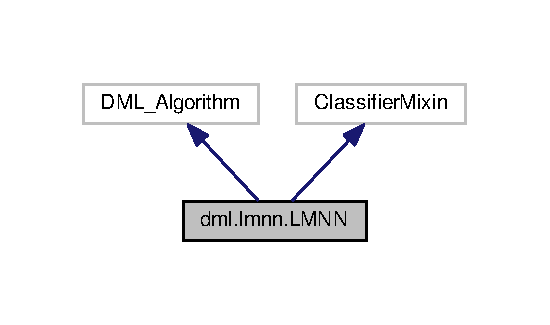
\includegraphics[width=264pt]{classdml_1_1lmnn_1_1LMNN__inherit__graph}
\end{center}
\end{figure}


Collaboration diagram for dml.\+lmnn.\+L\+M\+NN\+:
\nopagebreak
\begin{figure}[H]
\begin{center}
\leavevmode
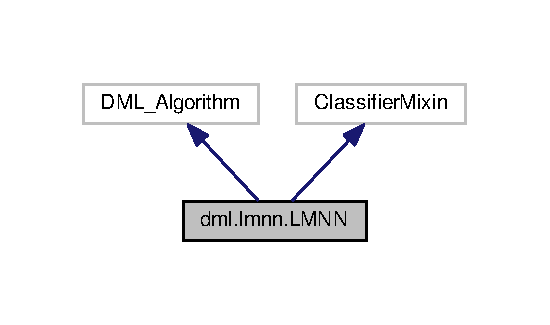
\includegraphics[width=264pt]{classdml_1_1lmnn_1_1LMNN__coll__graph}
\end{center}
\end{figure}
\subsection*{Public Member Functions}
\begin{DoxyCompactItemize}
\item 
def {\bfseries \+\_\+\+\_\+init\+\_\+\+\_\+} (self, num\+\_\+dims=None, learning\+\_\+rate=\char`\"{}adaptive\char`\"{}, eta0=0.\+3, initial\+\_\+metric=None, max\+\_\+iter=100, prec=1e-\/8, tol=1e-\/8, k=3, mu=0.\+5, soft\+\_\+comp\+\_\+interval=1, learn\+\_\+inc=1.\+01, learn\+\_\+dec=0.\+5, eta\+\_\+thres=1e-\/14, solver=\char`\"{}\+S\+D\+P\char`\"{})\hypertarget{classdml_1_1lmnn_1_1LMNN_ab2ab17715d79b9c53b7a414fc8d7a347}{}\label{classdml_1_1lmnn_1_1LMNN_ab2ab17715d79b9c53b7a414fc8d7a347}

\item 
def \hyperlink{classdml_1_1lmnn_1_1LMNN_a112eee35ecdb3476172f4ac4ad2a4c40}{metadata} (self)
\item 
def \hyperlink{classdml_1_1lmnn_1_1LMNN_ac69c9741352a38851e85172b25766af6}{fit} (self, X, y)
\item 
def \hyperlink{classdml_1_1lmnn_1_1LMNN_a06e4bb50c7f50b7e6bac689743198b32}{predict} (self, X=None)
\end{DoxyCompactItemize}
\subsection*{Public Attributes}
\begin{DoxyCompactItemize}
\item 
{\bfseries num\+\_\+dims\+\_\+}\hypertarget{classdml_1_1lmnn_1_1LMNN_afcdbb5898f7f30b6625a4ae89e253064}{}\label{classdml_1_1lmnn_1_1LMNN_afcdbb5898f7f30b6625a4ae89e253064}

\item 
{\bfseries M0\+\_\+}\hypertarget{classdml_1_1lmnn_1_1LMNN_a6b70e7d61aa51b093fb0ce59d12584b9}{}\label{classdml_1_1lmnn_1_1LMNN_a6b70e7d61aa51b093fb0ce59d12584b9}

\item 
{\bfseries max\+\_\+it\+\_\+}\hypertarget{classdml_1_1lmnn_1_1LMNN_aee92343b4aaf79834b86de6d36a35d4d}{}\label{classdml_1_1lmnn_1_1LMNN_aee92343b4aaf79834b86de6d36a35d4d}

\item 
{\bfseries eta0\+\_\+}\hypertarget{classdml_1_1lmnn_1_1LMNN_af54000da768085101c9b5d93c08b3e25}{}\label{classdml_1_1lmnn_1_1LMNN_af54000da768085101c9b5d93c08b3e25}

\item 
{\bfseries eta\+\_\+}\hypertarget{classdml_1_1lmnn_1_1LMNN_ab1df778b4a67aceb70c3cf6a8c79ae9f}{}\label{classdml_1_1lmnn_1_1LMNN_ab1df778b4a67aceb70c3cf6a8c79ae9f}

\item 
{\bfseries learning\+\_\+}\hypertarget{classdml_1_1lmnn_1_1LMNN_ac6a4848ad7fb33bba32ffdb484d2948a}{}\label{classdml_1_1lmnn_1_1LMNN_ac6a4848ad7fb33bba32ffdb484d2948a}

\item 
{\bfseries adaptive\+\_\+}\hypertarget{classdml_1_1lmnn_1_1LMNN_a70f5a8d225cc5d65d4b870927ce944d3}{}\label{classdml_1_1lmnn_1_1LMNN_a70f5a8d225cc5d65d4b870927ce944d3}

\item 
{\bfseries eps\+\_\+}\hypertarget{classdml_1_1lmnn_1_1LMNN_a439da790aa374144e4eaca184b744f1b}{}\label{classdml_1_1lmnn_1_1LMNN_a439da790aa374144e4eaca184b744f1b}

\item 
{\bfseries tol\+\_\+}\hypertarget{classdml_1_1lmnn_1_1LMNN_a3b6c6b17a5ffab3a9d8614b0c48bdfea}{}\label{classdml_1_1lmnn_1_1LMNN_a3b6c6b17a5ffab3a9d8614b0c48bdfea}

\item 
{\bfseries mu\+\_\+}\hypertarget{classdml_1_1lmnn_1_1LMNN_a32684b7381e1f8c440583426546e9fbd}{}\label{classdml_1_1lmnn_1_1LMNN_a32684b7381e1f8c440583426546e9fbd}

\item 
{\bfseries k\+\_\+}\hypertarget{classdml_1_1lmnn_1_1LMNN_a2d5495135fa0b1810a67aa321a1e1832}{}\label{classdml_1_1lmnn_1_1LMNN_a2d5495135fa0b1810a67aa321a1e1832}

\item 
{\bfseries soft\+\_\+comp\+\_\+interval\+\_\+}\hypertarget{classdml_1_1lmnn_1_1LMNN_aaa7bffb95d46970b92c898e4b367a462}{}\label{classdml_1_1lmnn_1_1LMNN_aaa7bffb95d46970b92c898e4b367a462}

\item 
{\bfseries l\+\_\+inc\+\_\+}\hypertarget{classdml_1_1lmnn_1_1LMNN_a50ce218d4840e05839eb84b4ecc8c1ca}{}\label{classdml_1_1lmnn_1_1LMNN_a50ce218d4840e05839eb84b4ecc8c1ca}

\item 
{\bfseries l\+\_\+dec\+\_\+}\hypertarget{classdml_1_1lmnn_1_1LMNN_ad3c3dd709e5e8d41785847f3b6ef2d7d}{}\label{classdml_1_1lmnn_1_1LMNN_ad3c3dd709e5e8d41785847f3b6ef2d7d}

\item 
{\bfseries etamin\+\_\+}\hypertarget{classdml_1_1lmnn_1_1LMNN_a1fc05f5581985840ce49c1207ca45315}{}\label{classdml_1_1lmnn_1_1LMNN_a1fc05f5581985840ce49c1207ca45315}

\item 
{\bfseries solver\+\_\+}\hypertarget{classdml_1_1lmnn_1_1LMNN_aa4b40032aa6c3da2c3b20da8038d66c1}{}\label{classdml_1_1lmnn_1_1LMNN_aa4b40032aa6c3da2c3b20da8038d66c1}

\item 
{\bfseries num\+\_\+its\+\_\+}\hypertarget{classdml_1_1lmnn_1_1LMNN_ad916f82a407b90af4db2bc5d47222cdf}{}\label{classdml_1_1lmnn_1_1LMNN_ad916f82a407b90af4db2bc5d47222cdf}

\item 
{\bfseries initial\+\_\+error\+\_\+}\hypertarget{classdml_1_1lmnn_1_1LMNN_aa398128acb2b0df7b694bbc212d526c3}{}\label{classdml_1_1lmnn_1_1LMNN_aa398128acb2b0df7b694bbc212d526c3}

\item 
{\bfseries final\+\_\+error\+\_\+}\hypertarget{classdml_1_1lmnn_1_1LMNN_a9a24b07e143896e64d6879761bc3a897}{}\label{classdml_1_1lmnn_1_1LMNN_a9a24b07e143896e64d6879761bc3a897}

\item 
{\bfseries target\+\_\+neighbors\+\_\+}\hypertarget{classdml_1_1lmnn_1_1LMNN_a12d7f9b1bbb7730f617cfd618cfd3a91}{}\label{classdml_1_1lmnn_1_1LMNN_a12d7f9b1bbb7730f617cfd618cfd3a91}

\item 
{\bfseries M\+\_\+}\hypertarget{classdml_1_1lmnn_1_1LMNN_a5f5322f8e73abd730cf68689f04eefab}{}\label{classdml_1_1lmnn_1_1LMNN_a5f5322f8e73abd730cf68689f04eefab}

\item 
{\bfseries y\+\_\+}\hypertarget{classdml_1_1lmnn_1_1LMNN_a910e52ed27c964b56a30c34b01e7e21e}{}\label{classdml_1_1lmnn_1_1LMNN_a910e52ed27c964b56a30c34b01e7e21e}

\item 
{\bfseries d\+\_\+}\hypertarget{classdml_1_1lmnn_1_1LMNN_ad286d75fd9c06a901d56eadee26a64e1}{}\label{classdml_1_1lmnn_1_1LMNN_ad286d75fd9c06a901d56eadee26a64e1}

\item 
{\bfseries nd\+\_\+}\hypertarget{classdml_1_1lmnn_1_1LMNN_a69cc3e9fd8cda8d92c20f8505282dea1}{}\label{classdml_1_1lmnn_1_1LMNN_a69cc3e9fd8cda8d92c20f8505282dea1}

\item 
{\bfseries L\+\_\+}\hypertarget{classdml_1_1lmnn_1_1LMNN_a96df0b36af8bafc77b7f0b7c522417e0}{}\label{classdml_1_1lmnn_1_1LMNN_a96df0b36af8bafc77b7f0b7c522417e0}

\item 
{\bfseries X\+\_\+}\hypertarget{classdml_1_1lmnn_1_1LMNN_a4c5e97d524842b7ec2ca0d9ea65f9e04}{}\label{classdml_1_1lmnn_1_1LMNN_a4c5e97d524842b7ec2ca0d9ea65f9e04}

\end{DoxyCompactItemize}


\subsection{Detailed Description}
\begin{DoxyVerb}Large Margin Nearest Neighbors (LMNN)

A distance metric learning algorithm that obtains a metric with target neighbors as near as possible and impostors as far as possible

Parameters
----------

num_dims : int, default=None

    Desired value for dimensionality reduction. Ignored if solver is 'SDP'.

learning_rate : string, default='adaptive'

    Type of learning rate update for gradient descent. Possible values are:

    - 'adaptive' : the learning rate will increase if the gradient step is succesful, else it will decrease.

    - 'constant' : the learning rate will be constant during all the gradient steps.

eta0 : int, default=0.3

    The initial value for learning rate.

initial_metric : 2D-Array or Matrix (d' x d), or string, default=None.

    If array or matrix, and solver is SDP, it must be a positive semidefinite matrix with the starting metric (d x d) for gradient descent, where d is the number of features.
    If None, euclidean distance will be used. If a string, the following values are allowed:

    - 'euclidean' : the euclidean distance.

    - 'scale' : a diagonal matrix that normalizes each attribute according to its range will be used.

    If solver is SGD, then the array or matrix will represent a linear map (d' x d), where d' is the dimension provided in num_dims.

max_iter : int, default=100

    Maximum number of iterations of gradient descent.

prec : float, default=1e-8

    Precision stop criterion (gradient norm).

tol : float, default=1e-8

    Tolerance stop criterion (difference between two iterations)

k : int, default=3

    Number of target neighbors to take. If this algorithm is used for nearest neighbors classification, a good choice is
    to take k as the number of neighbors.

mu : float, default=0.5

    The weight of the push error in the minimization algorithm. The objective function is composed of a push error, given by the impostors,
    with weight mu, and a pull error, given by the target neighbors, with weight (1-mu). It must be between 0.0 and 1.0.

soft_comp_interval : int, default=1

    Intervals of soft computation. The soft computation relaxes the gradient descent conditions, but makes the algorithm more efficient.
    This value provides the length of a soft computation interval. After soft_comp_interval iterations of gradient descent, a complete
    gradient step is performed.

learn_inc : float, default=1.01

    Increase factor for learning rate. Ignored if learning_rate is not 'adaptive'.

learn_dec : float, default=0.5

    Decrease factor for learning rate. Ignored if learning_rate is not 'adaptive'.

eta_thres : float, default=1e-14

    A learning rate threshold stop criterion.

solver : string, default='SDP'

    The algorithm used for minimization. Allowed values are:

    - 'SDP' : semidefinite programming, consisting of gradient descent with projections onto the positive semidefinite cone.
              It learns a metric.

    - 'SGD' : stochastic gradient descent. It learns a linear transformer.

References
----------
    Kilian Q Weinberger and Lawrence K Saul. “Distance metric learning for large margin nearest
    neighbor classification”. In: Journal of Machine Learning Research 10.Feb (2009), pages 207-244.
\end{DoxyVerb}
 

\subsection{Member Function Documentation}
\index{dml\+::lmnn\+::\+L\+M\+NN@{dml\+::lmnn\+::\+L\+M\+NN}!fit@{fit}}
\index{fit@{fit}!dml\+::lmnn\+::\+L\+M\+NN@{dml\+::lmnn\+::\+L\+M\+NN}}
\subsubsection[{\texorpdfstring{fit(self, X, y)}{fit(self, X, y)}}]{\setlength{\rightskip}{0pt plus 5cm}def dml.\+lmnn.\+L\+M\+N\+N.\+fit (
\begin{DoxyParamCaption}
\item[{}]{self, }
\item[{}]{X, }
\item[{}]{y}
\end{DoxyParamCaption}
)}\hypertarget{classdml_1_1lmnn_1_1LMNN_ac69c9741352a38851e85172b25766af6}{}\label{classdml_1_1lmnn_1_1LMNN_ac69c9741352a38851e85172b25766af6}
\begin{DoxyVerb}Fit the model from the data in X and the labels in y.

Parameters
----------
X : array-like, shape (N x d)
    Training vector, where N is the number of samples, and d is the number of features.

y : array-like, shape (N)
    Labels vector, where N is the number of samples.

Returns
-------
self : object
    Returns the instance itself.
\end{DoxyVerb}
 \index{dml\+::lmnn\+::\+L\+M\+NN@{dml\+::lmnn\+::\+L\+M\+NN}!metadata@{metadata}}
\index{metadata@{metadata}!dml\+::lmnn\+::\+L\+M\+NN@{dml\+::lmnn\+::\+L\+M\+NN}}
\subsubsection[{\texorpdfstring{metadata(self)}{metadata(self)}}]{\setlength{\rightskip}{0pt plus 5cm}def dml.\+lmnn.\+L\+M\+N\+N.\+metadata (
\begin{DoxyParamCaption}
\item[{}]{self}
\end{DoxyParamCaption}
)}\hypertarget{classdml_1_1lmnn_1_1LMNN_a112eee35ecdb3476172f4ac4ad2a4c40}{}\label{classdml_1_1lmnn_1_1LMNN_a112eee35ecdb3476172f4ac4ad2a4c40}
\begin{DoxyVerb}Obtains algorithm metadata.

Returns
-------
meta : A dictionary with the following metadata:
    - num_iters : Number of iterations that the descent method took.

    - initial_error : Initial value of the objective function.

    - final_error : Final value of the objective function.
\end{DoxyVerb}
 \index{dml\+::lmnn\+::\+L\+M\+NN@{dml\+::lmnn\+::\+L\+M\+NN}!predict@{predict}}
\index{predict@{predict}!dml\+::lmnn\+::\+L\+M\+NN@{dml\+::lmnn\+::\+L\+M\+NN}}
\subsubsection[{\texorpdfstring{predict(self, X=\+None)}{predict(self, X=None)}}]{\setlength{\rightskip}{0pt plus 5cm}def dml.\+lmnn.\+L\+M\+N\+N.\+predict (
\begin{DoxyParamCaption}
\item[{}]{self, }
\item[{}]{X = {\ttfamily None}}
\end{DoxyParamCaption}
)}\hypertarget{classdml_1_1lmnn_1_1LMNN_a06e4bb50c7f50b7e6bac689743198b32}{}\label{classdml_1_1lmnn_1_1LMNN_a06e4bb50c7f50b7e6bac689743198b32}
\begin{DoxyVerb}Predict the class labels for the provided data, according to the LMNN energy method.

Parameters
----------
X : array-like, shape (N x d)

    Test samples. N is the number of samples and d the number of features. If None, training set will be used.

Returns
-------
y : array of shape (N)

    Class labels for each data sample.
\end{DoxyVerb}
 

The documentation for this class was generated from the following file\+:\begin{DoxyCompactItemize}
\item 
dml/lmnn.\+pyx\end{DoxyCompactItemize}

\hypertarget{classdml_1_1lsi_1_1LSI}{}\section{dml.\+lsi.\+L\+SI Class Reference}
\label{classdml_1_1lsi_1_1LSI}\index{dml.\+lsi.\+L\+SI@{dml.\+lsi.\+L\+SI}}


Inheritance diagram for dml.\+lsi.\+L\+SI\+:
\nopagebreak
\begin{figure}[H]
\begin{center}
\leavevmode
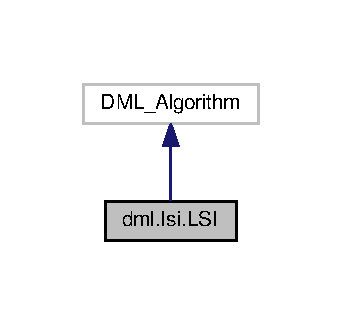
\includegraphics[width=164pt]{classdml_1_1lsi_1_1LSI__inherit__graph}
\end{center}
\end{figure}


Collaboration diagram for dml.\+lsi.\+L\+SI\+:
\nopagebreak
\begin{figure}[H]
\begin{center}
\leavevmode
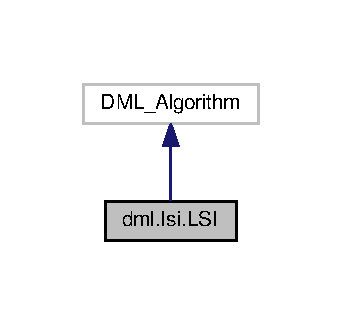
\includegraphics[width=164pt]{classdml_1_1lsi_1_1LSI__coll__graph}
\end{center}
\end{figure}
\subsection*{Public Member Functions}
\begin{DoxyCompactItemize}
\item 
def {\bfseries \+\_\+\+\_\+init\+\_\+\+\_\+} (self, initial\+\_\+metric=None, learning\+\_\+rate=\textquotesingle{}adaptive\textquotesingle{}, eta0=0.\+1, max\+\_\+iter=100, max\+\_\+proj\+\_\+iter=5000, itproj\+\_\+err=1e-\/3, err=1e-\/3, supervised=\+False)\hypertarget{classdml_1_1lsi_1_1LSI_ac7b6cb5c0c275e569cacaad9d10bd65f}{}\label{classdml_1_1lsi_1_1LSI_ac7b6cb5c0c275e569cacaad9d10bd65f}

\item 
def \hyperlink{classdml_1_1lsi_1_1LSI_aff08bb1d85ceb7815463dab942c874fe}{metric} (self)
\item 
def \hyperlink{classdml_1_1lsi_1_1LSI_a0b19b5b4c15e9ece71a6cfa99206450e}{metadata} (self)
\item 
def \hyperlink{classdml_1_1lsi_1_1LSI_abf52e31fccbbbb83b3f5ec8fcaeee27a}{fit} (self, X, side)
\item 
def {\bfseries label\+\_\+to\+\_\+similarity\+\_\+set} (y)\hypertarget{classdml_1_1lsi_1_1LSI_a8072dcc31d51a2942653c7d07be24d2c}{}\label{classdml_1_1lsi_1_1LSI_a8072dcc31d51a2942653c7d07be24d2c}

\item 
def {\bfseries f\+S1} (X, S, M, N, d, outers)\hypertarget{classdml_1_1lsi_1_1LSI_adf17afd3275593c0ce6ee6ea860ab32b}{}\label{classdml_1_1lsi_1_1LSI_adf17afd3275593c0ce6ee6ea860ab32b}

\item 
def {\bfseries f\+D1} (X, D, M, N, d, outers)\hypertarget{classdml_1_1lsi_1_1LSI_ab6ab40d92d222f31c12b2801005571c2}{}\label{classdml_1_1lsi_1_1LSI_ab6ab40d92d222f31c12b2801005571c2}

\item 
def {\bfseries fD} (X, D, M, N, d)\hypertarget{classdml_1_1lsi_1_1LSI_a9ffd83da171f9d5f5fabce573cd23cc3}{}\label{classdml_1_1lsi_1_1LSI_a9ffd83da171f9d5f5fabce573cd23cc3}

\item 
def {\bfseries fS} (X, S, M, N, d)\hypertarget{classdml_1_1lsi_1_1LSI_a599aa47db1a73be6cff23ec70c56c28c}{}\label{classdml_1_1lsi_1_1LSI_a599aa47db1a73be6cff23ec70c56c28c}

\item 
def {\bfseries grad\+\_\+projection} (grad1, grad2, d)\hypertarget{classdml_1_1lsi_1_1LSI_acce0d0074acf4c7406559d5155ccc4e7}{}\label{classdml_1_1lsi_1_1LSI_acce0d0074acf4c7406559d5155ccc4e7}

\end{DoxyCompactItemize}
\subsection*{Public Attributes}
\begin{DoxyCompactItemize}
\item 
{\bfseries M0\+\_\+}\hypertarget{classdml_1_1lsi_1_1LSI_a4a7b5fcb9211906739bc6624e9e0898e}{}\label{classdml_1_1lsi_1_1LSI_a4a7b5fcb9211906739bc6624e9e0898e}

\item 
{\bfseries eta0\+\_\+}\hypertarget{classdml_1_1lsi_1_1LSI_a5abbe8d95bf5d503b573952267b2e28d}{}\label{classdml_1_1lsi_1_1LSI_a5abbe8d95bf5d503b573952267b2e28d}

\item 
{\bfseries learning\+\_\+}\hypertarget{classdml_1_1lsi_1_1LSI_aa35166d1dfa8883f703b0a42d8fedb1f}{}\label{classdml_1_1lsi_1_1LSI_aa35166d1dfa8883f703b0a42d8fedb1f}

\item 
{\bfseries max\+\_\+it\+\_\+}\hypertarget{classdml_1_1lsi_1_1LSI_a4bb51eeeacaf2e7e64ab2e0dbc999781}{}\label{classdml_1_1lsi_1_1LSI_a4bb51eeeacaf2e7e64ab2e0dbc999781}

\item 
{\bfseries max\+\_\+projit\+\_\+}\hypertarget{classdml_1_1lsi_1_1LSI_a8cf51ca43d7e1417067c269936885189}{}\label{classdml_1_1lsi_1_1LSI_a8cf51ca43d7e1417067c269936885189}

\item 
{\bfseries itproj\+\_\+err\+\_\+}\hypertarget{classdml_1_1lsi_1_1LSI_afaef7cf510f97b2c759073eae68d1ef3}{}\label{classdml_1_1lsi_1_1LSI_afaef7cf510f97b2c759073eae68d1ef3}

\item 
{\bfseries err\+\_\+}\hypertarget{classdml_1_1lsi_1_1LSI_aa777e43a117aa59c54f1548296d74b10}{}\label{classdml_1_1lsi_1_1LSI_aa777e43a117aa59c54f1548296d74b10}

\item 
{\bfseries supv\+\_\+}\hypertarget{classdml_1_1lsi_1_1LSI_a9b85e6908563f1ec116ae6d5e4e19a5d}{}\label{classdml_1_1lsi_1_1LSI_a9b85e6908563f1ec116ae6d5e4e19a5d}

\item 
{\bfseries iterative\+\_\+projections\+\_\+conv\+\_\+exp\+\_\+}\hypertarget{classdml_1_1lsi_1_1LSI_a8f65b277e2118e12a5f2f0ad7d44a6d8}{}\label{classdml_1_1lsi_1_1LSI_a8f65b277e2118e12a5f2f0ad7d44a6d8}

\item 
{\bfseries initial\+\_\+objective\+\_\+}\hypertarget{classdml_1_1lsi_1_1LSI_a11c19f24266dae0f197527caea3e4e20}{}\label{classdml_1_1lsi_1_1LSI_a11c19f24266dae0f197527caea3e4e20}

\item 
{\bfseries initial\+\_\+constraint\+\_\+}\hypertarget{classdml_1_1lsi_1_1LSI_aef843ade19ed0d15a9116b1a66f43a86}{}\label{classdml_1_1lsi_1_1LSI_aef843ade19ed0d15a9116b1a66f43a86}

\item 
{\bfseries final\+\_\+objective\+\_\+}\hypertarget{classdml_1_1lsi_1_1LSI_a84642fa3fb3c0016571fa464804cc0ea}{}\label{classdml_1_1lsi_1_1LSI_a84642fa3fb3c0016571fa464804cc0ea}

\item 
{\bfseries final\+\_\+constraint\+\_\+}\hypertarget{classdml_1_1lsi_1_1LSI_ada36f182fbeb418f664d1d887f967dad}{}\label{classdml_1_1lsi_1_1LSI_ada36f182fbeb418f664d1d887f967dad}

\item 
{\bfseries projection\+\_\+iterations\+\_\+avg\+\_\+}\hypertarget{classdml_1_1lsi_1_1LSI_a3998ec990cc8df5751c4ea2fdfc8dca6}{}\label{classdml_1_1lsi_1_1LSI_a3998ec990cc8df5751c4ea2fdfc8dca6}

\item 
{\bfseries num\+\_\+its\+\_\+}\hypertarget{classdml_1_1lsi_1_1LSI_a79867197fa4434fc06b6a9228140f475}{}\label{classdml_1_1lsi_1_1LSI_a79867197fa4434fc06b6a9228140f475}

\item 
{\bfseries y\+\_\+}\hypertarget{classdml_1_1lsi_1_1LSI_a0b46f7d8c69ea9ea2cc7f2470a222e00}{}\label{classdml_1_1lsi_1_1LSI_a0b46f7d8c69ea9ea2cc7f2470a222e00}

\item 
{\bfseries X\+\_\+}\hypertarget{classdml_1_1lsi_1_1LSI_a39372f65a89e23a3dbc7591e8643b14f}{}\label{classdml_1_1lsi_1_1LSI_a39372f65a89e23a3dbc7591e8643b14f}

\item 
{\bfseries side\+\_\+}\hypertarget{classdml_1_1lsi_1_1LSI_a6708ee8c441dca3a1c992c7ca34ceb8b}{}\label{classdml_1_1lsi_1_1LSI_a6708ee8c441dca3a1c992c7ca34ceb8b}

\item 
\hyperlink{classdml_1_1lsi_1_1LSI_a48692d6acda315f0345cf3259f0e4e68}{M\+\_\+}\hypertarget{classdml_1_1lsi_1_1LSI_a48692d6acda315f0345cf3259f0e4e68}{}\label{classdml_1_1lsi_1_1LSI_a48692d6acda315f0345cf3259f0e4e68}

\begin{DoxyCompactList}\small\item\em T\+O\+DO copy (?) \end{DoxyCompactList}\end{DoxyCompactItemize}


\subsection{Detailed Description}
\begin{DoxyVerb}Learning with Side Information (LSI)

A distance metric learning algorithm that minimizes the sum of distances between similar data, with non similar
data constrained to be separated.

Parameters
----------

initial_metric : 2D-Array or Matrix (d x d), or string, default=None.

    If array or matrix, it must be a positive semidefinite matrix with the starting metric for gradient descent, where d is the number of features.
    If None, euclidean distance will be used. If a string, the following values are allowed:

    - 'euclidean' : the euclidean distance.

    - 'scale' : a diagonal matrix that normalizes each attribute according to its range will be used.

learning_rate : string, default='adaptive'

    Type of learning rate update for gradient descent. Possible values are:

    - 'adaptive' : the learning rate will increase if the gradient step is succesful, else it will decrease.

    - 'constant' : the learning rate will be constant during all the gradient steps.

eta0 : float, default=0.1

    The initial value for learning rate.

max_iter : int, default=100

    Number of iterations for gradient descent.

max_proj_iter : int, default=5000

    Number of iterations for iterated projections.

itproj_err : float, default=1e-3

    Convergence error criterion for iterated projections

err : float, default=1e-3

    Convergence error stop criterion for gradient descent.

supervised : Boolean, default=False

    If True, the algorithm will accept a labeled dataset (X,y). Else, it will accept the dataset and the similarity sets, (X,S,D).

References
----------
    Eric P Xing et al. “Distance metric learning with application to clustering with side-information”.
    In: Advances in neural information processing systems. 2003, pages 521-528.\end{DoxyVerb}
 

\subsection{Member Function Documentation}
\index{dml\+::lsi\+::\+L\+SI@{dml\+::lsi\+::\+L\+SI}!fit@{fit}}
\index{fit@{fit}!dml\+::lsi\+::\+L\+SI@{dml\+::lsi\+::\+L\+SI}}
\subsubsection[{\texorpdfstring{fit(self, X, side)}{fit(self, X, side)}}]{\setlength{\rightskip}{0pt plus 5cm}def dml.\+lsi.\+L\+S\+I.\+fit (
\begin{DoxyParamCaption}
\item[{}]{self, }
\item[{}]{X, }
\item[{}]{side}
\end{DoxyParamCaption}
)}\hypertarget{classdml_1_1lsi_1_1LSI_abf52e31fccbbbb83b3f5ec8fcaeee27a}{}\label{classdml_1_1lsi_1_1LSI_abf52e31fccbbbb83b3f5ec8fcaeee27a}
\begin{DoxyVerb}Fit the model from the data in X and the side information in side

Parameters
----------
X : array-like, shape (N x d)
    Training vector, where N is the number of samples, and d is the number of features.

side : list of array-like, or 1D-array (N)
    The side information, or the label set. Options:
- side = y, the label set (only if supervised = True)
- side = [S,D], where S is the set of indices of similar data and D is the set of indices of dissimilar data.
- side = [S], where S is the set of indices of similar data. The set D will be the complement of S.
Sets S and D are represented as a boolean matrix (S[i,j]==True iff (i,j) in S)
Returns
-------
self : object
    Returns the instance itself.
\end{DoxyVerb}
 \index{dml\+::lsi\+::\+L\+SI@{dml\+::lsi\+::\+L\+SI}!metadata@{metadata}}
\index{metadata@{metadata}!dml\+::lsi\+::\+L\+SI@{dml\+::lsi\+::\+L\+SI}}
\subsubsection[{\texorpdfstring{metadata(self)}{metadata(self)}}]{\setlength{\rightskip}{0pt plus 5cm}def dml.\+lsi.\+L\+S\+I.\+metadata (
\begin{DoxyParamCaption}
\item[{}]{self}
\end{DoxyParamCaption}
)}\hypertarget{classdml_1_1lsi_1_1LSI_a0b19b5b4c15e9ece71a6cfa99206450e}{}\label{classdml_1_1lsi_1_1LSI_a0b19b5b4c15e9ece71a6cfa99206450e}
\begin{DoxyVerb}Obtains algorithm metadata.

Returns
-------
meta : A dictionary with the following metadata:
    - 'initial_objective' : Initial value of the objective function.

    - 'initial_constraint' : Initial calue of the constraint function.

    - 'final_objective' : Final value of the objective function.

    - 'final_constraint' : Final value of the constraint function.

    - 'iterative_projections_conv_exp' : Convergence ratio, from 0 to 1, of the iterative projections.

    - 'projection_iterations_avg' : Average iterations needed in iterative projections.

    - 'num_its' : Number of iterations of gradient descent.
\end{DoxyVerb}
 \index{dml\+::lsi\+::\+L\+SI@{dml\+::lsi\+::\+L\+SI}!metric@{metric}}
\index{metric@{metric}!dml\+::lsi\+::\+L\+SI@{dml\+::lsi\+::\+L\+SI}}
\subsubsection[{\texorpdfstring{metric(self)}{metric(self)}}]{\setlength{\rightskip}{0pt plus 5cm}def dml.\+lsi.\+L\+S\+I.\+metric (
\begin{DoxyParamCaption}
\item[{}]{self}
\end{DoxyParamCaption}
)}\hypertarget{classdml_1_1lsi_1_1LSI_aff08bb1d85ceb7815463dab942c874fe}{}\label{classdml_1_1lsi_1_1LSI_aff08bb1d85ceb7815463dab942c874fe}
\begin{DoxyVerb}Obtains the learned metric.

Returns
-------
M : (dxd) positive semidefinite matrix, where d is the number of features.
\end{DoxyVerb}
 

The documentation for this class was generated from the following file\+:\begin{DoxyCompactItemize}
\item 
dml/lsi.\+pyx\end{DoxyCompactItemize}

\hypertarget{classdml_1_1mcml_1_1MCML}{}\section{dml.\+mcml.\+M\+C\+ML Class Reference}
\label{classdml_1_1mcml_1_1MCML}\index{dml.\+mcml.\+M\+C\+ML@{dml.\+mcml.\+M\+C\+ML}}


Inheritance diagram for dml.\+mcml.\+M\+C\+ML\+:
\nopagebreak
\begin{figure}[H]
\begin{center}
\leavevmode
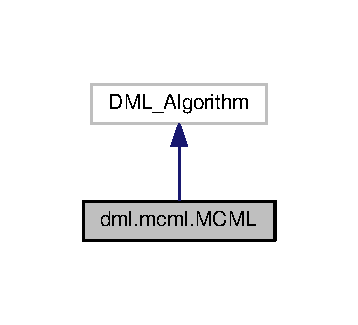
\includegraphics[width=172pt]{classdml_1_1mcml_1_1MCML__inherit__graph}
\end{center}
\end{figure}


Collaboration diagram for dml.\+mcml.\+M\+C\+ML\+:
\nopagebreak
\begin{figure}[H]
\begin{center}
\leavevmode
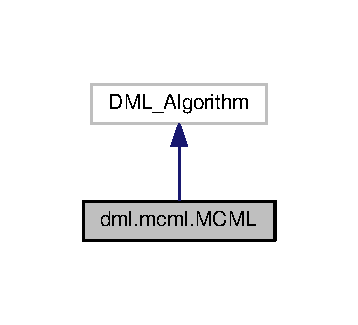
\includegraphics[width=172pt]{classdml_1_1mcml_1_1MCML__coll__graph}
\end{center}
\end{figure}
\subsection*{Public Member Functions}
\begin{DoxyCompactItemize}
\item 
def {\bfseries \+\_\+\+\_\+init\+\_\+\+\_\+} (self, num\+\_\+dims=None, learning\+\_\+rate=\char`\"{}adaptive\char`\"{}, eta0=0.\+01, initial\+\_\+metric=None, max\+\_\+iter=20, prec=0.\+01, tol=0.\+01, descent\+\_\+method=\char`\"{}S\+DP\char`\"{}, eta\+\_\+thres=1e-\/14, learn\+\_\+inc=1.\+01, learn\+\_\+dec=0.\+5)\hypertarget{classdml_1_1mcml_1_1MCML_ab24bfae43298806c065030a453dd6613}{}\label{classdml_1_1mcml_1_1MCML_ab24bfae43298806c065030a453dd6613}

\item 
def \hyperlink{classdml_1_1mcml_1_1MCML_a73bb7173d9688126b49e585ff4434892}{metadata} (self)
\item 
def \hyperlink{classdml_1_1mcml_1_1MCML_ad1980c9bf7c3b8843d36f8f1666e08a6}{metric} (self)
\item 
def \hyperlink{classdml_1_1mcml_1_1MCML_a0984330dd64aad712a46dcc3ba27baa8}{fit} (self, X, y)
\end{DoxyCompactItemize}
\subsection*{Public Attributes}
\begin{DoxyCompactItemize}
\item 
{\bfseries num\+\_\+dims\+\_\+}\hypertarget{classdml_1_1mcml_1_1MCML_adbb2311297903823e3af1c35086adb03}{}\label{classdml_1_1mcml_1_1MCML_adbb2311297903823e3af1c35086adb03}

\item 
{\bfseries initial\+\_\+}\hypertarget{classdml_1_1mcml_1_1MCML_ac05cdbdf44871053938723291e3bbee6}{}\label{classdml_1_1mcml_1_1MCML_ac05cdbdf44871053938723291e3bbee6}

\item 
{\bfseries max\+\_\+it\+\_\+}\hypertarget{classdml_1_1mcml_1_1MCML_ad952bdb80b531882c6b591761aa65543}{}\label{classdml_1_1mcml_1_1MCML_ad952bdb80b531882c6b591761aa65543}

\item 
{\bfseries eta\+\_\+}\hypertarget{classdml_1_1mcml_1_1MCML_aa2faa2f85ba20baae9fdcfdcb1b0fdaa}{}\label{classdml_1_1mcml_1_1MCML_aa2faa2f85ba20baae9fdcfdcb1b0fdaa}

\item 
{\bfseries eta0\+\_\+}\hypertarget{classdml_1_1mcml_1_1MCML_a8a5b6805251ee054de00f35aa9917dde}{}\label{classdml_1_1mcml_1_1MCML_a8a5b6805251ee054de00f35aa9917dde}

\item 
{\bfseries learning\+\_\+}\hypertarget{classdml_1_1mcml_1_1MCML_a7830eb3bf60dd1698419307a765fcb6e}{}\label{classdml_1_1mcml_1_1MCML_a7830eb3bf60dd1698419307a765fcb6e}

\item 
{\bfseries adaptive\+\_\+}\hypertarget{classdml_1_1mcml_1_1MCML_a7bb39b6f8b31b3006c84c9a43bbe70ea}{}\label{classdml_1_1mcml_1_1MCML_a7bb39b6f8b31b3006c84c9a43bbe70ea}

\item 
{\bfseries method\+\_\+}\hypertarget{classdml_1_1mcml_1_1MCML_a38f3cbfba1e4de7dce453816f9b7ab62}{}\label{classdml_1_1mcml_1_1MCML_a38f3cbfba1e4de7dce453816f9b7ab62}

\item 
{\bfseries eps\+\_\+}\hypertarget{classdml_1_1mcml_1_1MCML_a3e47e84c124eac05a5f110968d22b621}{}\label{classdml_1_1mcml_1_1MCML_a3e47e84c124eac05a5f110968d22b621}

\item 
{\bfseries tol\+\_\+}\hypertarget{classdml_1_1mcml_1_1MCML_ab5064a7c7e7214b17015aed86775f8a9}{}\label{classdml_1_1mcml_1_1MCML_ab5064a7c7e7214b17015aed86775f8a9}

\item 
{\bfseries etamin\+\_\+}\hypertarget{classdml_1_1mcml_1_1MCML_ae4f8ac49bc3fe3a7f49b18c6f56cba6a}{}\label{classdml_1_1mcml_1_1MCML_ae4f8ac49bc3fe3a7f49b18c6f56cba6a}

\item 
{\bfseries l\+\_\+inc\+\_\+}\hypertarget{classdml_1_1mcml_1_1MCML_aee3082de50ebefa808212a716346e760}{}\label{classdml_1_1mcml_1_1MCML_aee3082de50ebefa808212a716346e760}

\item 
{\bfseries l\+\_\+dec\+\_\+}\hypertarget{classdml_1_1mcml_1_1MCML_ab6510f4cb97eca6e4be9bad38c24a4fb}{}\label{classdml_1_1mcml_1_1MCML_ab6510f4cb97eca6e4be9bad38c24a4fb}

\item 
{\bfseries num\+\_\+its\+\_\+}\hypertarget{classdml_1_1mcml_1_1MCML_a00afb19f4afcc26aeb6e7367ef4564c4}{}\label{classdml_1_1mcml_1_1MCML_a00afb19f4afcc26aeb6e7367ef4564c4}

\item 
{\bfseries initial\+\_\+error\+\_\+}\hypertarget{classdml_1_1mcml_1_1MCML_a2243dbb87e3ba75ba0697f4d59bee713}{}\label{classdml_1_1mcml_1_1MCML_a2243dbb87e3ba75ba0697f4d59bee713}

\item 
{\bfseries final\+\_\+error\+\_\+}\hypertarget{classdml_1_1mcml_1_1MCML_aa63de6f27a2ff66305e05ab96c5d4abd}{}\label{classdml_1_1mcml_1_1MCML_aa63de6f27a2ff66305e05ab96c5d4abd}

\item 
{\bfseries d\+\_\+}\hypertarget{classdml_1_1mcml_1_1MCML_a5cf1cb67a506cf18026feb7e8ed3ad0f}{}\label{classdml_1_1mcml_1_1MCML_a5cf1cb67a506cf18026feb7e8ed3ad0f}

\item 
{\bfseries nd\+\_\+}\hypertarget{classdml_1_1mcml_1_1MCML_a122dd4093562f818ccbeae30a6688641}{}\label{classdml_1_1mcml_1_1MCML_a122dd4093562f818ccbeae30a6688641}

\item 
{\bfseries X\+\_\+}\hypertarget{classdml_1_1mcml_1_1MCML_ad8dfded232cd94061f0c9bc79f3ff853}{}\label{classdml_1_1mcml_1_1MCML_ad8dfded232cd94061f0c9bc79f3ff853}

\item 
{\bfseries y\+\_\+}\hypertarget{classdml_1_1mcml_1_1MCML_acb9ba109473371b373773ec00b43f0e6}{}\label{classdml_1_1mcml_1_1MCML_acb9ba109473371b373773ec00b43f0e6}

\item 
{\bfseries M\+\_\+}\hypertarget{classdml_1_1mcml_1_1MCML_a783cb7d5548a0bff784d8309cbf6ac15}{}\label{classdml_1_1mcml_1_1MCML_a783cb7d5548a0bff784d8309cbf6ac15}

\end{DoxyCompactItemize}


\subsection{Detailed Description}
\begin{DoxyVerb}Maximally Collapsing Metric Learning (MCML)

A distance metric learning algorithm that learns minimizing the KL divergence to the maximally collapsing distribution.

Parameters
----------

num_dims : int, default=None.

    Number of dimensions for dimensionality reduction. Not supported yet.

learning_rate : string, default='adaptive'

    Type of learning rate update for gradient descent. Possible values are:

    - 'adaptive' : the learning rate will increase if the gradient step is succesful, else it will decrease.

    - 'constant' : the learning rate will be constant during all the gradient steps.

eta0 : float, default=0.01

    The initial value for learning rate.

initial_metric : 2D-Array or Matrix (d x d), or string, default=None.

    If array or matrix, it must be a positive semidefinite matrix with the starting metric for gradient descent, where d is the number of features.
    If None, euclidean distance will be used. If a string, the following values are allowed:

    - 'euclidean' : the euclidean distance.

    - 'scale' : a diagonal matrix that normalizes each attribute according to its range will be used.

max_iter : int, default=20

    Maximum number of iterations of gradient descent.

prec : float, default=1e-3

    Precision stop criterion (gradient norm).

tol : float, default=1e-3

    Tolerance stop criterion (difference between two iterations)

descent_method : string, default='SDP'

    The descent method to use. Allowed values are:

    - 'SDP' : semidefinite programming, consisting of gradient descent with projections onto the PSD cone.

eta_thres : float, default=1e-14

    A learning rate threshold stop criterion.

learn_inc : float, default=1.01

    Increase factor for learning rate. Ignored if learning_rate is not 'adaptive'.

learn_dec : float, default=0.5

    Decrease factor for learning rate. Ignored if learning_rate is not 'adaptive'.

References
----------
    Amir Globerson and Sam T Roweis. “Metric learning by collapsing classes”. In: Advances in neural
    information processing systems. 2006, pages 451-458.
\end{DoxyVerb}
 

\subsection{Member Function Documentation}
\index{dml\+::mcml\+::\+M\+C\+ML@{dml\+::mcml\+::\+M\+C\+ML}!fit@{fit}}
\index{fit@{fit}!dml\+::mcml\+::\+M\+C\+ML@{dml\+::mcml\+::\+M\+C\+ML}}
\subsubsection[{\texorpdfstring{fit(self, X, y)}{fit(self, X, y)}}]{\setlength{\rightskip}{0pt plus 5cm}def dml.\+mcml.\+M\+C\+M\+L.\+fit (
\begin{DoxyParamCaption}
\item[{}]{self, }
\item[{}]{X, }
\item[{}]{y}
\end{DoxyParamCaption}
)}\hypertarget{classdml_1_1mcml_1_1MCML_a0984330dd64aad712a46dcc3ba27baa8}{}\label{classdml_1_1mcml_1_1MCML_a0984330dd64aad712a46dcc3ba27baa8}
\begin{DoxyVerb}Fit the model from the data in X and the labels in y.

Parameters
----------
X : array-like, shape (N x d)
    Training vector, where N is the number of samples, and d is the number of features.

y : array-like, shape (N)
    Labels vector, where N is the number of samples.

Returns
-------
self : object
    Returns the instance itself.
\end{DoxyVerb}
 \index{dml\+::mcml\+::\+M\+C\+ML@{dml\+::mcml\+::\+M\+C\+ML}!metadata@{metadata}}
\index{metadata@{metadata}!dml\+::mcml\+::\+M\+C\+ML@{dml\+::mcml\+::\+M\+C\+ML}}
\subsubsection[{\texorpdfstring{metadata(self)}{metadata(self)}}]{\setlength{\rightskip}{0pt plus 5cm}def dml.\+mcml.\+M\+C\+M\+L.\+metadata (
\begin{DoxyParamCaption}
\item[{}]{self}
\end{DoxyParamCaption}
)}\hypertarget{classdml_1_1mcml_1_1MCML_a73bb7173d9688126b49e585ff4434892}{}\label{classdml_1_1mcml_1_1MCML_a73bb7173d9688126b49e585ff4434892}
\begin{DoxyVerb}Obtains algorithm metadata.

Returns
-------
meta : A dictionary with the following metadata:
    - 'num_iters' : Number of iterations that the descent method took.

    - 'initial_error' : Initial value of the objective function.

    - 'final_error' : Final value of the objective function.
\end{DoxyVerb}
 \index{dml\+::mcml\+::\+M\+C\+ML@{dml\+::mcml\+::\+M\+C\+ML}!metric@{metric}}
\index{metric@{metric}!dml\+::mcml\+::\+M\+C\+ML@{dml\+::mcml\+::\+M\+C\+ML}}
\subsubsection[{\texorpdfstring{metric(self)}{metric(self)}}]{\setlength{\rightskip}{0pt plus 5cm}def dml.\+mcml.\+M\+C\+M\+L.\+metric (
\begin{DoxyParamCaption}
\item[{}]{self}
\end{DoxyParamCaption}
)}\hypertarget{classdml_1_1mcml_1_1MCML_ad1980c9bf7c3b8843d36f8f1666e08a6}{}\label{classdml_1_1mcml_1_1MCML_ad1980c9bf7c3b8843d36f8f1666e08a6}
\begin{DoxyVerb}Obtains the learned metric.

Returns
-------
M : (dxd) positive semidefinite matrix, where d is the number of features.
\end{DoxyVerb}
 

The documentation for this class was generated from the following file\+:\begin{DoxyCompactItemize}
\item 
dml/mcml.\+pyx\end{DoxyCompactItemize}

\hypertarget{classdml_1_1base_1_1Metric}{}\section{dml.\+base.\+Metric Class Reference}
\label{classdml_1_1base_1_1Metric}\index{dml.\+base.\+Metric@{dml.\+base.\+Metric}}


Inheritance diagram for dml.\+base.\+Metric\+:\nopagebreak
\begin{figure}[H]
\begin{center}
\leavevmode
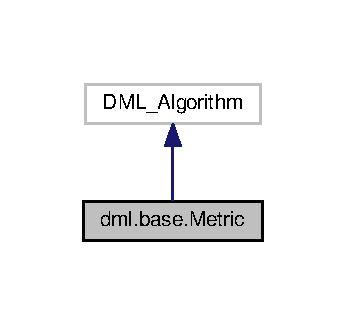
\includegraphics[width=166pt]{classdml_1_1base_1_1Metric__inherit__graph}
\end{center}
\end{figure}


Collaboration diagram for dml.\+base.\+Metric\+:\nopagebreak
\begin{figure}[H]
\begin{center}
\leavevmode
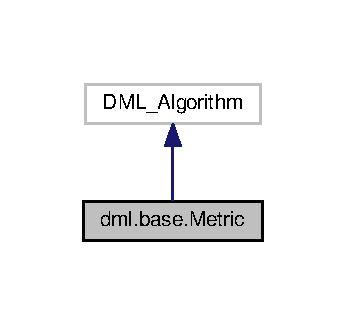
\includegraphics[width=166pt]{classdml_1_1base_1_1Metric__coll__graph}
\end{center}
\end{figure}
\subsection*{Public Member Functions}
\begin{DoxyCompactItemize}
\item 
def {\bfseries \+\_\+\+\_\+init\+\_\+\+\_\+} (self, \hyperlink{classdml_1_1base_1_1Metric_a41a9f7544ff22d3b05e3b5451e4c16b0}{metric})\hypertarget{classdml_1_1base_1_1Metric_aca79aaafeef1b4b94081a24579f2f254}{}\label{classdml_1_1base_1_1Metric_aca79aaafeef1b4b94081a24579f2f254}

\item 
def \hyperlink{classdml_1_1base_1_1Metric_ad94ffd257c24ae5e291d301131bbd874}{fit} (self, X, y)
\item 
def \hyperlink{classdml_1_1base_1_1Metric_a41a9f7544ff22d3b05e3b5451e4c16b0}{metric} (self)
\end{DoxyCompactItemize}
\subsection*{Public Attributes}
\begin{DoxyCompactItemize}
\item 
{\bfseries M\+\_\+}\hypertarget{classdml_1_1base_1_1Metric_a85246f8f52ee2c28c077e435c2699fe1}{}\label{classdml_1_1base_1_1Metric_a85246f8f52ee2c28c077e435c2699fe1}

\item 
{\bfseries y\+\_\+}\hypertarget{classdml_1_1base_1_1Metric_ad333d6abb88aabb0d0532cb31a56cf32}{}\label{classdml_1_1base_1_1Metric_ad333d6abb88aabb0d0532cb31a56cf32}

\end{DoxyCompactItemize}


\subsection{Detailed Description}
\begin{DoxyVerb}A DML algorithm that defines a distance given a PSD metric matrix.

Parameters
----------

metric : (d x d) matrix. A positive semidefinite matrix, to define a pseudodistance in euclidean d-dimensional space.
\end{DoxyVerb}
 

\subsection{Member Function Documentation}
\index{dml\+::base\+::\+Metric@{dml\+::base\+::\+Metric}!fit@{fit}}
\index{fit@{fit}!dml\+::base\+::\+Metric@{dml\+::base\+::\+Metric}}
\subsubsection[{\texorpdfstring{fit(self, X, y)}{fit(self, X, y)}}]{\setlength{\rightskip}{0pt plus 5cm}def dml.\+base.\+Metric.\+fit (
\begin{DoxyParamCaption}
\item[{}]{self, }
\item[{}]{X, }
\item[{}]{y}
\end{DoxyParamCaption}
)}\hypertarget{classdml_1_1base_1_1Metric_ad94ffd257c24ae5e291d301131bbd874}{}\label{classdml_1_1base_1_1Metric_ad94ffd257c24ae5e291d301131bbd874}
\begin{DoxyVerb}Fit the model from the data in X and the labels in y.

Parameters
----------
X : array-like, shape (N x d)
    Training vector, where N is the number of samples, and d is the number of features.

y : array-like, shape (N)
    Labels vector, where N is the number of samples.

Returns
-------
self : object
    Returns the instance itself.
\end{DoxyVerb}
 \index{dml\+::base\+::\+Metric@{dml\+::base\+::\+Metric}!metric@{metric}}
\index{metric@{metric}!dml\+::base\+::\+Metric@{dml\+::base\+::\+Metric}}
\subsubsection[{\texorpdfstring{metric(self)}{metric(self)}}]{\setlength{\rightskip}{0pt plus 5cm}def dml.\+base.\+Metric.\+metric (
\begin{DoxyParamCaption}
\item[{}]{self}
\end{DoxyParamCaption}
)}\hypertarget{classdml_1_1base_1_1Metric_a41a9f7544ff22d3b05e3b5451e4c16b0}{}\label{classdml_1_1base_1_1Metric_a41a9f7544ff22d3b05e3b5451e4c16b0}
\begin{DoxyVerb}Obtains the learned metric.

Returns
-------
M : (dxd) positive semidefinite matrix, where d is the number of features.
\end{DoxyVerb}
 

The documentation for this class was generated from the following file\+:\begin{DoxyCompactItemize}
\item 
dml/base.\+py\end{DoxyCompactItemize}

\hypertarget{classdml_1_1multidml__knn_1_1MultiDML__kNN}{}\section{dml.\+multidml\+\_\+knn.\+Multi\+D\+M\+L\+\_\+k\+NN Class Reference}
\label{classdml_1_1multidml__knn_1_1MultiDML__kNN}\index{dml.\+multidml\+\_\+knn.\+Multi\+D\+M\+L\+\_\+k\+NN@{dml.\+multidml\+\_\+knn.\+Multi\+D\+M\+L\+\_\+k\+NN}}
\subsection*{Public Member Functions}
\begin{DoxyCompactItemize}
\item 
def {\bfseries \+\_\+\+\_\+init\+\_\+\+\_\+} (self, n\+\_\+neighbors, dmls=None, verbose=False, knn\+\_\+args)\hypertarget{classdml_1_1multidml__knn_1_1MultiDML__kNN_a8539a84676b0b9a554797907b5238069}{}\label{classdml_1_1multidml__knn_1_1MultiDML__kNN_a8539a84676b0b9a554797907b5238069}

\item 
def \hyperlink{classdml_1_1multidml__knn_1_1MultiDML__kNN_a7b980f08da2a002708a7f753a4d07dda}{add} (self, dmls)
\item 
def \hyperlink{classdml_1_1multidml__knn_1_1MultiDML__kNN_a75eeeb787411f911f203ad06ed4c5764}{fit} (self, X, y)
\item 
def \hyperlink{classdml_1_1multidml__knn_1_1MultiDML__kNN_a351feb6aca364a137f8f816cc781ac50}{elapsed} (self)
\item 
def \hyperlink{classdml_1_1multidml__knn_1_1MultiDML__kNN_aa0dcf8938bcddba60f78f63d3314a716}{predict\+\_\+all} (self, X=None)
\item 
def \hyperlink{classdml_1_1multidml__knn_1_1MultiDML__kNN_a623e8af8fb11433d6cb3627e29928d2e}{predict\+\_\+proba\+\_\+all} (self, X=None)
\item 
def \hyperlink{classdml_1_1multidml__knn_1_1MultiDML__kNN_a8f8fcc90ff495bbb5f4f52636244d1aa}{score\+\_\+all} (self, X=None, y=None)
\item 
def \hyperlink{classdml_1_1multidml__knn_1_1MultiDML__kNN_ac475b5d23239fdf0823fe2e4e25c6723}{dmls\+\_\+string} (self)
\end{DoxyCompactItemize}
\subsection*{Public Attributes}
\begin{DoxyCompactItemize}
\item 
{\bfseries nn\+\_\+}\hypertarget{classdml_1_1multidml__knn_1_1MultiDML__kNN_a158ad1c37eb32c2aa22c09ae483e3b18}{}\label{classdml_1_1multidml__knn_1_1MultiDML__kNN_a158ad1c37eb32c2aa22c09ae483e3b18}

\item 
{\bfseries knn\+\_\+args\+\_\+}\hypertarget{classdml_1_1multidml__knn_1_1MultiDML__kNN_a116c9aaf6af321024ab915c0766e85fe}{}\label{classdml_1_1multidml__knn_1_1MultiDML__kNN_a116c9aaf6af321024ab915c0766e85fe}

\item 
{\bfseries knns\+\_\+}\hypertarget{classdml_1_1multidml__knn_1_1MultiDML__kNN_a114a09af63f5c23ae99da995c605e342}{}\label{classdml_1_1multidml__knn_1_1MultiDML__kNN_a114a09af63f5c23ae99da995c605e342}

\item 
{\bfseries verbose\+\_\+}\hypertarget{classdml_1_1multidml__knn_1_1MultiDML__kNN_a2c5a6599aab8dd18a871ef32d8cddab4}{}\label{classdml_1_1multidml__knn_1_1MultiDML__kNN_a2c5a6599aab8dd18a871ef32d8cddab4}

\item 
{\bfseries dmls\+\_\+}\hypertarget{classdml_1_1multidml__knn_1_1MultiDML__kNN_aa1c964de12668befb05c3c921ab159c7}{}\label{classdml_1_1multidml__knn_1_1MultiDML__kNN_aa1c964de12668befb05c3c921ab159c7}

\item 
{\bfseries X\+\_\+}\hypertarget{classdml_1_1multidml__knn_1_1MultiDML__kNN_a73e34e73fff5af366187066039030b40}{}\label{classdml_1_1multidml__knn_1_1MultiDML__kNN_a73e34e73fff5af366187066039030b40}

\item 
{\bfseries y\+\_\+}\hypertarget{classdml_1_1multidml__knn_1_1MultiDML__kNN_a131e523cff5282a04e085f7f92b6c715}{}\label{classdml_1_1multidml__knn_1_1MultiDML__kNN_a131e523cff5282a04e085f7f92b6c715}

\item 
{\bfseries num\+\_\+labels\+\_\+}\hypertarget{classdml_1_1multidml__knn_1_1MultiDML__kNN_a736bd03da045ff53a2ac23d4217e76cc}{}\label{classdml_1_1multidml__knn_1_1MultiDML__kNN_a736bd03da045ff53a2ac23d4217e76cc}

\item 
{\bfseries elapsed\+\_\+}\hypertarget{classdml_1_1multidml__knn_1_1MultiDML__kNN_a7b9ad174e9bc04ffa0b1393cec489f0b}{}\label{classdml_1_1multidml__knn_1_1MultiDML__kNN_a7b9ad174e9bc04ffa0b1393cec489f0b}

\end{DoxyCompactItemize}


\subsection{Detailed Description}
\begin{DoxyVerb}Multi-DML k-NN

An interface that allows learning k-NN with different distance metric learners simultaneously.

Parameters
----------

n_neighbors : int

    The number of neighbors for k-NN.

dmls : list, default=None

    A list of distance metric learning algorithms to be learned for k-NN. By default, euclidean distance will be added at the first
    place of the dml list.

verbose : boolean, default=False

    If True, console message about the algorithms execution will be printed.\end{DoxyVerb}
 

\subsection{Member Function Documentation}
\index{dml\+::multidml\+\_\+knn\+::\+Multi\+D\+M\+L\+\_\+k\+NN@{dml\+::multidml\+\_\+knn\+::\+Multi\+D\+M\+L\+\_\+k\+NN}!add@{add}}
\index{add@{add}!dml\+::multidml\+\_\+knn\+::\+Multi\+D\+M\+L\+\_\+k\+NN@{dml\+::multidml\+\_\+knn\+::\+Multi\+D\+M\+L\+\_\+k\+NN}}
\subsubsection[{\texorpdfstring{add(self, dmls)}{add(self, dmls)}}]{\setlength{\rightskip}{0pt plus 5cm}def dml.\+multidml\+\_\+knn.\+Multi\+D\+M\+L\+\_\+k\+N\+N.\+add (
\begin{DoxyParamCaption}
\item[{}]{self, }
\item[{}]{dmls}
\end{DoxyParamCaption}
)}\hypertarget{classdml_1_1multidml__knn_1_1MultiDML__kNN_a7b980f08da2a002708a7f753a4d07dda}{}\label{classdml_1_1multidml__knn_1_1MultiDML__kNN_a7b980f08da2a002708a7f753a4d07dda}
\begin{DoxyVerb}Adds a new distance metric learning algorithm to the list.

Parameters
----------

dmls : DML_Algorithm, or list of DMÑ_Algorithm

    The DML algorithm or algorithms to add.\end{DoxyVerb}
 \index{dml\+::multidml\+\_\+knn\+::\+Multi\+D\+M\+L\+\_\+k\+NN@{dml\+::multidml\+\_\+knn\+::\+Multi\+D\+M\+L\+\_\+k\+NN}!dmls\+\_\+string@{dmls\+\_\+string}}
\index{dmls\+\_\+string@{dmls\+\_\+string}!dml\+::multidml\+\_\+knn\+::\+Multi\+D\+M\+L\+\_\+k\+NN@{dml\+::multidml\+\_\+knn\+::\+Multi\+D\+M\+L\+\_\+k\+NN}}
\subsubsection[{\texorpdfstring{dmls\+\_\+string(self)}{dmls_string(self)}}]{\setlength{\rightskip}{0pt plus 5cm}def dml.\+multidml\+\_\+knn.\+Multi\+D\+M\+L\+\_\+k\+N\+N.\+dmls\+\_\+string (
\begin{DoxyParamCaption}
\item[{}]{self}
\end{DoxyParamCaption}
)}\hypertarget{classdml_1_1multidml__knn_1_1MultiDML__kNN_ac475b5d23239fdf0823fe2e4e25c6723}{}\label{classdml_1_1multidml__knn_1_1MultiDML__kNN_ac475b5d23239fdf0823fe2e4e25c6723}
\begin{DoxyVerb}Obtains the strings with the dml names.

Returns
-------

strings : A list with the names of each dml.
\end{DoxyVerb}
 \index{dml\+::multidml\+\_\+knn\+::\+Multi\+D\+M\+L\+\_\+k\+NN@{dml\+::multidml\+\_\+knn\+::\+Multi\+D\+M\+L\+\_\+k\+NN}!elapsed@{elapsed}}
\index{elapsed@{elapsed}!dml\+::multidml\+\_\+knn\+::\+Multi\+D\+M\+L\+\_\+k\+NN@{dml\+::multidml\+\_\+knn\+::\+Multi\+D\+M\+L\+\_\+k\+NN}}
\subsubsection[{\texorpdfstring{elapsed(self)}{elapsed(self)}}]{\setlength{\rightskip}{0pt plus 5cm}def dml.\+multidml\+\_\+knn.\+Multi\+D\+M\+L\+\_\+k\+N\+N.\+elapsed (
\begin{DoxyParamCaption}
\item[{}]{self}
\end{DoxyParamCaption}
)}\hypertarget{classdml_1_1multidml__knn_1_1MultiDML__kNN_a351feb6aca364a137f8f816cc781ac50}{}\label{classdml_1_1multidml__knn_1_1MultiDML__kNN_a351feb6aca364a137f8f816cc781ac50}
\begin{DoxyVerb}Obtains the elapsed time of each DML algorithm

Returns
-------

elapsed : A list of float with the time of each DML.
\end{DoxyVerb}
 \index{dml\+::multidml\+\_\+knn\+::\+Multi\+D\+M\+L\+\_\+k\+NN@{dml\+::multidml\+\_\+knn\+::\+Multi\+D\+M\+L\+\_\+k\+NN}!fit@{fit}}
\index{fit@{fit}!dml\+::multidml\+\_\+knn\+::\+Multi\+D\+M\+L\+\_\+k\+NN@{dml\+::multidml\+\_\+knn\+::\+Multi\+D\+M\+L\+\_\+k\+NN}}
\subsubsection[{\texorpdfstring{fit(self, X, y)}{fit(self, X, y)}}]{\setlength{\rightskip}{0pt plus 5cm}def dml.\+multidml\+\_\+knn.\+Multi\+D\+M\+L\+\_\+k\+N\+N.\+fit (
\begin{DoxyParamCaption}
\item[{}]{self, }
\item[{}]{X, }
\item[{}]{y}
\end{DoxyParamCaption}
)}\hypertarget{classdml_1_1multidml__knn_1_1MultiDML__kNN_a75eeeb787411f911f203ad06ed4c5764}{}\label{classdml_1_1multidml__knn_1_1MultiDML__kNN_a75eeeb787411f911f203ad06ed4c5764}
\begin{DoxyVerb}Fit the model from the data in X and the labels in y.

Parameters
----------
X : array-like, shape (N x d)
    Training vector, where N is the number of samples, and d is the number of features.

y : array-like, shape (N)
    Labels vector, where N is the number of samples.

Returns
-------
self : object
    Returns the instance itself.
\end{DoxyVerb}
 \index{dml\+::multidml\+\_\+knn\+::\+Multi\+D\+M\+L\+\_\+k\+NN@{dml\+::multidml\+\_\+knn\+::\+Multi\+D\+M\+L\+\_\+k\+NN}!predict\+\_\+all@{predict\+\_\+all}}
\index{predict\+\_\+all@{predict\+\_\+all}!dml\+::multidml\+\_\+knn\+::\+Multi\+D\+M\+L\+\_\+k\+NN@{dml\+::multidml\+\_\+knn\+::\+Multi\+D\+M\+L\+\_\+k\+NN}}
\subsubsection[{\texorpdfstring{predict\+\_\+all(self, X=\+None)}{predict_all(self, X=None)}}]{\setlength{\rightskip}{0pt plus 5cm}def dml.\+multidml\+\_\+knn.\+Multi\+D\+M\+L\+\_\+k\+N\+N.\+predict\+\_\+all (
\begin{DoxyParamCaption}
\item[{}]{self, }
\item[{}]{X = {\ttfamily None}}
\end{DoxyParamCaption}
)}\hypertarget{classdml_1_1multidml__knn_1_1MultiDML__kNN_aa0dcf8938bcddba60f78f63d3314a716}{}\label{classdml_1_1multidml__knn_1_1MultiDML__kNN_aa0dcf8938bcddba60f78f63d3314a716}
\begin{DoxyVerb}Predicts the labels for the given data. Model needs to be already fitted.

X : 2D-Array or Matrix, default=None

    The dataset to be used. If None, the training set will be used. In this case, the prediction will be made
    using Leave One Out (that is, the sample to predict will be taken away from the training set).

Returns
-------

y : list of 1D-Arrays

    A list with the vectors with the label predictions for each DML.
\end{DoxyVerb}
 \index{dml\+::multidml\+\_\+knn\+::\+Multi\+D\+M\+L\+\_\+k\+NN@{dml\+::multidml\+\_\+knn\+::\+Multi\+D\+M\+L\+\_\+k\+NN}!predict\+\_\+proba\+\_\+all@{predict\+\_\+proba\+\_\+all}}
\index{predict\+\_\+proba\+\_\+all@{predict\+\_\+proba\+\_\+all}!dml\+::multidml\+\_\+knn\+::\+Multi\+D\+M\+L\+\_\+k\+NN@{dml\+::multidml\+\_\+knn\+::\+Multi\+D\+M\+L\+\_\+k\+NN}}
\subsubsection[{\texorpdfstring{predict\+\_\+proba\+\_\+all(self, X=\+None)}{predict_proba_all(self, X=None)}}]{\setlength{\rightskip}{0pt plus 5cm}def dml.\+multidml\+\_\+knn.\+Multi\+D\+M\+L\+\_\+k\+N\+N.\+predict\+\_\+proba\+\_\+all (
\begin{DoxyParamCaption}
\item[{}]{self, }
\item[{}]{X = {\ttfamily None}}
\end{DoxyParamCaption}
)}\hypertarget{classdml_1_1multidml__knn_1_1MultiDML__kNN_a623e8af8fb11433d6cb3627e29928d2e}{}\label{classdml_1_1multidml__knn_1_1MultiDML__kNN_a623e8af8fb11433d6cb3627e29928d2e}
\begin{DoxyVerb}Predicts the probabilities for the given data. Model needs to be already fitted.

X : 2D-Array or Matrix, default=None

    The dataset to be used. If None, the training set will be used. In this case, the prediction will be made
    using Leave One Out (that is, the sample to predict will be taken away from the training set).

Returns
-------

T : list of 2D-Arrays

    A list with the matrices with the label probabilities for each class, for each DML.
\end{DoxyVerb}
 \index{dml\+::multidml\+\_\+knn\+::\+Multi\+D\+M\+L\+\_\+k\+NN@{dml\+::multidml\+\_\+knn\+::\+Multi\+D\+M\+L\+\_\+k\+NN}!score\+\_\+all@{score\+\_\+all}}
\index{score\+\_\+all@{score\+\_\+all}!dml\+::multidml\+\_\+knn\+::\+Multi\+D\+M\+L\+\_\+k\+NN@{dml\+::multidml\+\_\+knn\+::\+Multi\+D\+M\+L\+\_\+k\+NN}}
\subsubsection[{\texorpdfstring{score\+\_\+all(self, X=\+None, y=\+None)}{score_all(self, X=None, y=None)}}]{\setlength{\rightskip}{0pt plus 5cm}def dml.\+multidml\+\_\+knn.\+Multi\+D\+M\+L\+\_\+k\+N\+N.\+score\+\_\+all (
\begin{DoxyParamCaption}
\item[{}]{self, }
\item[{}]{X = {\ttfamily None}, }
\item[{}]{y = {\ttfamily None}}
\end{DoxyParamCaption}
)}\hypertarget{classdml_1_1multidml__knn_1_1MultiDML__kNN_a8f8fcc90ff495bbb5f4f52636244d1aa}{}\label{classdml_1_1multidml__knn_1_1MultiDML__kNN_a8f8fcc90ff495bbb5f4f52636244d1aa}
\begin{DoxyVerb}Obtains the scores for the given data. Model needs to be already fitted.

X : 2D-Array or Matrix, default=None

    The dataset to be used. If None, the training set will be used. In this case, the prediction will be made
    using Leave One Out (that is, the sample to predict will be taken away from the training set).

Returns
-------

s : list of float

    A list with the k-NN scores for each DML.
\end{DoxyVerb}
 

The documentation for this class was generated from the following file\+:\begin{DoxyCompactItemize}
\item 
dml/multidml\+\_\+knn.\+py\end{DoxyCompactItemize}

\hypertarget{classdml_1_1nca_1_1NCA}{}\section{dml.\+nca.\+N\+CA Class Reference}
\label{classdml_1_1nca_1_1NCA}\index{dml.\+nca.\+N\+CA@{dml.\+nca.\+N\+CA}}


Inheritance diagram for dml.\+nca.\+N\+CA\+:
\nopagebreak
\begin{figure}[H]
\begin{center}
\leavevmode
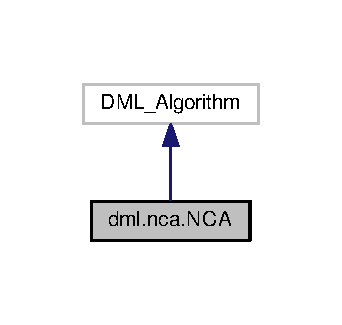
\includegraphics[width=164pt]{classdml_1_1nca_1_1NCA__inherit__graph}
\end{center}
\end{figure}


Collaboration diagram for dml.\+nca.\+N\+CA\+:
\nopagebreak
\begin{figure}[H]
\begin{center}
\leavevmode
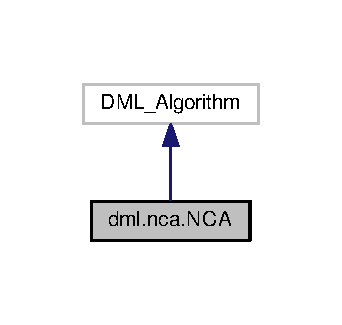
\includegraphics[width=164pt]{classdml_1_1nca_1_1NCA__coll__graph}
\end{center}
\end{figure}
\subsection*{Public Member Functions}
\begin{DoxyCompactItemize}
\item 
def {\bfseries \+\_\+\+\_\+init\+\_\+\+\_\+} (self, num\+\_\+dims=None, learning\+\_\+rate=\char`\"{}adaptive\char`\"{}, eta0=0.\+3, initial\+\_\+transform=None, max\+\_\+iter=100, prec=1e-\/8, tol=1e-\/8, descent\+\_\+method=\char`\"{}\+S\+G\+D\char`\"{}, eta\+\_\+thres=1e-\/14, learn\+\_\+inc=1.\+01, learn\+\_\+dec=0.\+5)\hypertarget{classdml_1_1nca_1_1NCA_a86bb8dcbd925eb0be6479ab0e0d3fb22}{}\label{classdml_1_1nca_1_1NCA_a86bb8dcbd925eb0be6479ab0e0d3fb22}

\item 
def \hyperlink{classdml_1_1nca_1_1NCA_adb91f357b09c4c4188c6425a537b9330}{metadata} (self)
\item 
def \hyperlink{classdml_1_1nca_1_1NCA_a5d302fa9ea28b6857f3f9b2b7efb7c99}{transformer} (self)
\item 
def \hyperlink{classdml_1_1nca_1_1NCA_af8a6f753d4d4cc1b49d6dfdb8b44d73a}{fit} (self, X, y)
\end{DoxyCompactItemize}
\subsection*{Public Attributes}
\begin{DoxyCompactItemize}
\item 
{\bfseries num\+\_\+dims\+\_\+}\hypertarget{classdml_1_1nca_1_1NCA_aae858f8447f17e1b9b2358084ba210ed}{}\label{classdml_1_1nca_1_1NCA_aae858f8447f17e1b9b2358084ba210ed}

\item 
{\bfseries L0\+\_\+}\hypertarget{classdml_1_1nca_1_1NCA_a01876307676c03a085fac3759aadaccc}{}\label{classdml_1_1nca_1_1NCA_a01876307676c03a085fac3759aadaccc}

\item 
{\bfseries max\+\_\+it\+\_\+}\hypertarget{classdml_1_1nca_1_1NCA_a19accf1175911523f947f66865fdc79c}{}\label{classdml_1_1nca_1_1NCA_a19accf1175911523f947f66865fdc79c}

\item 
{\bfseries eta\+\_\+}\hypertarget{classdml_1_1nca_1_1NCA_ad005ff4569cf5db0bcb55349adf8dc55}{}\label{classdml_1_1nca_1_1NCA_ad005ff4569cf5db0bcb55349adf8dc55}

\item 
{\bfseries eta0\+\_\+}\hypertarget{classdml_1_1nca_1_1NCA_af8f01006660da5d2e1e485163c21bd79}{}\label{classdml_1_1nca_1_1NCA_af8f01006660da5d2e1e485163c21bd79}

\item 
{\bfseries learning\+\_\+}\hypertarget{classdml_1_1nca_1_1NCA_af60d4fcb14a2703e266354034e96f7f0}{}\label{classdml_1_1nca_1_1NCA_af60d4fcb14a2703e266354034e96f7f0}

\item 
{\bfseries adaptive\+\_\+}\hypertarget{classdml_1_1nca_1_1NCA_aaa43fbc972c4ffcec4dc237337be38f0}{}\label{classdml_1_1nca_1_1NCA_aaa43fbc972c4ffcec4dc237337be38f0}

\item 
{\bfseries method\+\_\+}\hypertarget{classdml_1_1nca_1_1NCA_ad0113eb881f8529f05912c32a2f812a5}{}\label{classdml_1_1nca_1_1NCA_ad0113eb881f8529f05912c32a2f812a5}

\item 
{\bfseries eps\+\_\+}\hypertarget{classdml_1_1nca_1_1NCA_a62371155e2dc181c86c2029baca9a79f}{}\label{classdml_1_1nca_1_1NCA_a62371155e2dc181c86c2029baca9a79f}

\item 
{\bfseries tol\+\_\+}\hypertarget{classdml_1_1nca_1_1NCA_aed6186e6e52a5a8ee5b9d702e81323e3}{}\label{classdml_1_1nca_1_1NCA_aed6186e6e52a5a8ee5b9d702e81323e3}

\item 
{\bfseries etamin\+\_\+}\hypertarget{classdml_1_1nca_1_1NCA_ab6bf53dc847d68bb3ade5a62ac9c9a2b}{}\label{classdml_1_1nca_1_1NCA_ab6bf53dc847d68bb3ade5a62ac9c9a2b}

\item 
{\bfseries l\+\_\+inc\+\_\+}\hypertarget{classdml_1_1nca_1_1NCA_a48a1afdf5fa216d1920c9702220fbf44}{}\label{classdml_1_1nca_1_1NCA_a48a1afdf5fa216d1920c9702220fbf44}

\item 
{\bfseries l\+\_\+dec\+\_\+}\hypertarget{classdml_1_1nca_1_1NCA_ac9cb622f0a26c6287fb2c7c8f04211d5}{}\label{classdml_1_1nca_1_1NCA_ac9cb622f0a26c6287fb2c7c8f04211d5}

\item 
{\bfseries num\+\_\+its\+\_\+}\hypertarget{classdml_1_1nca_1_1NCA_a82a4d8e96d969702b6502fc1a55e290d}{}\label{classdml_1_1nca_1_1NCA_a82a4d8e96d969702b6502fc1a55e290d}

\item 
{\bfseries initial\+\_\+softmax\+\_\+}\hypertarget{classdml_1_1nca_1_1NCA_a59666362ce20353bd94d2458139b0698}{}\label{classdml_1_1nca_1_1NCA_a59666362ce20353bd94d2458139b0698}

\item 
{\bfseries final\+\_\+softmax\+\_\+}\hypertarget{classdml_1_1nca_1_1NCA_aa3c03274f76ee022048fc72380c2a375}{}\label{classdml_1_1nca_1_1NCA_aa3c03274f76ee022048fc72380c2a375}

\item 
{\bfseries d\+\_\+}\hypertarget{classdml_1_1nca_1_1NCA_a930059b9f0a023df96d65663bc2cdaa1}{}\label{classdml_1_1nca_1_1NCA_a930059b9f0a023df96d65663bc2cdaa1}

\item 
{\bfseries nd\+\_\+}\hypertarget{classdml_1_1nca_1_1NCA_aec8aad31b2c340c395e6cf2a6ef4050b}{}\label{classdml_1_1nca_1_1NCA_aec8aad31b2c340c395e6cf2a6ef4050b}

\item 
{\bfseries L\+\_\+}\hypertarget{classdml_1_1nca_1_1NCA_adc8c407795b11915d6a8ed4131ce22d0}{}\label{classdml_1_1nca_1_1NCA_adc8c407795b11915d6a8ed4131ce22d0}

\item 
{\bfseries X\+\_\+}\hypertarget{classdml_1_1nca_1_1NCA_a92379ea16856823e168e45eafda2f9ef}{}\label{classdml_1_1nca_1_1NCA_a92379ea16856823e168e45eafda2f9ef}

\item 
{\bfseries y\+\_\+}\hypertarget{classdml_1_1nca_1_1NCA_adb49c3d9bfa0aafc6ed6c4ed7adcfe96}{}\label{classdml_1_1nca_1_1NCA_adb49c3d9bfa0aafc6ed6c4ed7adcfe96}

\end{DoxyCompactItemize}


\subsection{Detailed Description}
\begin{DoxyVerb}Neighborhood Component Analysis (NCA)

A distance metric learning algorithm that tries to minimize kNN expected error.

Parameters
----------

num_dims : int, default=None

    Desired value for dimensionality reduction. If None, the dimension of transformed data will be the same as the original.

learning_rate : string, default='adaptive'

    Type of learning rate update for gradient descent. Possible values are:

    - 'adaptive' : the learning rate will increase if the gradient step is succesful, else it will decrease.

    - 'constant' : the learning rate will be constant during all the gradient steps.

eta0 : int, default=0.3

    The initial value for learning rate.

initial_transform : 2D-Array or Matrix (d' x d), or string, default=None.

    If array or matrix that will represent the starting linear map for gradient descent, where d is the number of features,
    and d' is the dimension specified in num_dims.
    If None, euclidean distance will be used. If a string, the following values are allowed:

    - 'euclidean' : the euclidean distance.

    - 'scale' : a diagonal matrix that normalizes each attribute according to its range will be used.

max_iter : int, default=100

    Maximum number of gradient descent iterations.

prec : float, default=1e-8

    Precision stop criterion (gradient norm).

tol : float, default=1e-8

    Tolerance stop criterion (difference between two iterations)

descent_method : string, default='SGD'

    The descent method to use. Allowed values are:

    - 'SGD' : stochastic gradient descent.

    - 'BGD' : batch gradient descent.

eta_thres : float, default=1e-14

    A learning rate threshold stop criterion.

learn_inc : float, default=1.01

    Increase factor for learning rate. Ignored if learning_rate is not 'adaptive'.

learn_dec : float, default=0.5

    Decrease factor for learning rate. Ignored if learning_rate is not 'adaptive'.

References
----------
    Jacob Goldberger et al. “Neighbourhood components analysis”. In: Advances in neural
    information processing systems. 2005, pages 513-520.\end{DoxyVerb}
 

\subsection{Member Function Documentation}
\index{dml\+::nca\+::\+N\+CA@{dml\+::nca\+::\+N\+CA}!fit@{fit}}
\index{fit@{fit}!dml\+::nca\+::\+N\+CA@{dml\+::nca\+::\+N\+CA}}
\subsubsection[{\texorpdfstring{fit(self, X, y)}{fit(self, X, y)}}]{\setlength{\rightskip}{0pt plus 5cm}def dml.\+nca.\+N\+C\+A.\+fit (
\begin{DoxyParamCaption}
\item[{}]{self, }
\item[{}]{X, }
\item[{}]{y}
\end{DoxyParamCaption}
)}\hypertarget{classdml_1_1nca_1_1NCA_af8a6f753d4d4cc1b49d6dfdb8b44d73a}{}\label{classdml_1_1nca_1_1NCA_af8a6f753d4d4cc1b49d6dfdb8b44d73a}
\begin{DoxyVerb}Fit the model from the data in X and the labels in y.

Parameters
----------
X : array-like, shape (N x d)
    Training vector, where N is the number of samples, and d is the number of features.

y : array-like, shape (N)
    Labels vector, where N is the number of samples.

Returns
-------
self : object
    Returns the instance itself.
\end{DoxyVerb}
 \index{dml\+::nca\+::\+N\+CA@{dml\+::nca\+::\+N\+CA}!metadata@{metadata}}
\index{metadata@{metadata}!dml\+::nca\+::\+N\+CA@{dml\+::nca\+::\+N\+CA}}
\subsubsection[{\texorpdfstring{metadata(self)}{metadata(self)}}]{\setlength{\rightskip}{0pt plus 5cm}def dml.\+nca.\+N\+C\+A.\+metadata (
\begin{DoxyParamCaption}
\item[{}]{self}
\end{DoxyParamCaption}
)}\hypertarget{classdml_1_1nca_1_1NCA_adb91f357b09c4c4188c6425a537b9330}{}\label{classdml_1_1nca_1_1NCA_adb91f357b09c4c4188c6425a537b9330}
\begin{DoxyVerb}Obtains algorithm metadata.

Returns
-------
meta : A dictionary with the following metadata:
    - num_iters : Number of iterations that the descent method took.

    - initial_expectance : Initial value of the objective function (the expected LOO score)

    - final_expectance : Final value of the objective function (the expected LOO score)
\end{DoxyVerb}
 \index{dml\+::nca\+::\+N\+CA@{dml\+::nca\+::\+N\+CA}!transformer@{transformer}}
\index{transformer@{transformer}!dml\+::nca\+::\+N\+CA@{dml\+::nca\+::\+N\+CA}}
\subsubsection[{\texorpdfstring{transformer(self)}{transformer(self)}}]{\setlength{\rightskip}{0pt plus 5cm}def dml.\+nca.\+N\+C\+A.\+transformer (
\begin{DoxyParamCaption}
\item[{}]{self}
\end{DoxyParamCaption}
)}\hypertarget{classdml_1_1nca_1_1NCA_a5d302fa9ea28b6857f3f9b2b7efb7c99}{}\label{classdml_1_1nca_1_1NCA_a5d302fa9ea28b6857f3f9b2b7efb7c99}
\begin{DoxyVerb}Obtains the learned projection.

Returns
-------
L : (d'xd) matrix, where d' is the desired output dimension and d is the number of features.
\end{DoxyVerb}
 

The documentation for this class was generated from the following file\+:\begin{DoxyCompactItemize}
\item 
dml/nca.\+pyx\end{DoxyCompactItemize}

\hypertarget{classdml_1_1ncmc_1_1NCMC}{}\section{dml.\+ncmc.\+N\+C\+MC Class Reference}
\label{classdml_1_1ncmc_1_1NCMC}\index{dml.\+ncmc.\+N\+C\+MC@{dml.\+ncmc.\+N\+C\+MC}}


Inheritance diagram for dml.\+ncmc.\+N\+C\+MC\+:
\nopagebreak
\begin{figure}[H]
\begin{center}
\leavevmode
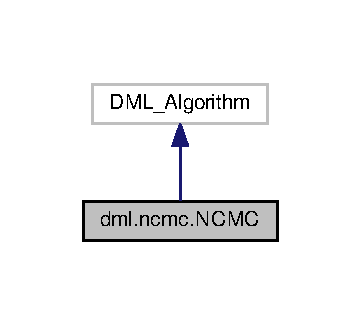
\includegraphics[width=173pt]{classdml_1_1ncmc_1_1NCMC__inherit__graph}
\end{center}
\end{figure}


Collaboration diagram for dml.\+ncmc.\+N\+C\+MC\+:
\nopagebreak
\begin{figure}[H]
\begin{center}
\leavevmode
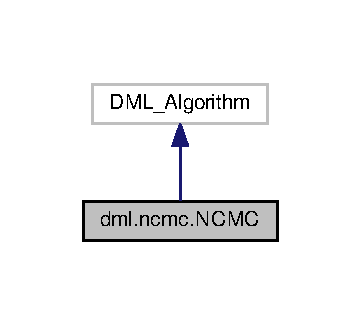
\includegraphics[width=173pt]{classdml_1_1ncmc_1_1NCMC__coll__graph}
\end{center}
\end{figure}
\subsection*{Public Member Functions}
\begin{DoxyCompactItemize}
\item 
def {\bfseries \+\_\+\+\_\+init\+\_\+\+\_\+} (self, num\+\_\+dims=None, centroids\+\_\+num=3, learning\+\_\+rate=\char`\"{}adaptive\char`\"{}, eta0=0.\+3, initial\+\_\+transform=None, max\+\_\+iter=300, tol=1e-\/15, prec=1e-\/15, descent\+\_\+method=\char`\"{}\+S\+G\+D\char`\"{}, eta\+\_\+thres=1e-\/14, learn\+\_\+inc=1.\+01, learn\+\_\+dec=0.\+5, kmeans\+\_\+kwargs)\hypertarget{classdml_1_1ncmc_1_1NCMC_a905f1d40b974485150080efa24733d5e}{}\label{classdml_1_1ncmc_1_1NCMC_a905f1d40b974485150080efa24733d5e}

\item 
def \hyperlink{classdml_1_1ncmc_1_1NCMC_a4d5a73df974b062e4f4d2f541e473a25}{metadata} (self)
\item 
def \hyperlink{classdml_1_1ncmc_1_1NCMC_a2744b247a6e0afba68ffe9ed51da5ad5}{transformer} (self)
\item 
def \hyperlink{classdml_1_1ncmc_1_1NCMC_a628e2c403fff6e06d8c7fcc24dd23440}{fit} (self, X, y)
\end{DoxyCompactItemize}
\subsection*{Public Attributes}
\begin{DoxyCompactItemize}
\item 
{\bfseries num\+\_\+dims\+\_\+}\hypertarget{classdml_1_1ncmc_1_1NCMC_a67faede3a06694e52a0a352085163baa}{}\label{classdml_1_1ncmc_1_1NCMC_a67faede3a06694e52a0a352085163baa}

\item 
{\bfseries L0\+\_\+}\hypertarget{classdml_1_1ncmc_1_1NCMC_a242497eba5bc9fe6323115a48b9248cc}{}\label{classdml_1_1ncmc_1_1NCMC_a242497eba5bc9fe6323115a48b9248cc}

\item 
{\bfseries max\+\_\+it\+\_\+}\hypertarget{classdml_1_1ncmc_1_1NCMC_a74c4ae0e92c8e695264b37f69b3d730a}{}\label{classdml_1_1ncmc_1_1NCMC_a74c4ae0e92c8e695264b37f69b3d730a}

\item 
{\bfseries eta\+\_\+}\hypertarget{classdml_1_1ncmc_1_1NCMC_aa1b6c1b93ca9f0aa01d6647fa76e08e8}{}\label{classdml_1_1ncmc_1_1NCMC_aa1b6c1b93ca9f0aa01d6647fa76e08e8}

\item 
{\bfseries eta0\+\_\+}\hypertarget{classdml_1_1ncmc_1_1NCMC_a1ab8a06bc261d1b77e591c204fd92fd7}{}\label{classdml_1_1ncmc_1_1NCMC_a1ab8a06bc261d1b77e591c204fd92fd7}

\item 
{\bfseries learning\+\_\+}\hypertarget{classdml_1_1ncmc_1_1NCMC_abddf783ace039f357afba48b7fdaaf2a}{}\label{classdml_1_1ncmc_1_1NCMC_abddf783ace039f357afba48b7fdaaf2a}

\item 
{\bfseries adaptive\+\_\+}\hypertarget{classdml_1_1ncmc_1_1NCMC_a5b8c46121373cb076fdd8b2a2dffa773}{}\label{classdml_1_1ncmc_1_1NCMC_a5b8c46121373cb076fdd8b2a2dffa773}

\item 
{\bfseries method\+\_\+}\hypertarget{classdml_1_1ncmc_1_1NCMC_a294c3834e2889d54994baf40b7662a94}{}\label{classdml_1_1ncmc_1_1NCMC_a294c3834e2889d54994baf40b7662a94}

\item 
{\bfseries eps\+\_\+}\hypertarget{classdml_1_1ncmc_1_1NCMC_acb4c399bc8771bddaa70c736809cc4d5}{}\label{classdml_1_1ncmc_1_1NCMC_acb4c399bc8771bddaa70c736809cc4d5}

\item 
{\bfseries tol\+\_\+}\hypertarget{classdml_1_1ncmc_1_1NCMC_a61d1495b8e2f4c064ebd7e0ef1e76686}{}\label{classdml_1_1ncmc_1_1NCMC_a61d1495b8e2f4c064ebd7e0ef1e76686}

\item 
{\bfseries etamin\+\_\+}\hypertarget{classdml_1_1ncmc_1_1NCMC_a40eb9f1a59eba0790c7090fe812717c4}{}\label{classdml_1_1ncmc_1_1NCMC_a40eb9f1a59eba0790c7090fe812717c4}

\item 
{\bfseries l\+\_\+inc\+\_\+}\hypertarget{classdml_1_1ncmc_1_1NCMC_ad9a6fb3682a18eac720f9325fec3c43a}{}\label{classdml_1_1ncmc_1_1NCMC_ad9a6fb3682a18eac720f9325fec3c43a}

\item 
{\bfseries l\+\_\+dec\+\_\+}\hypertarget{classdml_1_1ncmc_1_1NCMC_a04d0bf48715cd0627616248e4c27393d}{}\label{classdml_1_1ncmc_1_1NCMC_a04d0bf48715cd0627616248e4c27393d}

\item 
{\bfseries centroids\+\_\+num\+\_\+init\+\_\+}\hypertarget{classdml_1_1ncmc_1_1NCMC_ae313d6fa6deecbbb22dad07ba136d3f8}{}\label{classdml_1_1ncmc_1_1NCMC_ae313d6fa6deecbbb22dad07ba136d3f8}

\item 
{\bfseries kmeans\+\_\+kwargs\+\_\+}\hypertarget{classdml_1_1ncmc_1_1NCMC_a075d2a9fb68da758606b55a4b6a5bcc9}{}\label{classdml_1_1ncmc_1_1NCMC_a075d2a9fb68da758606b55a4b6a5bcc9}

\item 
{\bfseries num\+\_\+its\+\_\+}\hypertarget{classdml_1_1ncmc_1_1NCMC_a0bf55f870c9abde05ac30291df43b4f3}{}\label{classdml_1_1ncmc_1_1NCMC_a0bf55f870c9abde05ac30291df43b4f3}

\item 
{\bfseries initial\+\_\+expectance\+\_\+}\hypertarget{classdml_1_1ncmc_1_1NCMC_a990e271c53c0245ae6df6c8c1d7be8c6}{}\label{classdml_1_1ncmc_1_1NCMC_a990e271c53c0245ae6df6c8c1d7be8c6}

\item 
{\bfseries final\+\_\+expectance\+\_\+}\hypertarget{classdml_1_1ncmc_1_1NCMC_af3c9d6b2ea5d5f1bbe93257e130a7edb}{}\label{classdml_1_1ncmc_1_1NCMC_af3c9d6b2ea5d5f1bbe93257e130a7edb}

\item 
{\bfseries d\+\_\+}\hypertarget{classdml_1_1ncmc_1_1NCMC_af91ddd5d84ae4ae854d59af57f81131e}{}\label{classdml_1_1ncmc_1_1NCMC_af91ddd5d84ae4ae854d59af57f81131e}

\item 
{\bfseries nd\+\_\+}\hypertarget{classdml_1_1ncmc_1_1NCMC_ac2c635c38bd02a30dadb01ab750a86c6}{}\label{classdml_1_1ncmc_1_1NCMC_ac2c635c38bd02a30dadb01ab750a86c6}

\item 
{\bfseries L\+\_\+}\hypertarget{classdml_1_1ncmc_1_1NCMC_ac1113fea1d4cb668f4267ae17ef8090a}{}\label{classdml_1_1ncmc_1_1NCMC_ac1113fea1d4cb668f4267ae17ef8090a}

\item 
{\bfseries X\+\_\+}\hypertarget{classdml_1_1ncmc_1_1NCMC_abbaf2c9a61c10c46865fa00481902a54}{}\label{classdml_1_1ncmc_1_1NCMC_abbaf2c9a61c10c46865fa00481902a54}

\item 
{\bfseries y\+\_\+}\hypertarget{classdml_1_1ncmc_1_1NCMC_a08dc4ef78d2edb19c4ad1c35fcb85b6e}{}\label{classdml_1_1ncmc_1_1NCMC_a08dc4ef78d2edb19c4ad1c35fcb85b6e}

\item 
{\bfseries centroids\+\_\+num\+\_\+}\hypertarget{classdml_1_1ncmc_1_1NCMC_a0b6f1372cbc347c37924336f61c34aa7}{}\label{classdml_1_1ncmc_1_1NCMC_a0b6f1372cbc347c37924336f61c34aa7}

\item 
{\bfseries cs\+\_\+}\hypertarget{classdml_1_1ncmc_1_1NCMC_addc68abedb2aac2c113156054143a552}{}\label{classdml_1_1ncmc_1_1NCMC_addc68abedb2aac2c113156054143a552}

\end{DoxyCompactItemize}


\subsection{Detailed Description}
\begin{DoxyVerb}Nearest Class with Multiple Centroids distance metric learner (NCMC).

A distance metric learning algorithm to improve the nearest class with multiple centroids classifier.

Parameters
----------

num_dims : int, default=None

    Desired value for dimensionality reduction. If None, the dimension of transformed data will be the same as the original.

centroids_num : int, or list of int, default=3

    If it is a list, it must have the same size as the number of classes. In this case, i-th item will be the number of
    centroids to take in the i-th class. If it is an int, every class will have the same number of centroids.

learning_rate : string, default='adaptive'

    Type of learning rate update for gradient descent. Possible values are:

    - 'adaptive' : the learning rate will increase if the gradient step is succesful, else it will decrease.

    - 'constant' : the learning rate will be constant during all the gradient steps.

eta0 : int, default=0.3

    The initial value for learning rate.

initial_transform : 2D-Array or Matrix (d' x d), or string, default=None.

    If array or matrix that will represent the starting linear map for gradient descent, where d is the number of features,
    and d' is the dimension specified in num_dims.
    If None, euclidean distance will be used. If a string, the following values are allowed:

    - 'euclidean' : the euclidean distance.

    - 'scale' : a diagonal matrix that normalizes each attribute according to its range will be used.

max_iter : int, default=300

    Maximum number of gradient descent iterations.

prec : float, default=1e-15

    Precision stop criterion (gradient norm).

tol : float, default=1e-15

    Tolerance stop criterion (difference between two iterations)

descent_method : string, default='SGD'

    The descent method to use. Allowed values are:

    - 'SGD' : stochastic gradient descent.

    - 'BGD' : batch gradient descent.

eta_thres : float, default=1e-14

    A learning rate threshold stop criterion.

learn_inc : float, default=1.01

    Increase factor for learning rate. Ignored if learning_rate is not 'adaptive'.

learn_dec : float, default=0.5

    Decrease factor for learning rate. Ignored if learning_rate is not 'adaptive'.

References
----------
    Thomas Mensink et al. “Metric learning for large scale image classification: Generalizing to new
    classes at near-zero cost”. In: Computer Vision–ECCV 2012. Springer, 2012, pages 488-501.\end{DoxyVerb}
 

\subsection{Member Function Documentation}
\index{dml\+::ncmc\+::\+N\+C\+MC@{dml\+::ncmc\+::\+N\+C\+MC}!fit@{fit}}
\index{fit@{fit}!dml\+::ncmc\+::\+N\+C\+MC@{dml\+::ncmc\+::\+N\+C\+MC}}
\subsubsection[{\texorpdfstring{fit(self, X, y)}{fit(self, X, y)}}]{\setlength{\rightskip}{0pt plus 5cm}def dml.\+ncmc.\+N\+C\+M\+C.\+fit (
\begin{DoxyParamCaption}
\item[{}]{self, }
\item[{}]{X, }
\item[{}]{y}
\end{DoxyParamCaption}
)}\hypertarget{classdml_1_1ncmc_1_1NCMC_a628e2c403fff6e06d8c7fcc24dd23440}{}\label{classdml_1_1ncmc_1_1NCMC_a628e2c403fff6e06d8c7fcc24dd23440}
\begin{DoxyVerb}Fit the model from the data in X and the labels in y.

Parameters
----------
X : array-like, shape (N x d)
    Training vector, where N is the number of samples, and d is the number of features.

y : array-like, shape (N)
    Labels vector, where N is the number of samples.

Returns
-------
self : object
    Returns the instance itself.
\end{DoxyVerb}
 \index{dml\+::ncmc\+::\+N\+C\+MC@{dml\+::ncmc\+::\+N\+C\+MC}!metadata@{metadata}}
\index{metadata@{metadata}!dml\+::ncmc\+::\+N\+C\+MC@{dml\+::ncmc\+::\+N\+C\+MC}}
\subsubsection[{\texorpdfstring{metadata(self)}{metadata(self)}}]{\setlength{\rightskip}{0pt plus 5cm}def dml.\+ncmc.\+N\+C\+M\+C.\+metadata (
\begin{DoxyParamCaption}
\item[{}]{self}
\end{DoxyParamCaption}
)}\hypertarget{classdml_1_1ncmc_1_1NCMC_a4d5a73df974b062e4f4d2f541e473a25}{}\label{classdml_1_1ncmc_1_1NCMC_a4d5a73df974b062e4f4d2f541e473a25}
\begin{DoxyVerb}Obtains algorithm metadata.

Returns
-------
meta : A dictionary with the following metadata:
    - num_iters : Number of iterations that the descent method took.

    - initial_expectance : Initial value of the objective function (the expected score)

    - final_expectance : Final value of the objective function (the expected score)
\end{DoxyVerb}
 \index{dml\+::ncmc\+::\+N\+C\+MC@{dml\+::ncmc\+::\+N\+C\+MC}!transformer@{transformer}}
\index{transformer@{transformer}!dml\+::ncmc\+::\+N\+C\+MC@{dml\+::ncmc\+::\+N\+C\+MC}}
\subsubsection[{\texorpdfstring{transformer(self)}{transformer(self)}}]{\setlength{\rightskip}{0pt plus 5cm}def dml.\+ncmc.\+N\+C\+M\+C.\+transformer (
\begin{DoxyParamCaption}
\item[{}]{self}
\end{DoxyParamCaption}
)}\hypertarget{classdml_1_1ncmc_1_1NCMC_a2744b247a6e0afba68ffe9ed51da5ad5}{}\label{classdml_1_1ncmc_1_1NCMC_a2744b247a6e0afba68ffe9ed51da5ad5}
\begin{DoxyVerb}Obtains the learned projection.

Returns
-------
L : (d'xd) matrix, where d' is the desired output dimension and d is the number of features.
\end{DoxyVerb}
 

The documentation for this class was generated from the following file\+:\begin{DoxyCompactItemize}
\item 
dml/ncmc.\+pyx\end{DoxyCompactItemize}

\hypertarget{classdml_1_1ncmc_1_1NCMC__Classifier}{}\section{dml.\+ncmc.\+N\+C\+M\+C\+\_\+\+Classifier Class Reference}
\label{classdml_1_1ncmc_1_1NCMC__Classifier}\index{dml.\+ncmc.\+N\+C\+M\+C\+\_\+\+Classifier@{dml.\+ncmc.\+N\+C\+M\+C\+\_\+\+Classifier}}


Inheritance diagram for dml.\+ncmc.\+N\+C\+M\+C\+\_\+\+Classifier\+:
\nopagebreak
\begin{figure}[H]
\begin{center}
\leavevmode
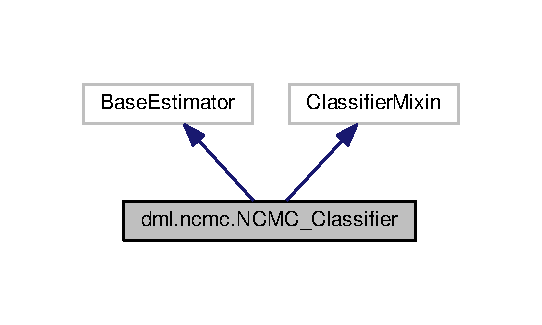
\includegraphics[width=260pt]{classdml_1_1ncmc_1_1NCMC__Classifier__inherit__graph}
\end{center}
\end{figure}


Collaboration diagram for dml.\+ncmc.\+N\+C\+M\+C\+\_\+\+Classifier\+:
\nopagebreak
\begin{figure}[H]
\begin{center}
\leavevmode
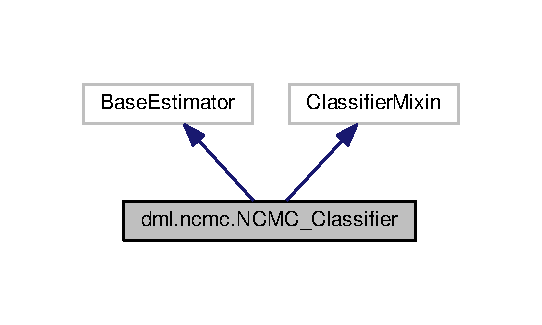
\includegraphics[width=260pt]{classdml_1_1ncmc_1_1NCMC__Classifier__coll__graph}
\end{center}
\end{figure}
\subsection*{Public Member Functions}
\begin{DoxyCompactItemize}
\item 
def {\bfseries \+\_\+\+\_\+init\+\_\+\+\_\+} (self, centroids\+\_\+num=3, kmeans\+\_\+kwargs)\hypertarget{classdml_1_1ncmc_1_1NCMC__Classifier_ab5bd6425900dacfc2899e6086653b64b}{}\label{classdml_1_1ncmc_1_1NCMC__Classifier_ab5bd6425900dacfc2899e6086653b64b}

\item 
def \hyperlink{classdml_1_1ncmc_1_1NCMC__Classifier_ad6afe7d5daca740d9d8542bafc6360c8}{fit} (self, X, y)
\item 
def \hyperlink{classdml_1_1ncmc_1_1NCMC__Classifier_af3a7507fd69eacaf0a53ce6fc0186e26}{predict} (self, X)
\end{DoxyCompactItemize}
\subsection*{Public Attributes}
\begin{DoxyCompactItemize}
\item 
{\bfseries centroids\+\_\+num\+\_\+}\hypertarget{classdml_1_1ncmc_1_1NCMC__Classifier_a210a5452a6e64215652a6ab0f35b1b67}{}\label{classdml_1_1ncmc_1_1NCMC__Classifier_a210a5452a6e64215652a6ab0f35b1b67}

\item 
{\bfseries kmeans\+\_\+args\+\_\+}\hypertarget{classdml_1_1ncmc_1_1NCMC__Classifier_a0f1cc3bf80a88c0120b69df89378c496}{}\label{classdml_1_1ncmc_1_1NCMC__Classifier_a0f1cc3bf80a88c0120b69df89378c496}

\item 
{\bfseries y\+\_\+}\hypertarget{classdml_1_1ncmc_1_1NCMC__Classifier_a917eb388dc06f4b844a09ef3b18bd6e6}{}\label{classdml_1_1ncmc_1_1NCMC__Classifier_a917eb388dc06f4b844a09ef3b18bd6e6}

\item 
{\bfseries le\+\_\+}\hypertarget{classdml_1_1ncmc_1_1NCMC__Classifier_a24b992cbeeb88a273ab0c929f3e4a453}{}\label{classdml_1_1ncmc_1_1NCMC__Classifier_a24b992cbeeb88a273ab0c929f3e4a453}

\item 
{\bfseries classes\+\_\+}\hypertarget{classdml_1_1ncmc_1_1NCMC__Classifier_a07590a630ae0bae7ceb795fee851c4e2}{}\label{classdml_1_1ncmc_1_1NCMC__Classifier_a07590a630ae0bae7ceb795fee851c4e2}

\item 
{\bfseries class\+\_\+map\+\_\+}\hypertarget{classdml_1_1ncmc_1_1NCMC__Classifier_ad6b75415bd91dbfe769f1f7027679520}{}\label{classdml_1_1ncmc_1_1NCMC__Classifier_ad6b75415bd91dbfe769f1f7027679520}

\item 
{\bfseries ncm\+\_\+}\hypertarget{classdml_1_1ncmc_1_1NCMC__Classifier_a87e5d19cc7240c865554f350cd10dc7c}{}\label{classdml_1_1ncmc_1_1NCMC__Classifier_a87e5d19cc7240c865554f350cd10dc7c}

\end{DoxyCompactItemize}


\subsection{Detailed Description}
\begin{DoxyVerb}Nearest Class with Multiple Centroids classifier.

A classifier that makes its predictions by choosing the class who has a centroid the nearest to the point.
For each class, an arbitrary number of centroids can be set. This centroids are calculated using k-Means
over each class sub-dataset.

Parameters
----------

centroids_num : int, or list of int, default=3

    If it is a list, it must have the same size as the number of classes. In this case, i-th item will be the number of
    centroids to take in the i-th class. If it is an int, every class will have the same number of centroids.

kmeans_args : dictionary

    Additional keyword args for k-Means.
\end{DoxyVerb}
 

\subsection{Member Function Documentation}
\index{dml\+::ncmc\+::\+N\+C\+M\+C\+\_\+\+Classifier@{dml\+::ncmc\+::\+N\+C\+M\+C\+\_\+\+Classifier}!fit@{fit}}
\index{fit@{fit}!dml\+::ncmc\+::\+N\+C\+M\+C\+\_\+\+Classifier@{dml\+::ncmc\+::\+N\+C\+M\+C\+\_\+\+Classifier}}
\subsubsection[{\texorpdfstring{fit(self, X, y)}{fit(self, X, y)}}]{\setlength{\rightskip}{0pt plus 5cm}def dml.\+ncmc.\+N\+C\+M\+C\+\_\+\+Classifier.\+fit (
\begin{DoxyParamCaption}
\item[{}]{self, }
\item[{}]{X, }
\item[{}]{y}
\end{DoxyParamCaption}
)}\hypertarget{classdml_1_1ncmc_1_1NCMC__Classifier_ad6afe7d5daca740d9d8542bafc6360c8}{}\label{classdml_1_1ncmc_1_1NCMC__Classifier_ad6afe7d5daca740d9d8542bafc6360c8}
\begin{DoxyVerb}Fit the model from the data in X and the labels in y.

Parameters
----------
X : array-like, shape (N x d)
    Training vector, where N is the number of samples, and d is the number of features.

y : array-like, shape (N)
    Labels vector, where N is the number of samples.

Returns
-------
self : object
    Returns the instance itself.
\end{DoxyVerb}
 \index{dml\+::ncmc\+::\+N\+C\+M\+C\+\_\+\+Classifier@{dml\+::ncmc\+::\+N\+C\+M\+C\+\_\+\+Classifier}!predict@{predict}}
\index{predict@{predict}!dml\+::ncmc\+::\+N\+C\+M\+C\+\_\+\+Classifier@{dml\+::ncmc\+::\+N\+C\+M\+C\+\_\+\+Classifier}}
\subsubsection[{\texorpdfstring{predict(self, X)}{predict(self, X)}}]{\setlength{\rightskip}{0pt plus 5cm}def dml.\+ncmc.\+N\+C\+M\+C\+\_\+\+Classifier.\+predict (
\begin{DoxyParamCaption}
\item[{}]{self, }
\item[{}]{X}
\end{DoxyParamCaption}
)}\hypertarget{classdml_1_1ncmc_1_1NCMC__Classifier_af3a7507fd69eacaf0a53ce6fc0186e26}{}\label{classdml_1_1ncmc_1_1NCMC__Classifier_af3a7507fd69eacaf0a53ce6fc0186e26}
\begin{DoxyVerb}Predicts the labels for the given data. Model needs to be already fitted.

X : 2D-Array or Matrix, default=None

    The dataset to be used. If None, the training set will be used. In this case, the prediction will be made
    using Leave One Out (that is, the sample to predict will be taken away from the training set).

Returns
-------

y : 1D-Array

    The vector with the label predictions.
\end{DoxyVerb}
 

The documentation for this class was generated from the following file\+:\begin{DoxyCompactItemize}
\item 
dml/ncmc.\+pyx\end{DoxyCompactItemize}

\hypertarget{classdml_1_1ncmml_1_1NCMML}{}\section{dml.\+ncmml.\+N\+C\+M\+ML Class Reference}
\label{classdml_1_1ncmml_1_1NCMML}\index{dml.\+ncmml.\+N\+C\+M\+ML@{dml.\+ncmml.\+N\+C\+M\+ML}}


Inheritance diagram for dml.\+ncmml.\+N\+C\+M\+ML\+:
\nopagebreak
\begin{figure}[H]
\begin{center}
\leavevmode
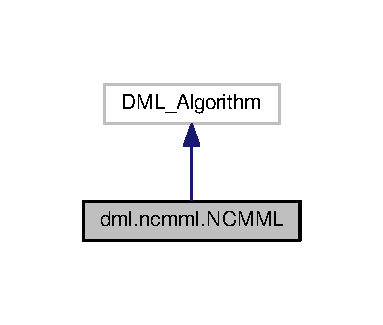
\includegraphics[width=184pt]{classdml_1_1ncmml_1_1NCMML__inherit__graph}
\end{center}
\end{figure}


Collaboration diagram for dml.\+ncmml.\+N\+C\+M\+ML\+:
\nopagebreak
\begin{figure}[H]
\begin{center}
\leavevmode
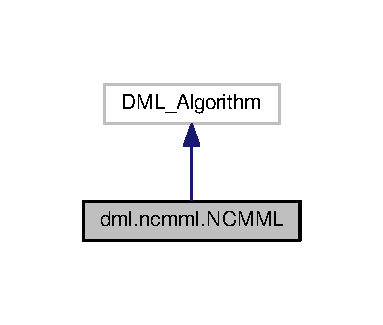
\includegraphics[width=184pt]{classdml_1_1ncmml_1_1NCMML__coll__graph}
\end{center}
\end{figure}
\subsection*{Public Member Functions}
\begin{DoxyCompactItemize}
\item 
def {\bfseries \+\_\+\+\_\+init\+\_\+\+\_\+} (self, num\+\_\+dims=None, learning\+\_\+rate=\char`\"{}adaptive\char`\"{}, eta0=0.\+3, initial\+\_\+transform=None, max\+\_\+iter=300, tol=1e-\/15, prec=1e-\/15, descent\+\_\+method=\char`\"{}\+S\+G\+D\char`\"{}, eta\+\_\+thres=1e-\/14, learn\+\_\+inc=1.\+01, learn\+\_\+dec=0.\+5)\hypertarget{classdml_1_1ncmml_1_1NCMML_ab8f65e9ec8d26077738d3773507c95af}{}\label{classdml_1_1ncmml_1_1NCMML_ab8f65e9ec8d26077738d3773507c95af}

\item 
def \hyperlink{classdml_1_1ncmml_1_1NCMML_a039f90483b5b4c964c937921f5c01abe}{metadata} (self)
\item 
def \hyperlink{classdml_1_1ncmml_1_1NCMML_aa2d6d578bc96c46689b8c185c3067df8}{transformer} (self)
\item 
def \hyperlink{classdml_1_1ncmml_1_1NCMML_a2c0c1cddd8eec63be977b3fb4866923a}{fit} (self, X, y)
\end{DoxyCompactItemize}
\subsection*{Public Attributes}
\begin{DoxyCompactItemize}
\item 
{\bfseries num\+\_\+dims\+\_\+}\hypertarget{classdml_1_1ncmml_1_1NCMML_a7a7b7e5b6f6e1c6137bc8c4f4966fe81}{}\label{classdml_1_1ncmml_1_1NCMML_a7a7b7e5b6f6e1c6137bc8c4f4966fe81}

\item 
{\bfseries L0\+\_\+}\hypertarget{classdml_1_1ncmml_1_1NCMML_aba8b2eb89d0d99dda734f2b423cbf786}{}\label{classdml_1_1ncmml_1_1NCMML_aba8b2eb89d0d99dda734f2b423cbf786}

\item 
{\bfseries max\+\_\+it\+\_\+}\hypertarget{classdml_1_1ncmml_1_1NCMML_aab51c46920445814d37b20d0e1d40b84}{}\label{classdml_1_1ncmml_1_1NCMML_aab51c46920445814d37b20d0e1d40b84}

\item 
{\bfseries eta\+\_\+}\hypertarget{classdml_1_1ncmml_1_1NCMML_a67709c04f6faf927b0f36fd3a8f47ae8}{}\label{classdml_1_1ncmml_1_1NCMML_a67709c04f6faf927b0f36fd3a8f47ae8}

\item 
{\bfseries eta0\+\_\+}\hypertarget{classdml_1_1ncmml_1_1NCMML_aa1a66e3579a51d8d65cda3e3a55eb5f7}{}\label{classdml_1_1ncmml_1_1NCMML_aa1a66e3579a51d8d65cda3e3a55eb5f7}

\item 
{\bfseries learning\+\_\+}\hypertarget{classdml_1_1ncmml_1_1NCMML_a56c65f669d9f92dbc686061a7cf49d27}{}\label{classdml_1_1ncmml_1_1NCMML_a56c65f669d9f92dbc686061a7cf49d27}

\item 
{\bfseries adaptive\+\_\+}\hypertarget{classdml_1_1ncmml_1_1NCMML_a5338e43bd3edd2fb27bafe465843b4cb}{}\label{classdml_1_1ncmml_1_1NCMML_a5338e43bd3edd2fb27bafe465843b4cb}

\item 
{\bfseries method\+\_\+}\hypertarget{classdml_1_1ncmml_1_1NCMML_a53ade464e911bfd448bdcc831f8b9b62}{}\label{classdml_1_1ncmml_1_1NCMML_a53ade464e911bfd448bdcc831f8b9b62}

\item 
{\bfseries eps\+\_\+}\hypertarget{classdml_1_1ncmml_1_1NCMML_ad78723654662dc2cddff99f27439400b}{}\label{classdml_1_1ncmml_1_1NCMML_ad78723654662dc2cddff99f27439400b}

\item 
{\bfseries tol\+\_\+}\hypertarget{classdml_1_1ncmml_1_1NCMML_ad205f159e63da5a4e27e7193df0d97c0}{}\label{classdml_1_1ncmml_1_1NCMML_ad205f159e63da5a4e27e7193df0d97c0}

\item 
{\bfseries etamin\+\_\+}\hypertarget{classdml_1_1ncmml_1_1NCMML_a5b540c37775e7f957259a997e280b376}{}\label{classdml_1_1ncmml_1_1NCMML_a5b540c37775e7f957259a997e280b376}

\item 
{\bfseries l\+\_\+inc\+\_\+}\hypertarget{classdml_1_1ncmml_1_1NCMML_ad8f2d336393c35f8e6a60817372e54fa}{}\label{classdml_1_1ncmml_1_1NCMML_ad8f2d336393c35f8e6a60817372e54fa}

\item 
{\bfseries l\+\_\+dec\+\_\+}\hypertarget{classdml_1_1ncmml_1_1NCMML_a091cdec44d78c87cb3a82d226b2e9146}{}\label{classdml_1_1ncmml_1_1NCMML_a091cdec44d78c87cb3a82d226b2e9146}

\item 
{\bfseries num\+\_\+its\+\_\+}\hypertarget{classdml_1_1ncmml_1_1NCMML_abfc452a41f73f17183331a4713c22302}{}\label{classdml_1_1ncmml_1_1NCMML_abfc452a41f73f17183331a4713c22302}

\item 
{\bfseries initial\+\_\+expectance\+\_\+}\hypertarget{classdml_1_1ncmml_1_1NCMML_ae424f09f9828d9c8e4fac9211b1a1586}{}\label{classdml_1_1ncmml_1_1NCMML_ae424f09f9828d9c8e4fac9211b1a1586}

\item 
{\bfseries final\+\_\+expectance\+\_\+}\hypertarget{classdml_1_1ncmml_1_1NCMML_ade93bd8d6bf766205d85b1e9bbb33079}{}\label{classdml_1_1ncmml_1_1NCMML_ade93bd8d6bf766205d85b1e9bbb33079}

\item 
{\bfseries d\+\_\+}\hypertarget{classdml_1_1ncmml_1_1NCMML_a12a3da3b328a1e3c19ac3f94b5198b31}{}\label{classdml_1_1ncmml_1_1NCMML_a12a3da3b328a1e3c19ac3f94b5198b31}

\item 
{\bfseries nd\+\_\+}\hypertarget{classdml_1_1ncmml_1_1NCMML_a5fe286a4ad41e61e6d2170646173e7c5}{}\label{classdml_1_1ncmml_1_1NCMML_a5fe286a4ad41e61e6d2170646173e7c5}

\item 
{\bfseries L\+\_\+}\hypertarget{classdml_1_1ncmml_1_1NCMML_aaf28d14f62f533bf1aefe2221c3e9a80}{}\label{classdml_1_1ncmml_1_1NCMML_aaf28d14f62f533bf1aefe2221c3e9a80}

\item 
{\bfseries X\+\_\+}\hypertarget{classdml_1_1ncmml_1_1NCMML_ad14e5ca754753b16242b6a1a3b0816a2}{}\label{classdml_1_1ncmml_1_1NCMML_ad14e5ca754753b16242b6a1a3b0816a2}

\item 
{\bfseries y\+\_\+}\hypertarget{classdml_1_1ncmml_1_1NCMML_a31fb1f0fd8032ec6c9b37ddd31aa1098}{}\label{classdml_1_1ncmml_1_1NCMML_a31fb1f0fd8032ec6c9b37ddd31aa1098}

\item 
{\bfseries centroids\+\_\+}\hypertarget{classdml_1_1ncmml_1_1NCMML_a54514205517c532362e6d40a5ba26e51}{}\label{classdml_1_1ncmml_1_1NCMML_a54514205517c532362e6d40a5ba26e51}

\end{DoxyCompactItemize}


\subsection{Detailed Description}
\begin{DoxyVerb}Nearest Class Mean Metric Learning (NCMML)

A distance metric learning algorithm to improve the nearest class mean classifier.

Parameters
----------

num_dims : int, default=None

    Desired value for dimensionality reduction. If None, the dimension of transformed data will be the same as the original.

learning_rate : string, default='adaptive'

    Type of learning rate update for gradient descent. Possible values are:

    - 'adaptive' : the learning rate will increase if the gradient step is succesful, else it will decrease.

    - 'constant' : the learning rate will be constant during all the gradient steps.

eta0 : int, default=0.3

    The initial value for learning rate.

initial_transform : 2D-Array or Matrix (d' x d), or string, default=None.

    If array or matrix that will represent the starting linear map for gradient descent, where d is the number of features,
    and d' is the dimension specified in num_dims.
    If None, euclidean distance will be used. If a string, the following values are allowed:

    - 'euclidean' : the euclidean distance.

    - 'scale' : a diagonal matrix that normalizes each attribute according to its range will be used.

max_iter : int, default=300

    Maximum number of gradient descent iterations.

prec : float, default=1e-15

    Precision stop criterion (gradient norm).

tol : float, default=1e-15

    Tolerance stop criterion (difference between two iterations)

descent_method : string, default='SGD'

    The descent method to use. Allowed values are:

    - 'SGD' : stochastic gradient descent.

    - 'BGD' : batch gradient descent.

eta_thres : float, default=1e-14

    A learning rate threshold stop criterion.

learn_inc : float, default=1.01

    Increase factor for learning rate. Ignored if learning_rate is not 'adaptive'.

learn_dec : float, default=0.5

    Decrease factor for learning rate. Ignored if learning_rate is not 'adaptive'.

References
----------
    Thomas Mensink et al. “Metric learning for large scale image classification: Generalizing to new
    classes at near-zero cost”. In: Computer Vision–ECCV 2012. Springer, 2012, pages 488-501.\end{DoxyVerb}
 

\subsection{Member Function Documentation}
\index{dml\+::ncmml\+::\+N\+C\+M\+ML@{dml\+::ncmml\+::\+N\+C\+M\+ML}!fit@{fit}}
\index{fit@{fit}!dml\+::ncmml\+::\+N\+C\+M\+ML@{dml\+::ncmml\+::\+N\+C\+M\+ML}}
\subsubsection[{\texorpdfstring{fit(self, X, y)}{fit(self, X, y)}}]{\setlength{\rightskip}{0pt plus 5cm}def dml.\+ncmml.\+N\+C\+M\+M\+L.\+fit (
\begin{DoxyParamCaption}
\item[{}]{self, }
\item[{}]{X, }
\item[{}]{y}
\end{DoxyParamCaption}
)}\hypertarget{classdml_1_1ncmml_1_1NCMML_a2c0c1cddd8eec63be977b3fb4866923a}{}\label{classdml_1_1ncmml_1_1NCMML_a2c0c1cddd8eec63be977b3fb4866923a}
\begin{DoxyVerb}Fit the model from the data in X and the labels in y.

Parameters
----------
X : array-like, shape (N x d)
    Training vector, where N is the number of samples, and d is the number of features.

y : array-like, shape (N)
    Labels vector, where N is the number of samples.

Returns
-------
self : object
    Returns the instance itself.
\end{DoxyVerb}
 \index{dml\+::ncmml\+::\+N\+C\+M\+ML@{dml\+::ncmml\+::\+N\+C\+M\+ML}!metadata@{metadata}}
\index{metadata@{metadata}!dml\+::ncmml\+::\+N\+C\+M\+ML@{dml\+::ncmml\+::\+N\+C\+M\+ML}}
\subsubsection[{\texorpdfstring{metadata(self)}{metadata(self)}}]{\setlength{\rightskip}{0pt plus 5cm}def dml.\+ncmml.\+N\+C\+M\+M\+L.\+metadata (
\begin{DoxyParamCaption}
\item[{}]{self}
\end{DoxyParamCaption}
)}\hypertarget{classdml_1_1ncmml_1_1NCMML_a039f90483b5b4c964c937921f5c01abe}{}\label{classdml_1_1ncmml_1_1NCMML_a039f90483b5b4c964c937921f5c01abe}
\begin{DoxyVerb}Obtains algorithm metadata.

Returns
-------
meta : A dictionary with the following metadata:
    - num_iters : Number of iterations that the descent method took.

    - initial_expectance : Initial value of the objective function (the expected score)

    - final_expectance : Final value of the objective function (the expected score)
\end{DoxyVerb}
 \index{dml\+::ncmml\+::\+N\+C\+M\+ML@{dml\+::ncmml\+::\+N\+C\+M\+ML}!transformer@{transformer}}
\index{transformer@{transformer}!dml\+::ncmml\+::\+N\+C\+M\+ML@{dml\+::ncmml\+::\+N\+C\+M\+ML}}
\subsubsection[{\texorpdfstring{transformer(self)}{transformer(self)}}]{\setlength{\rightskip}{0pt plus 5cm}def dml.\+ncmml.\+N\+C\+M\+M\+L.\+transformer (
\begin{DoxyParamCaption}
\item[{}]{self}
\end{DoxyParamCaption}
)}\hypertarget{classdml_1_1ncmml_1_1NCMML_aa2d6d578bc96c46689b8c185c3067df8}{}\label{classdml_1_1ncmml_1_1NCMML_aa2d6d578bc96c46689b8c185c3067df8}
\begin{DoxyVerb}Obtains algorithm metadata.

Returns
-------
meta : A dictionary with the following metadata:
    - num_iters : Number of iterations that the descent method took.

    - initial_expectance : Initial value of the objective function (the expected score)

    - final_expectance : Final value of the objective function (the expected score)
\end{DoxyVerb}
 

The documentation for this class was generated from the following file\+:\begin{DoxyCompactItemize}
\item 
dml/ncmml.\+pyx\end{DoxyCompactItemize}

\hypertarget{classdml_1_1pca_1_1PCA}{}\section{dml.\+pca.\+P\+CA Class Reference}
\label{classdml_1_1pca_1_1PCA}\index{dml.\+pca.\+P\+CA@{dml.\+pca.\+P\+CA}}


Inheritance diagram for dml.\+pca.\+P\+CA\+:
\nopagebreak
\begin{figure}[H]
\begin{center}
\leavevmode
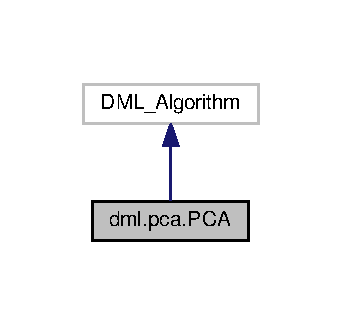
\includegraphics[width=164pt]{classdml_1_1pca_1_1PCA__inherit__graph}
\end{center}
\end{figure}


Collaboration diagram for dml.\+pca.\+P\+CA\+:
\nopagebreak
\begin{figure}[H]
\begin{center}
\leavevmode
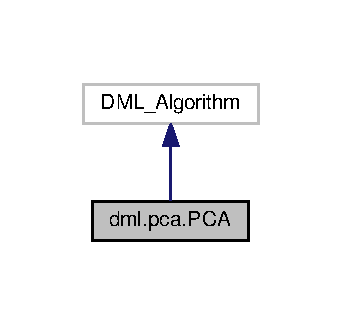
\includegraphics[width=164pt]{classdml_1_1pca_1_1PCA__coll__graph}
\end{center}
\end{figure}
\subsection*{Public Member Functions}
\begin{DoxyCompactItemize}
\item 
def {\bfseries \+\_\+\+\_\+init\+\_\+\+\_\+} (self, num\+\_\+dims=None, thres=None)\hypertarget{classdml_1_1pca_1_1PCA_a55d22d08e5f8617a880ac3af1dc355e2}{}\label{classdml_1_1pca_1_1PCA_a55d22d08e5f8617a880ac3af1dc355e2}

\item 
def \hyperlink{classdml_1_1pca_1_1PCA_a1a7f105ce4a9de19117b92c441ff53f5}{transformer} (self)
\item 
def \hyperlink{classdml_1_1pca_1_1PCA_a1e4361b3ecc20bbc7b1037739abb2101}{metadata} (self)
\item 
def \hyperlink{classdml_1_1pca_1_1PCA_a477310831a7b669598fb8d46b0700bb1}{fit} (self, X, y=None)
\item 
def \hyperlink{classdml_1_1pca_1_1PCA_a8c0378940c6a8c80952ffe2f1d582b54}{transform} (self, X=None)
\end{DoxyCompactItemize}
\subsection*{Public Attributes}
\begin{DoxyCompactItemize}
\item 
{\bfseries num\+\_\+dims\+\_\+}\hypertarget{classdml_1_1pca_1_1PCA_a322b92ba0a03ff203bcddce294ed7408}{}\label{classdml_1_1pca_1_1PCA_a322b92ba0a03ff203bcddce294ed7408}

\item 
{\bfseries thres\+\_\+}\hypertarget{classdml_1_1pca_1_1PCA_a50accdad08436d9aa31f3d7ffbb8b299}{}\label{classdml_1_1pca_1_1PCA_a50accdad08436d9aa31f3d7ffbb8b299}

\item 
{\bfseries skpca\+\_\+}\hypertarget{classdml_1_1pca_1_1PCA_a45d491dea24b8523052a37ba67940956}{}\label{classdml_1_1pca_1_1PCA_a45d491dea24b8523052a37ba67940956}

\item 
{\bfseries nd\+\_\+}\hypertarget{classdml_1_1pca_1_1PCA_af3f7399bf5dfd2a8c8184977948ebd6b}{}\label{classdml_1_1pca_1_1PCA_af3f7399bf5dfd2a8c8184977948ebd6b}

\item 
{\bfseries acum\+\_\+eig\+\_\+}\hypertarget{classdml_1_1pca_1_1PCA_ad55373256e1a1aaa2d5bd15584f4e66f}{}\label{classdml_1_1pca_1_1PCA_ad55373256e1a1aaa2d5bd15584f4e66f}

\item 
{\bfseries X\+\_\+}\hypertarget{classdml_1_1pca_1_1PCA_a974558b32be9516cec8b521bb510c954}{}\label{classdml_1_1pca_1_1PCA_a974558b32be9516cec8b521bb510c954}

\item 
{\bfseries d\+\_\+}\hypertarget{classdml_1_1pca_1_1PCA_a766dedaab2915d2280102e27b056ef2c}{}\label{classdml_1_1pca_1_1PCA_a766dedaab2915d2280102e27b056ef2c}

\item 
{\bfseries explained\+\_\+variance\+\_\+}\hypertarget{classdml_1_1pca_1_1PCA_a533c1573899bd56321015e53ad95de3e}{}\label{classdml_1_1pca_1_1PCA_a533c1573899bd56321015e53ad95de3e}

\item 
{\bfseries acum\+\_\+variance\+\_\+}\hypertarget{classdml_1_1pca_1_1PCA_ac2992174c11c86a9261d43b3e0a0c0aa}{}\label{classdml_1_1pca_1_1PCA_ac2992174c11c86a9261d43b3e0a0c0aa}

\item 
{\bfseries L\+\_\+}\hypertarget{classdml_1_1pca_1_1PCA_a7d9c1db0aa3d6c7bff9e6d181a53d211}{}\label{classdml_1_1pca_1_1PCA_a7d9c1db0aa3d6c7bff9e6d181a53d211}

\end{DoxyCompactItemize}


\subsection{Detailed Description}
\begin{DoxyVerb}Principal Component Analysis (PCA)

A distance metric learning algorithm for unsupervised dimensionality reduction, obtaining orthogonal directions that maximize the variance.
This class is a wrapper for :class:`~sklearn.decomposition.PCA`.

Parameters
----------

num_dims : int, default=None

    Number of components for dimensionality reduction. If None, all the principal components will be taken. Ignored if thres is provided.

thres : float

    Fraction of variability to keep, from 0 to 1. Data dimension will be reduced until the lowest dimension that keeps 'thres' explained variance.
\end{DoxyVerb}
 

\subsection{Member Function Documentation}
\index{dml\+::pca\+::\+P\+CA@{dml\+::pca\+::\+P\+CA}!fit@{fit}}
\index{fit@{fit}!dml\+::pca\+::\+P\+CA@{dml\+::pca\+::\+P\+CA}}
\subsubsection[{\texorpdfstring{fit(self, X, y=\+None)}{fit(self, X, y=None)}}]{\setlength{\rightskip}{0pt plus 5cm}def dml.\+pca.\+P\+C\+A.\+fit (
\begin{DoxyParamCaption}
\item[{}]{self, }
\item[{}]{X, }
\item[{}]{y = {\ttfamily None}}
\end{DoxyParamCaption}
)}\hypertarget{classdml_1_1pca_1_1PCA_a477310831a7b669598fb8d46b0700bb1}{}\label{classdml_1_1pca_1_1PCA_a477310831a7b669598fb8d46b0700bb1}
\begin{DoxyVerb}Fit the model from the data in X and the labels in y.

Parameters
----------
X : array-like, shape (N x d)
    Training vector, where N is the number of samples, and d is the number of features.

y : array-like, shape (N)
    Labels vector, where N is the number of samples.

Returns
-------
self : object
    Returns the instance itself.
\end{DoxyVerb}
 \index{dml\+::pca\+::\+P\+CA@{dml\+::pca\+::\+P\+CA}!metadata@{metadata}}
\index{metadata@{metadata}!dml\+::pca\+::\+P\+CA@{dml\+::pca\+::\+P\+CA}}
\subsubsection[{\texorpdfstring{metadata(self)}{metadata(self)}}]{\setlength{\rightskip}{0pt plus 5cm}def dml.\+pca.\+P\+C\+A.\+metadata (
\begin{DoxyParamCaption}
\item[{}]{self}
\end{DoxyParamCaption}
)}\hypertarget{classdml_1_1pca_1_1PCA_a1e4361b3ecc20bbc7b1037739abb2101}{}\label{classdml_1_1pca_1_1PCA_a1e4361b3ecc20bbc7b1037739abb2101}
\begin{DoxyVerb}Obtains algorithm metadata.

Returns
-------
meta : A dictionary with the following metadata:
    num_dims : dimension of the reduced data.

    acum_eig : eigenvalue rate accumulated in the learned output respect to the total dimension.
\end{DoxyVerb}
 \index{dml\+::pca\+::\+P\+CA@{dml\+::pca\+::\+P\+CA}!transform@{transform}}
\index{transform@{transform}!dml\+::pca\+::\+P\+CA@{dml\+::pca\+::\+P\+CA}}
\subsubsection[{\texorpdfstring{transform(self, X=\+None)}{transform(self, X=None)}}]{\setlength{\rightskip}{0pt plus 5cm}def dml.\+pca.\+P\+C\+A.\+transform (
\begin{DoxyParamCaption}
\item[{}]{self, }
\item[{}]{X = {\ttfamily None}}
\end{DoxyParamCaption}
)}\hypertarget{classdml_1_1pca_1_1PCA_a8c0378940c6a8c80952ffe2f1d582b54}{}\label{classdml_1_1pca_1_1PCA_a8c0378940c6a8c80952ffe2f1d582b54}
\begin{DoxyVerb}Applies the kernel transformation.

Parameters
----------
X : (N x d) matrix, optional
    Data to transform. If not supplied, the training data will be used.

Returns
-------
transformed: (N x d') matrix.
    Input data transformed by the learned mapping.
\end{DoxyVerb}
 \index{dml\+::pca\+::\+P\+CA@{dml\+::pca\+::\+P\+CA}!transformer@{transformer}}
\index{transformer@{transformer}!dml\+::pca\+::\+P\+CA@{dml\+::pca\+::\+P\+CA}}
\subsubsection[{\texorpdfstring{transformer(self)}{transformer(self)}}]{\setlength{\rightskip}{0pt plus 5cm}def dml.\+pca.\+P\+C\+A.\+transformer (
\begin{DoxyParamCaption}
\item[{}]{self}
\end{DoxyParamCaption}
)}\hypertarget{classdml_1_1pca_1_1PCA_a1a7f105ce4a9de19117b92c441ff53f5}{}\label{classdml_1_1pca_1_1PCA_a1a7f105ce4a9de19117b92c441ff53f5}
\begin{DoxyVerb}Obtains the learned projection.

Returns
-------
L : (d'xd) matrix, where d' is the desired output dimension and d is the number of features.
\end{DoxyVerb}
 

The documentation for this class was generated from the following file\+:\begin{DoxyCompactItemize}
\item 
dml/pca.\+pyx\end{DoxyCompactItemize}

\hypertarget{classdml_1_1base_1_1Transformer}{}\section{dml.\+base.\+Transformer Class Reference}
\label{classdml_1_1base_1_1Transformer}\index{dml.\+base.\+Transformer@{dml.\+base.\+Transformer}}


Inheritance diagram for dml.\+base.\+Transformer\+:\nopagebreak
\begin{figure}[H]
\begin{center}
\leavevmode
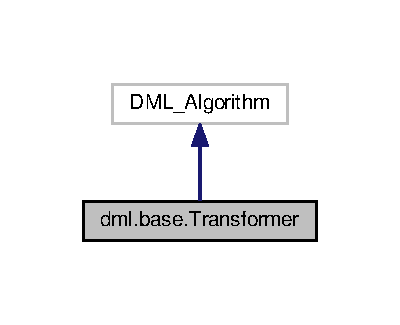
\includegraphics[width=192pt]{classdml_1_1base_1_1Transformer__inherit__graph}
\end{center}
\end{figure}


Collaboration diagram for dml.\+base.\+Transformer\+:\nopagebreak
\begin{figure}[H]
\begin{center}
\leavevmode
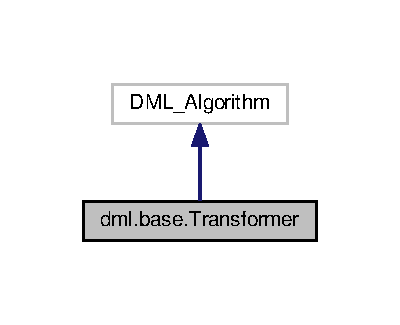
\includegraphics[width=192pt]{classdml_1_1base_1_1Transformer__coll__graph}
\end{center}
\end{figure}
\subsection*{Public Member Functions}
\begin{DoxyCompactItemize}
\item 
def {\bfseries \+\_\+\+\_\+init\+\_\+\+\_\+} (self, \hyperlink{classdml_1_1base_1_1Transformer_a141897f784dd19a70fa72f4154751881}{transformer})\hypertarget{classdml_1_1base_1_1Transformer_ac4abe61c0b5af45b0a11de4f872a6fc3}{}\label{classdml_1_1base_1_1Transformer_ac4abe61c0b5af45b0a11de4f872a6fc3}

\item 
def \hyperlink{classdml_1_1base_1_1Transformer_a13ce455fe423e55f0ffa41c47a080c55}{fit} (self, X, y)
\item 
def \hyperlink{classdml_1_1base_1_1Transformer_a141897f784dd19a70fa72f4154751881}{transformer} (self)
\end{DoxyCompactItemize}
\subsection*{Public Attributes}
\begin{DoxyCompactItemize}
\item 
{\bfseries L\+\_\+}\hypertarget{classdml_1_1base_1_1Transformer_ae545c8d86053bddf2ed9c34308462406}{}\label{classdml_1_1base_1_1Transformer_ae545c8d86053bddf2ed9c34308462406}

\item 
{\bfseries y\+\_\+}\hypertarget{classdml_1_1base_1_1Transformer_ab3cf89b17477747577644c6ebf292569}{}\label{classdml_1_1base_1_1Transformer_ab3cf89b17477747577644c6ebf292569}

\end{DoxyCompactItemize}


\subsection{Detailed Description}
\begin{DoxyVerb}A DML algorithm that defines a distance given a linear transformation.

Parameters
----------

transformer : (d' x d) matrix, representing a linear transformacion from d-dimensional euclidean space
              to d'-dimensional euclidean space.
\end{DoxyVerb}
 

\subsection{Member Function Documentation}
\index{dml\+::base\+::\+Transformer@{dml\+::base\+::\+Transformer}!fit@{fit}}
\index{fit@{fit}!dml\+::base\+::\+Transformer@{dml\+::base\+::\+Transformer}}
\subsubsection[{\texorpdfstring{fit(self, X, y)}{fit(self, X, y)}}]{\setlength{\rightskip}{0pt plus 5cm}def dml.\+base.\+Transformer.\+fit (
\begin{DoxyParamCaption}
\item[{}]{self, }
\item[{}]{X, }
\item[{}]{y}
\end{DoxyParamCaption}
)}\hypertarget{classdml_1_1base_1_1Transformer_a13ce455fe423e55f0ffa41c47a080c55}{}\label{classdml_1_1base_1_1Transformer_a13ce455fe423e55f0ffa41c47a080c55}
\begin{DoxyVerb}Fit the model from the data in X and the labels in y.

Parameters
----------
X : array-like, shape (N x d)
    Training vector, where N is the number of samples, and d is the number of features.

y : array-like, shape (N)
    Labels vector, where N is the number of samples.

Returns
-------
self : object
    Returns the instance itself.
\end{DoxyVerb}
 \index{dml\+::base\+::\+Transformer@{dml\+::base\+::\+Transformer}!transformer@{transformer}}
\index{transformer@{transformer}!dml\+::base\+::\+Transformer@{dml\+::base\+::\+Transformer}}
\subsubsection[{\texorpdfstring{transformer(self)}{transformer(self)}}]{\setlength{\rightskip}{0pt plus 5cm}def dml.\+base.\+Transformer.\+transformer (
\begin{DoxyParamCaption}
\item[{}]{self}
\end{DoxyParamCaption}
)}\hypertarget{classdml_1_1base_1_1Transformer_a141897f784dd19a70fa72f4154751881}{}\label{classdml_1_1base_1_1Transformer_a141897f784dd19a70fa72f4154751881}
\begin{DoxyVerb}Obtains the learned projection.

Returns
-------
L : (d'xd) matrix, where d' is the desired output dimension and d is the number of features.
\end{DoxyVerb}
 

The documentation for this class was generated from the following file\+:\begin{DoxyCompactItemize}
\item 
dml/base.\+py\end{DoxyCompactItemize}

%--- End generated contents ---

% Index
\backmatter
\newpage
\phantomsection
\clearemptydoublepage
\addcontentsline{toc}{chapter}{Index}
\printindex

\end{document}
